\documentclass[a4paper]{book}
\usepackage[utf8]{inputenc}
\usepackage{graphicx}
\usepackage[fontsize=12.0pt]{fontsize}
\usepackage{amsmath}
\usepackage[english]{babel}
\usepackage{mathrsfs}

% For subplot - does not work...
% \usepackage{graphicx}
% \usepackage{subcaption}
% \usepackage{mwe}

% For blue click-to-go reference
\usepackage[table]{xcolor}
\definecolor{ashgrey}{rgb}{0.7, 0.75, 0.71}
\definecolor{ao(english)}{rgb}{0.0, 0.5, 0.0}

\usepackage{hyperref}
	\hypersetup{
		colorlinks=true,
		linkcolor=blue,
		filecolor=magenta,      
		urlcolor=cyan,
		citecolor=ao(english)
	}
\hypersetup{linktocpage}
\usepackage{floatrow}
% Table float box with bottom caption, box width adjusted to content
\usepackage{multirow}
\newfloatcommand{capbtabbox}{table}[][\FBwidth]

% Keywords command
\providecommand{\keywords}[1]
{
  \small	
  \textbf{\textit{Keywords:}} #1
}

\usepackage[a4paper, total={6in, 9in}]{geometry}
\usepackage{url}
\usepackage{fancyhdr}
\usepackage[toc,page]{appendix}
\usepackage{amsthm}
\newtheorem{theorem}{Theorem}
\usepackage{amssymb}
\usepackage{amsmath}
\usepackage{hyperref}
\usepackage{xifthen}
\usepackage{xparse}
\usepackage{dsfont}


% To write pseudo code
\usepackage[ruled,vlined]{algorithm2e}
\SetKwInput{KwInput}{Input}
\SetKwInput{KwOutput}{Output}
\SetKwInput{Function}{function}




\usepackage{neuralnetwork}
\usepackage{lastpage}
\usepackage{natbib}
% -------------- Nomenclature settings ------------
\usepackage[intoc]{nomencl}
\makenomenclature
\renewcommand{\nomname}{Notation}
\renewcommand{\nompreamble}{This section provides a concise reference describing the notation used throughout
this dissertation.}
\usepackage{etoolbox}
\renewcommand\nomgroup[1]{%
  \item[\bfseries
  \ifstrequal{#1}{N}{Numbers and Arrays}{%
  \ifstrequal{#1}{S}{Sets and Graphs}{%
  \ifstrequal{#1}{I}{Indexing}{%
  \ifstrequal{#1}{L}{Linear Algebra Operations}{%
  \ifstrequal{#1}{P}{Probability and Information Theory}{%
  \ifstrequal{#1}{D}{Datasets and Distributions}{
  \ifstrequal{#1}{F}{Functions}{}
  }}}}}
  }%
]}
% --------------------------------------------------


% ------- For python-code format and highligting ---
% Default fixed font does not support bold face
\DeclareFixedFont{\ttb}{T1}{txtt}{bx}{n}{12} % for bold
\DeclareFixedFont{\ttm}{T1}{txtt}{m}{n}{12}  % for normal

% code listings for python
\usepackage{listings}

\lstdefinestyle{mystyle}{
	language=Python,
	basicstyle=\ttfamily\footnotesize,
	backgroundcolor=\color[HTML]{F7F7F7},
	rulecolor=\color[HTML]{EEEEEE},
	identifierstyle=\color[HTML]{24292E},
	emphstyle=\color[HTML]{005CC5},
	keywordstyle=\color[HTML]{D73A49},
	commentstyle=\color[HTML]{6A737D},
	stringstyle=\color[HTML]{032F62},
	emph={@property,self,range,True,False},
	morekeywords={super,with,as,lambda},
	literate=%
	{+}{{{\color[HTML]{D73A49}+}}}1
	{-}{{{\color[HTML]{D73A49}-}}}1
	{*}{{{\color[HTML]{D73A49}*}}}1
	{/}{{{\color[HTML]{D73A49}/}}}1
	{=}{{{\color[HTML]{D73A49}=}}}1
	{/=}{{{\color[HTML]{D73A49}=}}}1,
	breakatwhitespace=false,
	breaklines=true,
	captionpos=b,
	keepspaces=true,
	numbers=none,
	showspaces=false,
	showstringspaces=false,
	showtabs=false,
	tabsize=4,
	frame=single,
}
\lstset{style=mystyle}

%---------------------------- Macros  -----------------
% Left-right bracket
\newcommand{\lr}[1]{\left (#1\right)}
% Left-right square bracket
\newcommand{\lrs}[1]{\left [#1 \right]}
% Left-right curly bracket
\newcommand{\lrc}[1]{\left \{#1\right\}}
% Left-right absolute value
\newcommand{\lra}[1]{\left |#1\right|}
% Left-right upper value
\newcommand{\lru}[1]{\left \lceil#1\right\rceil}
% Scalar product
\newcommand{\vp}[2]{\left \langle #1 , #2 \right \rangle}
% The real numbers
\newcommand{\R}{\mathbb R}
% The natural numbers
\newcommand{\N}{\mathbb N}
% Expectation symbol with an optional argument
\NewDocumentCommand{\E}{o}{\mathbb E\IfValueT{#1}{\lrs{#1}}}
% Indicator function with an optional argument
\NewDocumentCommand{\1}{o}{\mathds 1{\IfValueT{#1}{\lr{#1}}}}
% Probability function
\let\P\undefined
\NewDocumentCommand{\P}{o}{\mathbb P{\IfValueT{#1}{\lr{#1}}}}
% A hypothesis space
\newcommand{\HH}{\mathcal H}
% A sample space
\newcommand{\XX}{\mathbb{X}}
% A label space
\newcommand{\YY}{\mathbb{Y}}
% A nicer emptyset symbol
\let\emptyset\varnothing
% Sign operator
\DeclareMathOperator{\sign}{sign}
\newcommand{\sgn}[1]{\sign\lr{#1}}
% KL operator
\DeclareMathOperator{\KL}{KL}
% kl operator
\DeclareMathOperator{\kl}{kl}
% The entropy
\let\H\relax
\DeclareMathOperator{\H}{H}
% Majority vote
\DeclareMathOperator{\MV}{MV}
% Variance
\DeclareMathOperator{\V}{Var}
\NewDocumentCommand{\Var}{o}{\V\IfValueT{#1}{\lrs{#1}}}
% VC
\DeclareMathOperator{\VC}{VC}
% VC-dimension
\newcommand{\dVC}{d_{\VC}}
% FAT ...
\DeclareMathOperator{\FAT}{FAT}
\newcommand{\dfat}{d_{\FAT}}
\newcommand{\lfat}{\ell_{\FAT}}
\newcommand{\Lfat}{L_{\FAT}}
\newcommand{\hatLfat}{\hat L_{\FAT}}
% norm
\newcommand{\norm}[1]{\left\lVert#1\right\rVert}
%argmin and argmax
\DeclareMathOperator*{\argmax}{arg\,max}
\DeclareMathOperator*{\argmin}{arg\,min}
% Independent
\newcommand\independent{\protect\mathpalette{\protect\independenT}{\perp}}
\def\independenT#1#2{\mathrel{\rlap{$#1#2$}\mkern2mu{#1#2}}}
% Theorems
\newtheorem{mytheorem}{Theorem}
\numberwithin{mytheorem}{chapter}
% Definitions
\newtheorem{mydefinition}{Definition}

\newcounter{example}[section]
\newenvironment{example}[1][]{\refstepcounter{example}\par\medskip
   \noindent \textbf{Example~\theexample. #1} \rmfamily}{\medskip}

% ----------------------- Layout settings -----------------
\graphicspath{ {./pics/} } 

\renewcommand{\baselinestretch}{1.5}

\pagestyle{fancy}
\fancyhf{}
\fancyhead[LE]{\nouppercase \leftmark}
\fancyhead[RO]{\nouppercase \rightmark}
\fancyhead[RE,LO]{\thepage}

\numberwithin{equation}{section}

% Remove centered pagenumber from chapter-pages 
\makeatletter
\let\ps@plain\ps@empty
\makeatother

%%%%%% Specificerer linjeafstand. %%%%
%\usepackage{setspace}
%\setstretch{1.2}
%\selectfont

\begin {document}
% -------------------------- Front page -----------------------
\begin{titlepage}
\clearpage
%% temporary titles
\newgeometry{top=0cm, bottom=0cm, outer=2cm, inner=2cm}
% command to provide stretchy vertical space in proportion
\newcommand\nbvspace[1][3]{\vspace*{\stretch{#1}}}
% allow some slack to avoid under/overfull boxes
\newcommand\nbstretchyspace{\spaceskip0.5em plus 0.25em minus 0.25em}
% % To improve spacing on titlepages
\newcommand{\nbtitlestretch}{\spaceskip0.6em}
\thispagestyle{empty}
\begin{center}
\begin{figure}
\begin{center}

\includegraphics[scale=0.55]{pics/CBS.jpg}
\end{center} 
\end{figure}
	\bfseries
	\Huge
	{\nbtitlestretch\huge
	 Bayesian Neural Networks}
	 \nbvspace[1]
	\normalsize
	
	THEORY AND APPLICATIONS\\
	\footnotesize BY\\
	\footnotesize MAGNUS RAABO ANDERSEN (XYZ) \& ULRIK ROED-SØRENSEN (111931)\\[0.5em]
	\footnotesize SUPERVISOR: PETER DALGAARD
	
	\nbvspace[1]
	
	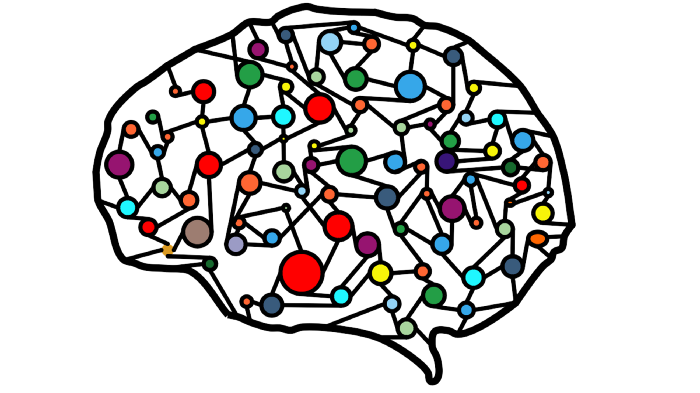
\includegraphics[width=3in]{pics/neural_network.png}
	\nbvspace[1]
	%\normalsize
	
	MASTER'S THESIS \\ 
	COPENHAGEN BUSINESS SCHOOL --- CAND.MERC.(MAT.)\\
    \nbvspace[1]
    DATE OF SUBMISSION: MAY 17 2021\\
    NUMBER OF PAGES: $\infty$ (-1000)
	
	\nbvspace[1]
\end{center}
\end{titlepage}
% --------------------------- Main document -------------------

\thispagestyle{empty}
\begin{center}
    \Large
    \textbf{Abstract}
\end{center}
\vspace{0.9cm}
THIS THESIS bla bla.. 
\\
\\
\keywords{Machine Learning, Neural Networks, Bayesian Neural Network, Deep Learning, TensorFlow, Markov Chain Monte Carlo, Python, Computational Statstics, Hamiltonian Monte Carlo, No-U-Turn Sampler, Bayesian Inference, Mathematics of Computing, Probability and Statistics, Bayesian Deep Learning, Stochastic Programming, PyMC3.}
\frontmatter
\thispagestyle{empty}
\begin{center}
    \Large
    \textbf{Resume}
\end{center}
\vspace{0.9cm}
Denne afhandling omhandler bla bla..
\\
\\
\keywords{Machine Learning, Neural Networks, Bayesian Neural Network, Deep Learning, TensorFlow, Markov Chain Monte Carlo, Python, Computational Statstics, Hamiltonian Monte Carlo, No-U-Turn Sampler, Bayesian Inference, Mathematics of Computing, Probability and Statistics, Bayesian Deep Learning, Stochastic Programming, PyMC3.}
\frontmatter

\section*{Acknowledgements}
\thispagestyle{empty}
Thanks to Peter Dalgaard. \\
Thanks to Eric J. Ma.\\
Thank to Rasmus Nielesen kollegie for a nice ping pong table.\\
Thanks to Caroline Enersen for very træstammer.


\tableofcontents \thispagestyle{empty} 
\listoffigures \thispagestyle{empty} \addcontentsline{toc}{chapter}{List of Figures}
\listoftables \thispagestyle{empty} \addcontentsline{toc}{chapter}{List of Tables}
\newpage
\nomenclature[N]{$a$}{A scalar (integer or real)}
\nomenclature[N]{$\boldsymbol{a}$}{A Vector}
\nomenclature[N]{$\boldsymbol{A}$}{A Matrix}
\nomenclature[N]{$\boldsymbol{I}_n$}{Identity matrix with $n$ rows and $n$ columns. Sometimes $n$ is omitted and implied by context}
\nomenclature[N]{$\text{a}$}{A scalar random variable}
\nomenclature[N]{$\mathbf{a}$}{A vector of random variables}
\nomenclature[N]{$\mathbf{A}$}{A matrix of random variables}


\nomenclature[S]{$\mathbb{A}$}{A set}
\nomenclature[S]{$\mathbb{R}$}{The set of real numbers}
\nomenclature[S]{$\{ 0,1 \}$}{The set containing 0 and 1}
\nomenclature[S]{$\{ 0,1, \dots, n \}$}{The set containing all integers between 0 and $n$}
\nomenclature[S]{$[a,b]$}{The real interval between and including $a$ and $b$}
\nomenclature[S]{$(a,b]$}{The real interval between $a$ and $b$ excluding $a$ but including $b$}


\nomenclature[I]{$a_i$}{Element $i$ of vector $\boldsymbol{a}$, with indexing starting at 1}
\nomenclature[I]{$A_{i,j}$}{Element $i,j$ of matrix $\boldsymbol{A}$}
\nomenclature[I]{$\text{a}_i$}{Element $i$ of the random vector $\mathbf{a}$}

\nomenclature[L]{$\boldsymbol{A}^\top$}{Transpose of matrix $\boldsymbol{A}$}



\nomenclature[P]{$P(\text{a})$}{A probability distribution over a discrete variable}
\nomenclature[P]{$p(\text{a})$}{A probability distribution over a continuous variable, or over a variable whose type has not been specified}
\nomenclature[P]{$\text{a} \sim P$}{Random variable $\text{a}$ has distribution $P$}
\nomenclature[P]{$\E_{\text{x} \sim P} \lrs{f(\text{x})}$  or $\E \lrs{f(\text{x})}$}{Expectation of $f(\text{x})$ with respect to distribution $P(\text{x})$. Sometimes subtext $\text{x} \sim P$ is omitted and implied by context}
\nomenclature[P]{$\text{Var}\lr{f(\text{x})}$}{Variance of $f(\text{x})$ under distribution $P(\text{x})$}
\nomenclature[P]{$\text{Cov}\lr{f(\text{x}, g(\text{x}))}$}{Covariance of $f(\text{x})$ and $g(\text{x})$ under distribution $P(\text{x})$}
\nomenclature[P]{$\mathcal{N} \lr{\boldsymbol{x};\boldsymbol{\mu}, \boldsymbol{\Sigma}}$}{Gaussian distribution over $\boldsymbol{x}$ with mean $\boldsymbol{\mu}$ and covariance $\boldsymbol{\Sigma}$}

\nomenclature[D]{$\mathbb{X}$}{A set of training examples}
\nomenclature[D]{$\mathbb{Y}$}{A set of target labels}
\nomenclature[D]{$\mathbb{H}$}{A set of hypothesis also called the hypothesis space}
\nomenclature[D]{S}{A data set or sample}
\nomenclature[D]{$\boldsymbol{x}^{(i)}$}{The $i$th (input) example from a dataset}
\nomenclature[D]{$y^{(i)}$ or $\boldsymbol{y}^{(i)}$}{The target associated with $\boldsymbol{x}^{(i)}$}
\nomenclature[D]{$\boldsymbol{X}$}{A $m \times n$ matrix with input example $\boldsymbol{x}^{(i)}$ in row $\boldsymbol{X}_{i,:}$}

\nomenclature[F]{$\mathbf{1} \lrs{\text{condition}}$}{Equal to $1$ if condition is true, 0 otherwise}
\nomenclature[F]{$\sigma(x)$}{Logistic sigmoid function $\frac{1}{1 + e^{-x}}$}

\printnomenclature

\mainmatter
%\setcounter{page}{1}

\chapter{Introduction}
\textcolor{red}{IN THIS THESIS BLALBLBLLBLBLBALLBLBS}
Tjek evt
\url{https://www.google.com/url?sa=t&rct=j&q=&esrc=s&source=web&cd=&ved=2ahUKEwiiyu3czKXwAhVkposKHRQzAG4QFjAEegQIAhAD&url=https%3A%2F%2Fosf.io%2Ffcmun%2Fdownload&usg=AOvVaw2gTiUF_IfbUDfBmxbtAaKR}

\clearpage
\section{Problem} \label{sec:problem}
This thesis aims to answer the following problem:
\begin{center}
    \textit{How do Markov chain Monte Carlo based Bayesian neural network perform regression and classification tasks and how is this different from non-Bayesian feedforward neural networks?}
\end{center}
\noindent
\\
This is done by answering the following research questions:
\begin{itemize}
    \item What is a supervised machine learning algorithm and how does it generally work?
    \item What is over- and underfitting and how do we prevent this in a supervised machine learning algorithm?
    \item What is gradient based optimization used for training a supervised machine learning algorithm, and how does the most common methods work?
    \item What is a feedforward neural network and how is it trained and regularized?
    \item What is Bayesian inference and how is it different from frequentist inference?
    \item What is Monte Carlo methods and how do they work?
    \item What is a Bayesian neural network and how does it work?
    \item What is a Markov chain Monte Carlo and how can we use it to sample?
    \item What is Hamiltonian Monte Carlo and how can we use it to sample?
    \item What are common used extensions of Hamiltonian Monte Carlo and how do they improve sampling?
    \item What role do priors play in Bayesian neural networks and how can we choose them properly? 
    \item How does non-Bayesian and Bayesian neural networks perform when used for predicting house prices in Boston using regression?
    \item How does non-Bayesian and Bayesian neural networks perform when used for predicting defaults on credit card loans using binary classification?
\end{itemize}
\clearpage

\section{Method}
We approach the questions posed in section \ref{sec:problem} using the positivist paradigm. Positivism is a philosophical theory that states that genuine knowledge exists and is structured in a specific way regardless of ones perspective of it. According to this theory, information is derived from sensory experienced, that is interpreted through reason and logic, which is reflected by our mathematical approach of examining Bayesian- and non-Bayesian neural networks. We evaluate these networks on data, which is in accordance to positivist view on verified data as empirical evidence. 
\\
\\
This thesis is mainly a theoretical examination of Markov chain Monte Carlo based Bayesian neural networks, with a focus on efficient sampling methods for these, and how they differ from non-Bayesian neural networks. We examine this by first clarifying basic theory for supervised machine learning algorithms, which is a category which neural networks belong. This will cover how to train such and algorithm and how to regularize it to prevent over- and underfitting. Afterwards numerous optimization algorithms used for training a supervised machine learning algorithm is covered. This provides the fundamentals for explaining a feedforward neural network, which is what we do then. We do this by covering it's general structures and various options for designing it. We also cover how it's trained using backpropagation and the previous covered optimization algorithms, and we cover how to do this with regularization techniques like early stopping.
\\
\\
With neural networks examined we have defined the model to which we take a Bayesian approach in Bayesian neural networks. Such networks are covered by first examining the difference in Bayesian and Frequentist (read non-Bayesian) learning. Then we examine Monte Carlo methods, which are often used in Bayesian inference models.
\\
\\
We then illustrate a simple Bayesian neural network, which we constructed to show how a such a network works, and to show the motivation for introducing more sophisticated sampling techniques when sampling from such networks. This naturally leads to an examination of Markov chain Monte Carlo methods, which provides the basics for such sampling methods. We use this knowledge to examine the Hamiltonian Monte Carlo method and the extensions of this in the pursuit of the most efficient sampling method for Bayesian neural networks. 
\\
\\
Afterwards we examine the consequence of choosing a prior and how to do so. As such choices often depend on the specific task, so we don't go into much detail. Instead we examine various general approaches and points to literature that supports these approaches. Finally we evaluate the Bayesian and non-Bayesian neural networks on real data. First a dataset for which we aim to predict house prices in Boston using regression and next a dataset on credit card defaults, where we try to predict defaults or non-defaults using binary classification. 


\section{Research delimitation}
To have a focused approach for answering our problem statement in section \ref{sec:problem}, we choose to not elaborate on certain subjects, as we deem them out of scope or answering this appropriately. As we focus on Markov chain Monte Carlo based Bayesian neural networks we don't examine other methods for using Bayesian inference in neural networks such as methods based on variational inference. We also refrain from examining too thoroughly the choice of priors, and we only cover the consequences of the choice and the most general methods, since the method of choosing a prior often depends on the data, the task and the researches prior knowledge of such. 
\\
\\
Different regularization methods \& other elaborate theory on non-bayesian neural networks \\
Markov Chains \\










\chapter{Machine Learning Basics}\label{sec:ml_basic}
This chapter provides a brief introduction to the fundamental theory of machine learning that is used throughout the rest of this thesis. 
Machine learning is the study of computer algorithms that learn by analyzing data. Most machine learning algorithms can be divided into the two categories of supervised learning and unsupervised learning. In the following, we will describe the informal distinction between these and the most common tasks used for supervised learning. As neural networks are considered supervised learning the following sections will focus only on theory for supervised learning algorithms.
\\
\\
We proceed to describe the challenge of finding patterns and generalizing these to new data while describing the various machine learning components such as capacity, loss functions and regularization. Most machine learning algorithms are based on the idea of minimizing a loss function by using an optimization algorithm to select the optimal parameters. One of the most common optimization algorithms used in the context of machine learning is called stochastic gradient descent. We cover this algorithm and its variants in in section \ref{sec:gradient_optimization}. We will later use the theory of stochastic gradient descent in combination with backpropagation in section \ref{sec:backprop} for describing learning in neural networks.



\section{Supervised Learning}
Supervised learning use labels on datapoints, which we call examples, as targets to create prediction rules for learning the label of new examples. In unsupervised learning useful properties of the data structure are learned without the model being provided with target labels to predict. However as mentioned by \cite{Goodfellow-et-al-2016} the distinction is not formally defined, since there is no objective way to determine whether a value is a feature or a target label.\\
\\
One example of a learning algorithm that is typically viewed as supervised is classic linear regression that uses examples $x$ and their labels $y$ to create a linear function to determine $y$-values of new examples $x$. An example of a learning algorithm that is typically viewed as unsupervised is $k$-means clustering, that divides a dataset into $k$ clusters based on distance. \\
\\
As neural networks and Bayesian neural networks use target labels to predict labels of new examples it is considered a supervised learning algorithm. Therefore the following chapter will only cover the machine learning basics of supervised algorithms. \\
\\
Typical tasks of supervised machine learning algorithms are:
\begin{itemize}
    \item Classification when the output space $\YY$ are labels. This is called binary classification in cases with only two possible labels. In this case the algorithm must learn to separate examples of these two labels. Binary labels (be it male/female, yes/no etc.) are typically translated to a numerical representation by letting $\YY = \{ \pm 1 \}$ or $\YY = \{0,1 \}$. When working with more than two, but still a finite number of labels, we call the task multiclass classification. Depending of the setting and amount of labels it can be preferable to use regression instead of multiclass classification.
    \item Regression when the output space $\YY = \mathbb{R}$. For example predicting someones weight could be modeled as a regression problem.
    \item Structured prediction when the output is not merely a number or a label, but a structured object. An example of this is machine translation where the input is a sentence in one language and the output a sentence in another language. 
\end{itemize}


\section{Loss Functions} \label{sec:loss_func}
In order to evaluate the performance of a supervised machine learning algorithm we use a quantitative measure called a loss function. The loss function is an encoding, of how much the algorithm should care about making certain kinds of mistakes, and it is based on this measure that the algorithm selects a hypothesis $h$ from a set of possible hypothesis $\mathbb{H}$ called the hypothesis space. A hypothesis (also called prediction rule) can be understood as a recipe, that the algorithm develops to perform its task. An example would be the weights $\boldsymbol{w}$ for performing the linear regression $\hat{y}^{(i)} = \boldsymbol{w}^\top \boldsymbol{x}^{(i)}$. Another example would be a specific range of values for a specific set of features for classification, like a set of RGB color-values to classify if an input-image is depicting an apple or a pear. We treat the hypothesis as a function $h\lr{\boldsymbol{x}^{(i)}}$ taking $\boldsymbol{x}^{(i)}$ as input and predicting $\hat{y}^{(i)}$. We define the loss function $\ell \lr{h \lr{\boldsymbol{x}^{(i)}}, y^{(i)}}$ as being the loss of predicting $h \lr{\boldsymbol{x}^{(i)}}$ when the target label is $y^{(i)}$.\\ 
\\
We want the algorithm to return the "best" hypothesis $h^*$, which in this context should be interpreted as the hypothesis that gives the least amount of expected loss on new samples $\lr{\mathbf{x}^{(i)}_{\text{new}}, \text{y}^{(i)}_{\text{new}}}$
\begin{equation*}
    L(h) \equiv \E \lrs{\ell \lr{h \lr{\mathbf{x}_{\text{new}}^{(i)}}, \text{y}_{\text{new}}^{(i)}}}
\end{equation*}
where the expectation is taken with respect to the data distribution $p_{\text{data}}$. If such a value is satisfyingly low, it means that $h^*$ is a useful tool for performing its task on new data. We define the optimal hypothesis formally by
\begin{equation*}
   h^* = \argmin_{h \in \mathbb{H}} L(h)
\end{equation*}
\\
\\
Common loss functions in regression are squared loss (also called L2 loss)
\begin{equation} \label{eq:mse}
    \ell\left(h\lr{\boldsymbol{x}^{(i)}}, y^{(i)} \right) = \lr{ h\lr{\boldsymbol{x}^{(i)}} - y^{(i)} }^2
\end{equation}
or absolute loss (also called L1 loss)
$$ \ell\left(h\lr{\boldsymbol{x}^{(i)}}, y^{(i)}\right) = \lra{h\lr{\boldsymbol{x}^{(i)}} - y^{(i)}}$$
These functions train the algorithm to create hypothesis that minimize the differences from the target labels.
\\
\\
A typical loss function used for binary classification is the zero-one loss 
$$ \ell\left(h\lr{\boldsymbol{x}^{(i)}}, y^{(i)}\right)=\1\left(h\lr{\boldsymbol{x}^{(i)}} \neq y^{(i)} \right)=\left\{\begin{array}{ll}
0, & \text { if } h\lr{\boldsymbol{x}^{(i)}}=y^{(i)} \\
1, & \text { otherwise }
\end{array}\right. $$
giving $0$ loss for when the predicted label $h\lr{\boldsymbol{x}^{(i)}}$ is equal to the true label $y^{(i)}$ and $1$ otherwise. This loss function trains the algorithm to generate hypothesis, that makes the least number of mistakes. 
\\
\\
Another classification loss function that do not just look at the predicted label, but at the probability of a certain prediction, is the cross-entropy loss or log-loss function. This assumes that instead of predicting the label, the hypothesis $h\lr{\boldsymbol{x}^{(i)}}$ generated by the model is a set of probabilities that each provide the probability that the example belong to each of the classes. For binary classification it is defined as
\begin{equation*}
    \ell\left(h\lr{\boldsymbol{x}^{(i)}}, y^{(i)} \right) = - \lr{y^{(i)} \log h\lr{\boldsymbol{x}^{(i)}} + \lr{1 - y^{(i)}}} \log \lr{1 - h\lr{\boldsymbol{x}^{(i)}}}
\end{equation*}
which is actually the negative log likelihood (so minimizing this maximizes likelihood, see section \ref{sec:mle} for maximum likelihood estimation) when assuming Bernoulli distribution for the targets. For multiclass classification this can be generalized by assuming multinomial distribution with one trail for the targets and taking the negative log likelihood. These probabilities are typically provided by a sigmoid or softmax function that maps $\mathbb{R} \rightarrow [0,1]$, these are explained further in section \ref{sec:feedforward_nn}. With a model, that outputs these probabilities as hypothesis, predictions are typically done by choosing the class for which the example has the highest probability of belonging to.
\\
\\
These are some of the convenient general choices, and there are many more. But such general loss functions is not necessarily the right choice for a particular application. For example if a company knows the exact monetary loss of packing a wrong item as a result of a misclassification happening in a robotic packaging system. Then it might be beneficial to use a table (perhaps formally written as a sum of indicatorfunctions) of the costs of packaging each of their items as a loss function instead of using the general ones found in the literature.



\section{Training \& Testing} \label{sec:train_val}
The central challenge in machine learning is making sure that the algorithm creates a hypothesis that perform well on new data that was not used in selecting the hypothesis. As mentioned in section \ref{sec:loss_func} this is done by minimizing $L(h)$, but as we do not know $p_\text{data}$ (if we did we wouldn't need the algorithm) we can not evaluate $L(h)$. We must instead approximate $L(h)$ by its empirical estimate 
\begin{equation*}
    \hat{L}(h,S)= \frac{1}{N} \sum_{i=1}^N \ell \lr{h\lr{\boldsymbol{x}^{(i)}}, y^{(i)}}
\end{equation*}
However when we select a hypothesis $\hat{h}^*_S$ in $\mathbb{H}$ based on empirical loss $\hat{L} \lr{h, S}$ then the loss of this hypothesis $\hat{h}^*_S$ becomes a biased estimate of $L(\hat{h}^*_S)$. This is because $\hat{h}^*_S$ is selected based on the minimum empirical error on $S$, so from the perspective of $\hat{h}^*_S$ new samples might not be interchangeable with samples in $S$, since including these new samples could result in a different hypothesis that minimizes the loss on $S$. \\
\\
To get an unbiased estimate of $L(\hat{h}^*_S)$ for evaluating a model it is common practice to split the sample set $S$ into a dataset $S_\text{train}$ and a test set $S_\text{val}$. One can then find the best hypothesis using the training set $h^*_\text{train}$ and afterwards use the test set for computation of $\hat{L}\lr{h^*_\text{train}, S_\text{val}}$ to evaluate the performance. Based on the assumption that new samples $\lr{\mathbf{x}^{(i)}_{\text{new}}, \text{y}^{(i)}_{\text{new}}}$ are distributed identically with the samples in $S_\text{val}$ then these new samples are exchangeable with the ones in $S_\text{val}$ from the perspective of $h^*_\text{train}$. This means that $\E \lrs{\ell \lr{h^*_\text{train} \lr{\boldsymbol{x}^{(i)}}, y^{(i)}}} = \E \lrs{\ell \lr{h^*_\text{train} \lr{\mathbf{x}^{(i)}_{\text{new}}}, \text{y}_{\text{new}}^{(i)}}}$ and therefore $\hat{L}\lr{h^*_\text{train}, S_\text{val}}$ is an unbiased estimate of $L(h^*_\text{train})$.

\subsection{Cross-Validation} \label{sec:cv}
Splitting a dataset into a training set and a test set can be problematic if the resulting test set is too small. Such a small test set will give rise to statistical uncertainties around the estimated average loss and will make it problematic to evaluate the model. When we have large dataset this is not a problem, but when we work with small datasets it can become a serious issue. \\
\\
To circumvent this issue is to use cross-validation. Cross-validation repeats the training and testing procedure on different randomly chosen splits of the original dataset. This enables us to use more examples for estimating the average test loss for the cost of computational power. This approach is also useful for choosing hyperparameters like regularization constants $\alpha$ covered in section \ref{sec:regularization}.\\
\\
A common method for cross-validation is the $K$-fold cross-validation that splits the dataset into $K$ non-overlapping and roughly equally sized subsets. On trial $i$ the $i$th subset is used as the test set while the rest $K - 1$ subsets are used in the training set. The test loss is then estimated by the cross-validation loss computed as the average test loss across the $K$ trials.\\
\\
One problem with this approach is however measuring the uncertainty since there is no unbiased estimators of the variance of the average error estimators as mentioned by \cite{Bengio04}, one must instead use approximations. Another discussed issue is how to choose the value for $K$. This problem does not have a clear answer but 5- or 10-fold cross-validation are generally recommended as a good compromise, see \cite{brieman_spector_1992} and \cite{kohavi_1992}.

\section{Overfitting \& Underfitting}
The average loss attained on the training set when selecting the best hypothesis $\hat{L}\lr{h^*_\text{train}, S_\text{train}}$ is what we will call the training error training loss. The average loss attained from the test set $\hat{L}\lr{h^*_\text{train}, S_\text{val}}$, used for testing the model, is what we will call test error or test loss.\\
\\
Having a low training error means that we have made a prediction rule that fit our training set well. Having a small gap between training and test error means that the prediction rule generalizes well on new data, which is why the test error is also sometimes called generalization error. These factors are what corresponds to underfitting and overfitting, which is used to measure performance of the model.\\
\\
Underfitting occurs when the model is not able to obtain a sufficiently low training error. This is seen in figure \ref{fig:regr_example} in the case of linear regression of degree 1, where the model fitted on the training data lies far from the training samples, meaning it must have a large mean squared error (MSE) on the training data. Overfitting occurs when the gap between the training error and test error is too large. This large gap indicates that the model faithfully reflects idiosyncrasies of the training data rather than the true underlying process generating the data. This can be seen in figure \ref{fig:regr_example} in the case of linear regression of degree 15, where the model lies very close to all of the training samples meaning it must have a very small MSE on the training data. But if we sample points from the true function we see that many of these will very likely lie far from the model, resulting in a large test error relative to the training error. Overfitting and underfitting are both something we want to avoid. \\
\\
We can control whether a model under- or overfits by changing its capacity. Capacity is a model's ability to learn a larger variety of hypothesis. A model with a low capacity might underfit the training set if it can not capture the structure of the data. A model with high capacity might overfit if it learns properties of the training set that is not representative of the test set. As an example we can increase the capacity of linear regression by allowing it to fit higher order polynomials, thus increasing the hypothesis space from which we draw prediction rules. This example is seen in figure \ref{fig:regr_example}, where we see that a low capacity causes underfitting while a very large capacity causes the model to overfit.

\begin{figure}
    \centering
    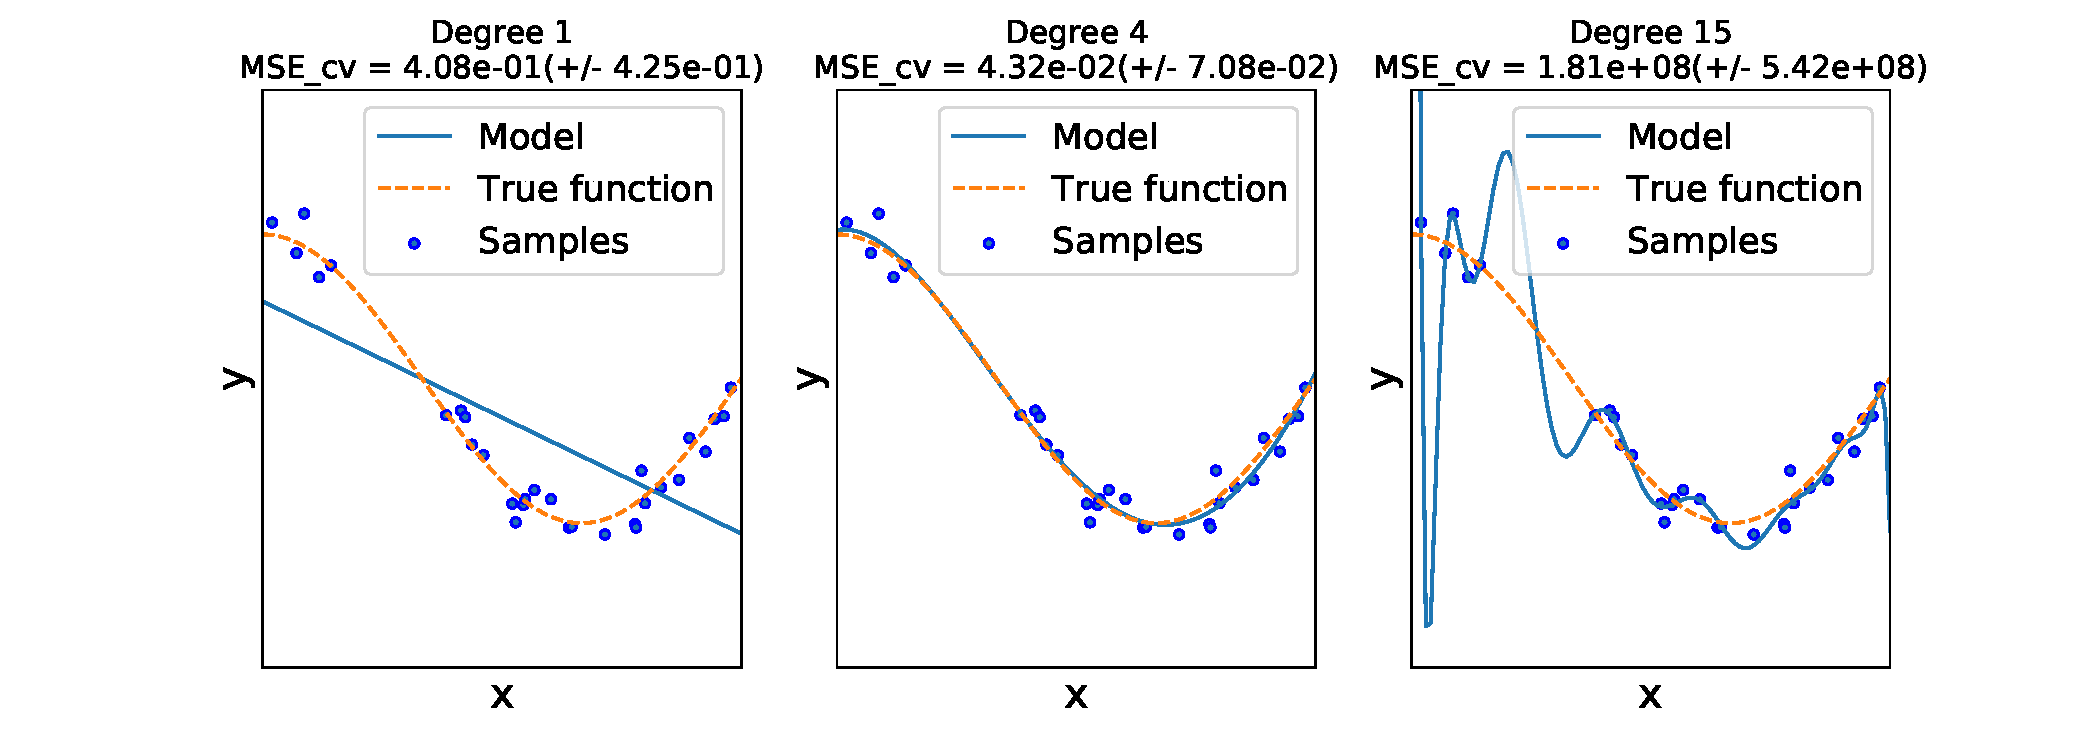
\includegraphics[width=\textwidth,keepaspectratio]{over_underfitting.pdf}
    \caption{Regression of different degree polynomials on a $\cos$ curve. We see that a linear regression of degree 1 is insufficient to fit the training set and is underfitting. A polynomial of degree 4 fits the curve almost perfectly while a polynomial of degree 15 learns the noise of the data and overfits. How well the different regressors generalize to a test set is evaluated quantitatively by calculating the mean squared error using the loss function in equation \ref{eq:mse} using 10-fold cross-validation. We see that this error is lowest when using 4-degree polynomial regression. Cross-validation is covered in section \ref{sec:cv}. The standard error of these losses are shown in the parenthesis. The Python code for producing this figure can be seen in appendix \ref{app:overfitting}.}
    \label{fig:regr_example}
\end{figure}
\noindent

\section{Regularization}\label{sec:regularization}
So far we have covered how to control over- and underfitting by changing a model's capacity. Another method is regularization which encodes the objective function with preferences for certain functions instead of excluding functions from the hypothesis space. The objective function is what we ask a machine learning algorithm to minimize, and has in the previous been synonymous with average loss. The hypothesis $h$ is what we will now embed in the choice of model parameters $\boldsymbol{\theta}$.\\
\\
A popular type of regularization is norm penalties, where a norm penalty function $\Omega(\boldsymbol{\theta})$ is added to the objective function  $J$ (which is usually average loss). Then the regularized objective function is
\begin{equation} \label{eq:reg_obj_func}
    \Tilde{J}(\boldsymbol{\theta}; \mathbf{X}, \mathbf{y}) = J(\boldsymbol{\theta}; \mathbf{X}, \mathbf{y}) + \alpha \Omega(\boldsymbol{\theta})
\end{equation}
where $\alpha \in [0, \infty]$ is a parameter chosen before minimizing $\Tilde{J}$, that controls how much the penalty term $ \Omega(\boldsymbol{\theta})$ contributes relatively to the objective function $J$. When $\alpha=0$ we have no regularization while larger values for $\alpha$ results in more regularization. In this way minimizing $ \Tilde{J}$ becomes a trade-off between fitting the training data and having small weights.\\
\\
A common norm penalty function is the L2 parameter norm penalty also known as weight decay $\Omega \lr{\boldsymbol{\theta}} = \frac{1}{2} \lra{\lra{\boldsymbol{\theta}}}_2^2$. L2 regularization is also known as ridge regression or Tikhonov regularization. In a regression setting $\boldsymbol{y} = \boldsymbol{x} \boldsymbol{w} + \boldsymbol{b}$, if we assume no bias parameter $\boldsymbol{b}$ and that model parameters are only weights $\boldsymbol{\theta} = \boldsymbol{w}$, the regularized objective function is defined by
\begin{equation} \label{eq:L2_reg}
    \Tilde{J}(\boldsymbol{\theta}; \mathbf{X}, \mathbf{y}) = J(\boldsymbol{\theta}; \mathbf{X}, \mathbf{y}) + \frac{\alpha}{2} \boldsymbol{\theta}^\top \boldsymbol{\theta}
\end{equation}
We can clearly see from this, that larger values of $\alpha$ punishes larger weights. \\
\\
A regularization method often used for neural networks is early stopping. We cover this method in section \ref{sec:early_stopping} providing a popular intuitive approach to regularization other than weight decay. 
\\
\\
There are many other techniques to reduce overfitting, which we will not cover. One such related type of regularization is norm penalties as constrained optimization problems where $\Omega \lr{\boldsymbol{\theta}}$ is constrained by some constant $k$ while seeking to minimize equation \ref{eq:reg_obj_func}. Another is data augmentation that increases the size of the training set by augmenting existing data and adding the augmented copy to the dataset. A last worthy mention, used specifically for neural networks, is dropout (\cite{srivastava2014dropout}), which regularize by ignoring a random set of network-nodes during training.

\section{Gradient Based Optimization}\label{sec:gradient_optimization}
Supervised machine learning algorithms are often based on learning parameters by minimizing a regularized loss function. This can be done for a differentiable convex loss function by minimizing its gradient, which is what we do in gradient based optimization. 

\subsection{Gradient Descent} 
Gradient descent is an algorithm suggested by \cite{Cauchy1847}. The algorithm is an iterative process of selecting parameters that decrease the gradient of the loss function $J(\boldsymbol{\theta},\boldsymbol{X},y)$. We will consider sampled examples from the sample space $\mathbb{X}$ and aim to estimate the model parameters $\boldsymbol{\theta}$. The goal is to minimize the loss function which we assume to be convex, so that the function is minimized where the gradient is zero
\begin{equation*}
    \nabla J(\boldsymbol{\theta},\boldsymbol{X},y)=\left[\frac{\partial J}{\partial\theta_1},\frac{\partial J}{\partial\theta_2},\ldots,\frac{\partial J}{\partial\theta_d}\right]=\boldsymbol{0}
\end{equation*}
The gradient tells us which direction that has the steepest slope on $J$, and we can thus change the model parameters such that we move in the opposite direction of where the gradient is pointing. This will bring us in the direction that locally decreases the objective function the fastest. In order to run the algorithm we need to initialize the model parameters $\boldsymbol{\theta}\equiv\boldsymbol{\theta}^0$, evaluate the objective function $J(\boldsymbol{\theta},\boldsymbol{X},y)$ and calculate the gradient respectively $\nabla J(\boldsymbol{\theta},\boldsymbol{X},y)$. Further we also need to specify a learning rate $\eta$, which affects the size of the step i.e. change in parameters in the direction of the negative gradient for each iteration. The model parameters are then updated iteratively by
\begin{equation*}
    \boldsymbol{\theta}^{(t+1)}=\boldsymbol{\theta}^{(t)}-\eta \nabla J(\boldsymbol{\theta}^{(t)},\boldsymbol{X},y)
\end{equation*}
This means, that when we are far away from optimum (large gradient) we are taking larger steps, but when we get closer to optimum (smaller gradient) we take smaller and smaller steps. The algorithm is not assured to reach a global minimum unless the loss function is strictly convex. \cite{bishop2007} mentions that in order to find a "good" minimum, we might be forced to run the algorithm multiple times, where we each time initialize with a randomly chosen starting point $\boldsymbol{\theta}^0$. 

\subsection{Stochastic Gradient Descent} \label{sec:sgd}
A widely popular and more computational feasible approach is to learn parameters using the stochastic gradient descent (SGD) algorithm. SGD is a stochastic approximation of the gradient descent algorithm described above, which replaces the gradient calculated on the entire dataset by an estimate calculated from a randomly selected subset of the data. This is useful when one faces high-dimensional optimization problems as it reduces the computational burden significantly (\cite{bottou2008tradeoffs}). Some authors append the term "mini-batch" to the algorithm name expect for the case where only one example has been used as a subset of the data.\\
\\
The pseudocode for SGD can be seen in algorithm \ref{alg:sgd}. Convergence and stopping criteria of descent algorithms have been studied extensively in the literature, and will not be discussed rigorously here. We will only provide some of the  most common stopping criteria found in software-packages. One is to stop when the norm of the gradient is beneath some threshold, $\norm{\nabla J \lr{\boldsymbol{\theta}^{(t-1)}}} < \epsilon$ another is when the decrease in norm of the gradient drops under some threshold, $\norm{\nabla J \lr{\boldsymbol{\theta}^{(t -1 )}}} - \norm{ \nabla J \lr{\boldsymbol{\theta}^{(t)}}} < \epsilon$. Most software also include a number of max iterations as a stopping criteria to prevent non-converging cases to run forever.\\
\begin{algorithm} \label{alg:sgd}
    \SetAlgoLined
    \KwInput{A dataset $S$}
    \KwInput{A learning rate $\eta$}
    \KwInput{Gradient function of objective function $\nabla J \lr{\boldsymbol{\theta}, \boldsymbol{x}, \boldsymbol{y}}$}
    \KwInput{Initial parameter vector $\boldsymbol{\theta}^{0}$}
    \KwOutput{Resulting parameters $\boldsymbol{\theta}$}
    initialize $\boldsymbol{\theta}\leftarrow \boldsymbol{\theta}^0$ \\
    \Repeat{stopping criteria is met}{
        $\text{pick randomly } S^\prime \in S$ \\
        $\boldsymbol{g} \leftarrow \frac{1}{\left|S^{\prime}\right|} \sum_{(\boldsymbol{x}, \boldsymbol{y}) \in S^{\prime}} \nabla_{\boldsymbol{\theta}} J\left(\boldsymbol{\theta},\boldsymbol{x},\boldsymbol{y}\right)$\\
        $\boldsymbol{\theta} \leftarrow \boldsymbol{\theta} - \eta \boldsymbol{g} $
    }
     \caption{Mini-Batch Stochastic Gradient Descent}
\end{algorithm}

\subsection{Stochastic Gradient Descent with Momentum}
One issue with SGD, shown by \cite{sutton1986}, is that it performs poorly with surfaces containing ravines, i.e places where the curvature is more steep in one dimension than in another, which is common around optima. In these cases SGD will oscillate across the slopes of the ravines while slowly making progress towards the optima. A method for accelerating the process towards the optima while dampening oscillation is introducing momentum. This is done by adding a fraction $\gamma$ of the update vector from time $t -1$, to the update vector for time $t$. Thus updating $\boldsymbol{\theta}$ by 
\begin{equation*}
    \begin{split}
        v_{t} &= \gamma v_{t -1} + \eta \nabla J \lr{\boldsymbol{\theta}^{(t)}} \\
        \boldsymbol{\theta}^{(t+1)} &= \boldsymbol{\theta}^{(t)} - v_t
    \end{split}
\end{equation*}
The momentum term increases for dimensions with gradients pointing in the same directions and reduces updates for dimensions where gradients change directions. This results in faster convergence and reduced oscillation.

\subsection{Adaptive Gradiant Algorithm (AdaGrad)}
Another possible improvement to SGD is by adapting the learning rate to the parameters, so that stepsize decreases as we perform each iteration. This makes it possible to move faster initially and afterwards slow down to avoid overstepping the optima, which will result in faster convergence. This method was proposed by \cite{duchi2011adaptive} with an SGD-extension called Adaptive Gradiant Algorithm (AdaGrad). AdaGrad performs the parameter-update by
\begin{equation*}
    \theta^{(t+1)}_i = \theta^{(t)}_i - \frac{\eta}{\sqrt{\varepsilon + \sum_{\tau = 1}^t \lr{\nabla J \lr{\theta_i}^{(t)}}^2}} \nabla J \lr{\theta_i}^{(t)}
\end{equation*}
making each parameters have its own learning rate $\frac{\eta}{\sqrt{\varepsilon + \sum_{\tau = 1}^t \lr{\nabla J \lr{\theta}^{(t)}}^2}}$, where $\varepsilon$ is a small number that ensures that we do not divide by $0$. As the sum of gradients increases with each step the learning rate decreases, which results in a smaller stepsize as the algorithm progresses.
\\
\\
Another upside to this approach, besides faster convergence, is that we do not need to manually tune the learning rate as it is now adapted. AdaGrad is also especially efficient when working with sparse data, as parameters for features that are often $0$ (infrequent features), can receive more impact-full updates (higher learning rate) without affecting the impact on features that are often non-zero (frequent features). Without adaptive learning rates for each parameter we might inefficiently have a learning rate that decreases too slowly for frequent features or too quickly for infrequent features.

\subsection{Root Mean Square Propagation (RMSprop)}
AdaGrad's weakness is that the learning rate eventually can become infinitesimally small, making it impossible for the algorithm to learn i.e. update the parameters further. The Root Mean Square Propagation (RMSprop) method suggested by \cite{Tieleman_Hinton2012} is an extension of AdaGrad, that seeks to overcome the weakness of AdaGrad's aggressive monotonically decreasing learning rate. RMSprob does this by replacing the sum of past gradients by an expectation of the gradient, thus updating parameters by
\begin{equation*}
    \theta^{(t+1)}_i = \theta^{(t)}_i - \frac{\eta}{\sqrt{\varepsilon + \E \lrs{\nabla J \lr{\theta_i^{(t)}}^2}}} \nabla J \lr{\theta_i^{(t)}}
\end{equation*}
where 
\begin{equation*}
    \E \lrs{\nabla J \lr{\theta_i^{(t)}}^2} = \lr{1 - \gamma}\nabla J \lr{\theta_i^{(t)}}^2 + \gamma \E \lrs{\nabla J \lr{\theta_i^{(t-1)}}^2}
\end{equation*}
which makes it possible for the learning rate to either increase or decrease for each epoch. RMSprob also efficiently define the sum of gradients recursively as a decaying average of past gradients instead of inefficiently storing all of the past gradients as in AdaGrad. The running average $\E \lrs{\nabla J \lr{\theta_i^{(t)}}^2}$ only depends on a hyperparameter-defined fraction $\gamma$ (similar to the momentum term), the previous average and the current gradient.


\subsection{Adaptive Moment Estimation (ADAM)} \label{sec:ADAM}
\cite{Kingma_Ba_2015} proposes an algorithm called Adaptive Moment Estimation (ADAM) which takes a similar approach to computing adaptive learning rate by storing an exponentially decaying average of past gradients $\boldsymbol{v}^{(t)}$ like RMSprop. ADAM however extends this idea by also keeping an exponentially decaying average of past gradients $\boldsymbol{m}^{(t)}$, that works similar to momentum. These components are calculated by 
\begin{equation*}
    \begin{split}
        \boldsymbol{m}^{(t)} &= \beta_1 \boldsymbol{m}^{(t-1)} + \lr{1- \beta_1}\nabla J \lr{\boldsymbol{\theta}^{(t)}}\\
        \boldsymbol{v}^{(t)} &= \beta_2 \boldsymbol{v}^{(t-1)} + \lr{1 - \beta_2}\nabla J \lr{\boldsymbol{\theta}^{(t)}}^2
    \end{split}
\end{equation*}
where $\nabla J \lr{\boldsymbol{\theta}^{(t)}}^2$ indicates the elementwise square $\nabla J \lr{\boldsymbol{\theta}^{(t)}} \odot \nabla J \lr{\boldsymbol{\theta}^{(t)}}$ and where $\boldsymbol{m}^{(t)}$ and $\boldsymbol{v}^{(t)}$ are estimates of the first moment and second moment of the time-$t$ gradient respectively, hence the name Adaptive Moment Estimation. 
The authors observed that as $\boldsymbol{m}^{(t)}$ and $\boldsymbol{v}^{(t)}$ are initialized as $\boldsymbol{0}$ they will be biased estimates. They counteract this bias by deriving the bias-corrected estimates
\begin{equation*}
    \begin{split}
        \hat{\boldsymbol{m}}^{(t)} &= \frac{\boldsymbol{m}^{(t)}}{1 - \beta_1^t}\\
        \hat{\boldsymbol{v}}^{(t)} &= \frac{\boldsymbol{v}^{(t)}}{1 - \beta_2^t}
    \end{split}
\end{equation*}
The parameters are then updated by 
\begin{equation*}
    \boldsymbol{\theta}^{(t+1)} = \boldsymbol{\theta}^{(t)} - \frac{\eta}{\sqrt{\hat{\boldsymbol{v}}^{(t)}} + \epsilon}\hat{\boldsymbol{m}}^{(t)}
\end{equation*}
The pseudocode for ADAM can be seen in algorithm \ref{alg:adam}.

\begin{algorithm}\label{alg:adam}
    \SetAlgoLined
    \KwInput{A dataset $S$}
    \KwInput{A learning rate $\eta$}
    \KwInput{Exponential decay rates for moment estimates $\beta_1, \beta_2 \in [0,1)$}
    \KwInput{Gradient function of objective function $\nabla J \lr{\boldsymbol{\theta}}$}
    \KwInput{Initial parameter vector $\boldsymbol{\theta}^{0}$}
    \KwOutput{Resulting parameters $\boldsymbol{\theta}$}
    initialize $\boldsymbol{\theta}\leftarrow \boldsymbol{\theta}^0$ \\
    initialize $\boldsymbol{m}^{(0)}, \boldsymbol{v}^{(0)}\leftarrow \boldsymbol{0}$\\
    initialize $t \leftarrow 0$\\
    \Repeat{stopping criteria is met}{
        $t \leftarrow t + 1$
        $\text{pick randomly } S^\prime \in S$ \\
        $\boldsymbol{g}^{(t)} \leftarrow \frac{1}{\left|S^{\prime}\right|} \sum_{(\boldsymbol{x}, \boldsymbol{y}) \in S^{\prime}} \nabla_{\boldsymbol{\theta}} J\left(\boldsymbol{\theta}^{(t-1)},\boldsymbol{x},\boldsymbol{y}\right)$\\
        $\boldsymbol{m}^{(t)} \leftarrow \beta_1 \boldsymbol{m}^{(t-1)} + (1 - \beta_1)\boldsymbol{g}^{(t)}$\\
        $\boldsymbol{v}^{(t)} \leftarrow \beta_2 \boldsymbol{v}^{(t-1)} + (1 - \beta_2)\boldsymbol{g}^{(t)^2}$\\
        $\hat{\boldsymbol{m}}^{(t)} \leftarrow \frac{\boldsymbol{m}^{(t)}}{1 - \beta_1^t}$\\
        $\hat{\boldsymbol{v}}^(t) \leftarrow \frac{\boldsymbol{v}^{(t-1)}}{1 - \beta_2^t}$\\
        $\boldsymbol{\theta}^{(t)} \leftarrow \boldsymbol{\theta}^{(t-1)} - \frac{\eta}{\sqrt{\hat{\boldsymbol{v}}^{(t)}} + \varepsilon} \hat{\boldsymbol{m}}^{(t)}$
    }
     \caption{ADAM (with mini-batch)}
\end{algorithm}






\chapter{Neural Networks}
Neural networks are machine learning algorithms inspired by the biological neural network that constitute the brain. The neural network is a collection of nodes called neurons that transmits and processes signals to and from other neurons connected to it, much like the biological neural network. The goal of a neural network is to approximate some function by learning parameters that results in the best approximation.
\\
\\
In this chapter we introduce the most common neural network, the feedforward neural network, in section \ref{sec:feedforward_nn}, which is the type of network we refer to throughout the dissertation, when we use the term neural network. In section \ref{sec:backprop} we examine a common method for training a neural network called backpropagation and in sections \ref{sec:early_stopping} and \ref{sec:dropout} we introduce some popular methods of regularizing neural networks to avoid overfitting. 

\section{Feedforward Neural Networks} \label{sec:feedforward_nn}
The most simple neural networks are called feedforward neural networks or multilayer perceptrons (MLPs). They are called feedforward as information flows in one direction through the neurons. The neurons are typically arranged in layers to indicate which neurons receive and sends data to which neurons. These layers are typically vector-valued with each element of the vector playing the role as a neuron. As such one can describe a neural network as a chain of functions. Say we have 3 layers, then the neural network is $f(\mathbf{x}) = f^{(3)}\lr{f^{(2)}\lr{f^{(1)}\lr{\mathbf{x}}}}$, with $f^{(1)}$ being the first layer to pass the data, $f^{(2)}$ the second layer and so on. The final layer is called the output layer, while the intermediate layers, that don't directly show their output to the user, are called hidden layers. \\
\\
A feedfoward neural network is shown in figure \ref{fig:mlp} where the data flows from the input layer through 2 hidden layers and finally to the output layer. While the number of neurons in the input layer and output layer depends on example and label dimensions, the number of neurons in the hidden layers and also the number of hidden layers are a design decision chosen by the architect. \\
\\
The data is sent through these layers by multiplying the inputs with weights $\boldsymbol{w}$, adding a bias $\boldsymbol{b}$ and finally applying an activation function $g$ to the result. An activation function is a non-linear function that makes it so we don't just pass linear transformations of the examples through the network, so that we can actually learn non-linear functions. Activation functions come in many different kinds, some of the most popular can be seen in figure \ref{fig:act_funcs}. For a network with 2 hidden layers the result of the first hidden layer is $f^{(1)}\lr{\boldsymbol{X}} = g_1 \lr{\boldsymbol{X} \boldsymbol{w}_1 + \boldsymbol{b}_1}$ and the result of the second hidden layer is $f^{(2)} \lr{f^{(1)}\lr{\boldsymbol{X}}} = g_2 \lr{f^{(1)}\lr{\boldsymbol{X}} \boldsymbol{w}_2 + \boldsymbol{b}_2}$. The subscripts indicate that the activation functions, weights and biases are unique for each layer. Lastly the result of the output layer is $f^{\text{out}} \lr{f^{(2)} \lr{f^{(1)}\lr{\boldsymbol{X}}}} = g_3 \lr{f^{(2)} \lr{f^{(1)}\lr{\boldsymbol{X}}} \boldsymbol{w}_3 + \boldsymbol{b}_3}$. Sometimes the biases are omitted, as they can be represented in the weight vector for an example-matrix that are padded with a column of ones. \\
\\
While the choice of activation function are chosen as a design decision by the architect for the hidden layers, the activation function for the output layer are chosen by the learning task. If the neural network are to do regression then typically a linear activation function or none at all are chosen for the output layer as the label space for regression is the real numbers. However for binary classification a sigmoid-function is used and for multiclass classification then a softmax-function is used, as these map real values to the interval [0,1] and thus provides valid probabilities for belonging to a specific class. These activation functions among the ones shown in figure \ref{fig:act_funcs} are defined as follows:\\
\\
Logistic sigmoid:
\begin{equation*}
    g(x) = \sigma(x) \equiv \frac{1}{1 + e^{-x}}
\end{equation*}
\textcolor{red}{Add text on how this is used as an output-activation function for performing binary classification by mapping $\mathbb{R} \rightarrow [0,1]$, and add text on how the softmax function is used as an output-activation function for multiclass classification.}\\
Hyperbolic tangens:
\begin{equation*}
    g(x) = \tanh \lr{x} \equiv \frac{e^x - e^{-x}}{e^x + e^{-x}}
\end{equation*}
Rectified linear unit (ReLU):
\begin{equation} \label{eq:relu}
    g(x) = \max \lr{0, x}
\end{equation}
Exponential linear unit (ELU):
\begin{equation*}
    g(x) = \begin{cases}
    a & a \geq 0 \\
    \alpha \lr{e^a - 1} & a < 0
    \end{cases} \quad \text{for } \alpha > 0
\end{equation*}
Step:
\begin{equation*}
    g(x) = \mathbf{1}_{x > 0}
\end{equation*}



\begin{figure}
    \centering
    \begin{neuralnetwork}[height = 4]
        \newcommand{\x}[2]{$x_#2$}
        \newcommand{\y}[2]{$\hat{y}_#2$}
        \newcommand{\hfirst}[2]{\small $h^{(1)}_#2$}
        \newcommand{\hsecond}[2]{\small $h^{(2)}_#2$}
        \inputlayer[count=3, bias=false, title=Input\\layer, text=\x]
        \hiddenlayer[count=4, bias=false, title=Hidden\\layer 1, text=\hfirst] \linklayers
        \hiddenlayer[count=3, bias=false, title=Hidden\\layer 2, text=\hsecond] \linklayers
        \outputlayer[count=2, title=Output\\layer, text=\y] \linklayers
    \end{neuralnetwork}
    \caption{Feedforward neural network with 2 hidden layers and arrows indicating where neurons feed their data.}
    \label{fig:mlp}
\end{figure}

\begin{figure}
    \centering
    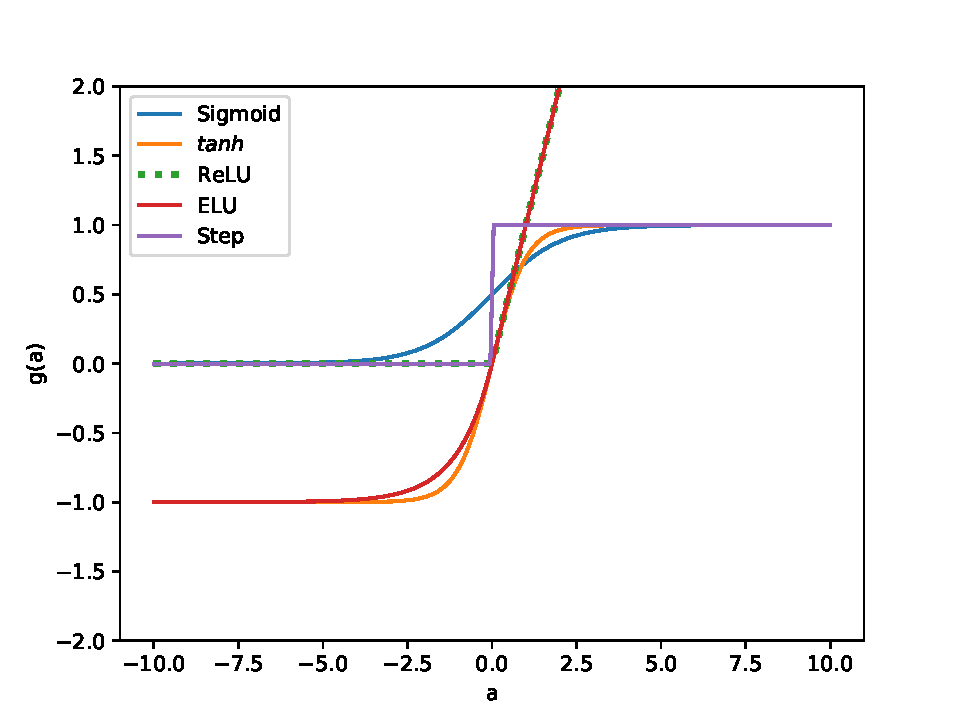
\includegraphics[width=\textwidth,height=\textheight,keepaspectratio]{pics/act_func_fig.pdf}
    \caption{Plot of some of the most used activation functions.}
    \label{fig:act_funcs}
\end{figure}


\section{Backpropagation} \label{sec:backprop}
As mentioned in section \ref{sec:train_val} we seek to find the hypothesis $\hat{h}^*_S$ that minimizes our loss empirical loss. \textcolor{red}{Mention here that we will collect the bias and weights in a parameter vector $\boldsymbol{\theta}$ for simplicity as we instead of added this bias can put it in the weight-vector if we pad each example with a column of 1's, which makes $\boldsymbol{x}\boldsymbol{w}+\boldsymbol{b} = \boldsymbol{x}_{\text{padded}} \boldsymbol{\theta}$ - replace w by theta in the following and in the algorithms 3 and 4.} In the case of neural networks (with omitted bias terms) $\hat{h}^*_S$ are the weights used in each neuron as described in section \ref{sec:feedforward_nn}. To obtain these optimal weights we train the neural network by minimizing the gradient of the (perhaps regularized) loss function $J$ with respect to the weights. To learn these weights we use a minimization algorithm like stochastic gradient descent described in section \ref{sec:sgd}. However the gradient of the loss function is not readily available in neural networks as we have to trace back the information back through the network that produced $\hat{y}$ for which we calculate the loss. The solution is an algorithm proposed by \cite{Rumelhart:1986a} called back-propagation or backprop for short.\\
\\
Back-propagation uses the chain rule of calculus, which states that
\begin{equation*}
    \frac{d \, f\lr{g\lr{x}}}{d \, x} = \frac{d \, f\lr{g\lr{x}}}{d \, g \lr{x}} \frac{d \, g\lr{x}}{d \, x}
\end{equation*}
for a real number $x$ and functions $g$ and $f$. This rule can be generalized for a vector $\boldsymbol{x} \in \mathbb{R}^m$
\begin{equation*}
    \frac{\partial f\lr{g\lr{\boldsymbol{x}}}}{\partial x_i} = \sum_j \frac{\partial f\lr{g\lr{\boldsymbol{x}}}}{\partial g(x_j)} \frac{\partial g(x_j)}{\partial x_i}
\end{equation*}
where $g: \mathbb{R}^m \rightarrow \mathbb{R}^n$ and $f: \mathbb{R}^n \rightarrow \mathbb{R}$. In a neural network with 1 hidden layers we find the gradient of the loss function $J(\boldsymbol{w})$ (with $\boldsymbol{X}$ and $\boldsymbol{y}$ as implicit inputs to keep notation uncluttered) by
\begin{equation} \label{eq:loss_grad}
    \nabla J\lr{\boldsymbol{w}} = \begin{pmatrix}
    \frac{\partial J\lr{f^{\text{out}} \lr{f^{(1)}\lr{\boldsymbol{w}}}}}{\partial w_1} \\
    \vdots\\
    \frac{\partial J\lr{f^{\text{out}} \lr{f^{(1)}\lr{\boldsymbol{w}}}}}{\partial w_m}
    \end{pmatrix}
\end{equation}
where each element in found by
\begin{equation} \label{eq:loss_grad_element}
    \frac{\partial J\lr{f^{\text{out}} \lr{f^{(1)}\lr{\boldsymbol{w}}}}}{\partial w_i} = \sum_j \frac{\partial J\lr{f^{\text{out}} \lr{f^{(1)}\lr{\boldsymbol{w}}}}}{\partial f^{\text{out}} \lr{f^{(1)}\lr{w_j}}} 
    \frac{\partial f^{\text{out}} \lr{f^{(1)}\lr{w_j}}}{\partial f^{(1)}\lr{w_j}} 
    \frac{\partial f^{(1)}\lr{w_j}}{\partial w_i}
\end{equation}
This provides the fundamentals to understand how the gradient is computed in practice.
First a vector of weights (perhaps chosen by an update of stochastic gradient descent) is sent through the network as shown by algorithm \ref{alg:forward_prop} to provide a loss value. This is called forward-propagation. Then the gradient in equation \ref{eq:loss_grad} is computed using the relation in equation \ref{eq:loss_grad_element} by back-propagation as shown in algorithm \ref{alg:back_prop}. The result of the backpropagation algorithm is gradients on the weights (and biases) that can be directly used for learning the weights that minimizes the gradient on the loss in a stochastic gradient descent algorithm as the one shown in algorithm \ref{alg:sgd}.\\
\\
Some activation functions like the ReLU-function $g(x) = \max \lr{0, x}$ are not differential, which might sound problematic for backpropagation and gradient based learning. However, as mentioned by \cite{Goodfellow-et-al-2016}, gradient descent still performs well enough for these models, partly because training algorithms usually don't arrive at a local minimum of the loss function. This means that we don't expect to get a gradient of $\boldsymbol{0}$, and therefore we can accept that the minimum of the loss function corresponds to points with an undefined gradient. Furthermore \cite{Goodfellow-et-al-2016} mentions that most software return one of the one-sided derivatives, which can be heuristically justified since a computer is subject to numerical error anyway. \\
\\
\textcolor{red}{Perhaps add text and figure on symbol-to-symbol differentiation as in goodfellow p. 214 and fig. 6.10.}

\begin{algorithm}\label{alg:forward_prop}
\SetAlgoLined
\KwInput{Number of layers, $l$}
\KwInput{The weight vectors of each layer $\boldsymbol{w}^{(i)}, i \in \lrc{1, \dots, l}$}
\KwInput{The activation functions of each layer, $g^{(i)}, i \in \lrc{1, \dots, l}$}
\KwInput{The example to process, $\boldsymbol{x}$}
\KwInput{The target label for the example, $\boldsymbol{y}$}
\KwOutput{The loss on the example, $J = L\lr{\boldsymbol{\hat{y}}, \boldsymbol{y}} + \lambda \Omega \lr{\boldsymbol{\theta}}$}
 initialize $\boldsymbol{h}^{(0)} = \boldsymbol{x}$ \\
\For{$k = 1, \dots, l$}{
    $\boldsymbol{a}^{(k)} = \boldsymbol{w}^{(k)} \boldsymbol{h}^{(k-1)}$ \\
    $\boldsymbol{h}^{(k)} = g^{(k)} \lr{\boldsymbol{a}^{(k)}}$ \\
}
$\hat{\boldsymbol{y}} = \boldsymbol{h}^{(l)}$ \\
$J = L\lr{\boldsymbol{\hat{y}}, \boldsymbol{y}} + \lambda \Omega \lr{\boldsymbol{\theta}}$ \\
 \caption{Forwardpropagation through a neural network and the computation of the cost function. For simplicity this demonstration uses only a single input example $\boldsymbol{x}$, in practice one typically uses a minibatch of examples. We have also omitted the bias terms for simplicity, as these can be part of the weights $\boldsymbol{w}^{(i)}$ with an example $\boldsymbol{x}$ padded with a column of 1's. The collection of weights are denoted by $\boldsymbol{\theta}$.}
\end{algorithm}

\begin{algorithm}\label{alg:back_prop}
\SetAlgoLined
\KwInput{Same variables as forwardpropagation in algorithm \ref{alg:forward_prop}}
\KwOutput{The gradient of the regularized loss function on the weights, $ \boldsymbol{d} = \nabla_{\boldsymbol{w}}J$}
Perform forward propagation as per algorithm \ref{alg:forward_prop}\\
Computation of the loss-gradient on the output layer:\\
$\boldsymbol{d} \leftarrow \nabla_{\hat{\boldsymbol{y}}} J =  \nabla_{\hat{\boldsymbol{y}}} L\lr{\hat{\boldsymbol{y}}, \boldsymbol{y}}$ \\
\For{$k = l, l-1, \dots, 1$}{
    $\boldsymbol{d} \leftarrow \nabla_{\boldsymbol{a}^{(k)}}J = \boldsymbol{d} \odot g^{(k)'} \lr{\boldsymbol{a}^{(k)}}$\\
    $\nabla_{\boldsymbol{w}^{(k)}} J = \boldsymbol{d} \boldsymbol{h}^{(k-1)^\top} + \lambda \nabla_{\boldsymbol{w}^{(k)}} \Omega \lr{\boldsymbol{\theta}}$\\
    $\boldsymbol{d} \leftarrow \nabla_{\boldsymbol{h}^{(k-1)}} J = \boldsymbol{w}^{(k)^\top} \boldsymbol{d}$\\
}
\caption{Back-propagation, \textcolor{red}{Understand this and comment on how it relates to equation \ref{eq:loss_grad_element}}}
\end{algorithm}

\section{Early Stopping} \label{sec:early_stopping}
\cite{Goodfellow-et-al-2016} mentions that when we have large models with sufficient capacity to overfit, then we often observe that training error decreases steadily over time, while validation error begins to rise again at some point before ending the training, and that this happens very reliably. This mean that we obtain a better model if we stop training and return the parameters at the point with the lowest validation error. This is the concept of regularizing using early stopping. The algorithm terminates training when no parameters have improved the validation-error over some pre-specified number of iteration called the patience, $p$. The measure of improvement can be controlled by a hyperparameter $\delta$, so that we only constitute an improvement if the decrease in validation error is more than $\delta$. The parameters $\boldsymbol{\theta}$ used for calculating the loss are provided by a training algorithm like ADAM from section \ref{alg:adam} using back-propagation from section \ref{sec:backprop}, while the loss is provided by the network-output for these parameters and the chosen loss function. This procedure is specified more formally in algorithm \ref{alg:es}.

\begin{algorithm}\label{alg:es}
\SetAlgoLined
\KwInput{The number of steps between evaluations, $n$}
\KwInput{The patience parameter i.e. the number of times of observing worsening validation error before terminating, $p$}
\KwInput{The measure of improvement, $\delta$}
\KwOutput{Parameters when terminating $\boldsymbol{\theta}^{*}$, training step when terminating $i^{*}$}
    initialize $i, j \leftarrow 0$ \\
    initialize $v \leftarrow \infty$\\
    Let $\boldsymbol{\theta}_0$ be the initial parameters\\
    $\boldsymbol{\theta}^* \leftarrow \boldsymbol{\theta}_0$\\
    $i^* \leftarrow i$\\
    \While{$j < p$}{
        Update $\boldsymbol{\theta}$ by running the training algorithm for $n$ steps\\
        $i \leftarrow i + n$\\
        $v' \leftarrow \hat{L}\lr{S_{\text{val}}, \boldsymbol{\theta}}$\\
        \If{$v' < v - \delta$}{
            $j \leftarrow 0$\\
             $\boldsymbol{\theta}^* \leftarrow \boldsymbol{\theta}$\\
            $i^* \leftarrow i$\\
            $v \leftarrow v'$\\
            \Else{
                $j \leftarrow j +1$
            }
        }
    }
 \caption{Early stopping}
\end{algorithm}

%One can think of early stopping as a hyperparameter selection algorithm that chooses the number of training steps for the training algorithm. The only significant cost of choosing this parameter automatically with early stopping is running the evaluation of the validation error periodically during training. However this can be done in parallel to the training process, as in Tensorflow where one can run parallel on the GPU. An additional cost is the need to maintain a copy of the optimal parameters, but this is negligible according to \cite{Goodfellow-et-al-2016} since they are written to infrequently and never during the training-algorithm, and since they can preferable be stored in a slower and larger form of memory like in host memory or disk drive. \\
%\\
%\cite{bishop1995} and \cite{sjoberg_ljung1995} argues that early stopping has the effect of restricting the optimization procedure to a small volume of parameter space in the neighborhood of the initial parameter value. \cite{Goodfellow-et-al-2016} shows with a simple linear model with a quadratic error function and simple linear descent how early stopping is equivalent to $L^2$ regularization in equation \ref{eq:L2_reg}, but that early stopping has the advantage of automatically determining the correct amount of regularization while $L^2$ regularization requires many training experiments with different values of its hyperparameter $\alpha$. 

\section{Dropout} \label{sec:Dropout}
\chapter{Bayesian Neural Networks}


\section{Bayesian versus frequentist views of learning}\label{sec:bayesian_stat}
In this section we will introduce two concepts of statistical inference. In inferential statistics, the goal is to infer something about a population from data which comes from a sample taken from the population. There are two main approaches in statistical inference, the Bayesian and the Frequentistic paradigm.\\ 
\\
The ideas behind Bayesian statistics goes back to the 18th century and is named after Thomas Bayes (\cite{stigler1986history}). The theory considers probability to reflect uncertainties and belief. Learning is performed by simple applications of rules of probability in particular Bayes' Rule. The results of Bayesian learning are probability distributions over all unknown quantities. On the other hand the conventional frequentistic methodology is to consider the model parameters $\boldsymbol{\theta}$ as fixed but unknown, while the point estimate $\hat{\boldsymbol{\theta}}$ is a random variable, as it is a function of the data set which is assumed to be random and conclusions are made by emphasizing the frequency of the data.
\\
\\
To illustrate the difference between these two methods in more detail, we will consider an example which is often used in the litterateur when comparing these two paradigms, it involves a simple coin toss. There is an uncertainty in this experiment regarding the outcome, will the coin come up heads or tails. This uncertainty can be expressed by the coins probability $p$ of landing on heads, this also often referred to as the bias of the coin. Since the properties of the coin is not known beforehand, we do not know what the exact probability of the coin landing on heads, it could be a fair coin and thus the probability would be $p=\frac{1}{2}$ or it could be an unbalanced coin $p\neq \frac{1}{2}$.\\
\\
A Bayesian statistician would express this uncertainty by a probability distribution over possible values of the unknown probability, and she would then update the distribution as more observations becomes known. On the other hand a frequentist, would find the introduction of a distribution over parameter weights as pure nonsense. The frequentist would instead flip the coin a given number of times to form a data set, and choose some estimator, for the unknown probability $p$ which would be most consistent with the data, an obvious choice would be the relative frequency of heads in the past coin tosses. For example if we flip the coin $n$ times and it has come up heads 70\% of the time, the frequentist would say that this coin is unbalanced whereas the Bayesian would say that it surely looks like the coin is unbalanced, and then update her belief about the coin as more and more flips are repeated. In the next section we will introduce these two paradigms in a more formal way.


\subsection{Maximum Likelihood Estimation}
Let us now consider a data set $\mathbf{X}$, with $n$ examples $x^{(1)}, x^{(2)},\ldots x^{(n)}$ drawn independently form the true but unknown distribution. We let
$L(\mathbf{X};\boldsymbol{\theta})\equiv p(\mathbf{X};\boldsymbol{\theta})$, be parametric family of probability distributions, with parameter $\boldsymbol{\theta}$, which is called the likelihood function. A frequentist is as described earlier trying to find an estimate of the true parameter that have generated the data, we call such an estimate a point estimate and denote $\hat{\boldsymbol{\theta}}$ to separate it from the true parameter. A point estimate can be viewed as a function of data $\hat{\boldsymbol{\theta}}=g(x^{(1)}, x^{(2)},\ldots x^{(n)})$ which is drawn from a random process and thus $\hat{\boldsymbol{\theta}}$ is a random variable.
In most cases of frequentistic inference a point estimate is found by maximizing the likelihood and thus called the maximum likelihood estimate (MLE)
\begin{equation*}
\begin{split}
        \boldsymbol{\boldsymbol{\theta}}_{\text{MLE}}&=\argmax_{\boldsymbol{\theta}}{L(\mathbf{X};\boldsymbol{\theta})}\\
        & = \argmax_{\boldsymbol{\theta}}{\prod^n_{i=1}p(x^{(i)},\boldsymbol{\theta})}
\end{split}
\end{equation*}
It is often more convenient to maximize a sum instead of a product, not only is it easier to handle sums when differentiating but it also helps stabilize the calculations numerically (\cite{Goodfellow-et-al-2016}), thus we take the log of the likelihood function to obtain the log-likelihood function $\ell(\mathbf{X};\boldsymbol{\theta})\equiv \ln{p(\mathbf{X};\boldsymbol{\theta})}$,
\begin{equation*}
\begin{split}
        \boldsymbol{\boldsymbol{\theta}}_{\text{MLE}}&=\argmax_{\boldsymbol{\theta}}{\ell(\mathbf{X};\boldsymbol{\theta})}\\
        &=\argmax_{\boldsymbol{\boldsymbol{\theta}}}{\sum^n_{i=1}\ln{p(x^{(i)},\boldsymbol{\theta})}}
\end{split}
\end{equation*}
and since the logarithm is a monotonic-increasing function, optimizing the log-likelihood is equivalent to optimizing the likelihood. \\
\\
There is two main reasons on why maximum likelihood is considered the preferred estimator to use by frequentist in statistics and machine learning, the MLE is consistent and efficient. We say that an estimator $\hat{\boldsymbol{\theta}}$ is consistent if it converges in probability to the true parameter. That is
\begin{equation*}
    \lim_{n \rightarrow \infty} p\left(\mid\hat{\boldsymbol{\theta}}-\boldsymbol{\theta}\mid > \epsilon\right)=0
\end{equation*}
for all $\epsilon>0$ and an efficient estimator is an estimator that estimates the true parameter of interest in some best possible manner. \\
\\
When data is small, the MLE is often prone to overfitting and regularization methods such as penalized maximum likelihood are applied (see e.g \cite{hastie01statisticallearning}).\\
\\
The sum of squared error in equation \ref{eq:mse} can be justified theoretically by the use of maximum likelihood with a Gaussian likelihood.
To see this consider that we have regression model that output $f(\mathbf{X};\boldsymbol{\theta})=\boldsymbol{\theta}^\top\mathbf{X}$, with real-valued targets $y^{(i)}$ and the likelihood defined as the conditional distribution of $y^{(i)}$ given the data $\mathbf{X}$ and the parameters $\boldsymbol{\theta}$ is gaussian with mean given by the regression output $\hat{y}\equiv f(\mathbf{X};\boldsymbol{\theta})$ and standard deviation $\sigma$, we can thus write
\begin{equation*}
    L(\mathbf{X};\boldsymbol{\theta})=\prod_{i=1}^{N} p\left(y^{(i)} \mid \mathbf{X}^{(i)} ; \boldsymbol{\theta}\right)=\prod_i\frac{1}{\sqrt{2\pi\sigma}}\exp\left(-(\hat{y}^{(i)}-y^{(i)})^2/2\sigma^2\right)
\end{equation*}
Next we take the
logarithm of the likelihood function which gives us the log-likelihood function
\begin{equation*}
\begin{split}
        \ell(\mathbf{X};\boldsymbol{\theta})&=\sum_i\ln\frac{1}{\sqrt{2\pi\sigma}}\exp\left(-(\hat{y}^{(i)}-y^{(i)})^2/2\sigma^2\right)\\
        &=-\frac{n}{2} \ln \sigma^{2}-\frac{n}{2} \ln (2 \pi)-\frac{1}{2 \sigma^{2}} \sum_{i}\left(\hat{y}^{(i)}-y^{(i)}\right)^{2}
\end{split}
\end{equation*}
note that $-\frac{n}{2} \ln \sigma^{2}-\frac{n}{2} \ln (2 \pi)$ does not depend on the model parameters $\boldsymbol{\theta}$ and can thus be omitted when we are maximizing. Maximizing the log-likelihood is the same as minimizing the negative log-likehood, thus we can write 
\begin{equation*}
\begin{split}
        \min_{\boldsymbol{\boldsymbol{\theta}}}{- \ell(\mathbf{X};\boldsymbol{\theta})}=\frac{1}{2 \sigma^{2}} \sum_{i}\left(\hat{y}^{(i)}-y^{(i)}\right)^{2}
\end{split}
\end{equation*}
and since $\frac{1}{2 \sigma^{2}}$ does not depend on $\boldsymbol{\theta}$ either, we can see that minimizing the negative log-likelihood is the same as minimizing the sum of squared error term in equation \ref{eq:mse}.\\
\\
\textcolor{red}{SHOW THAT MAXIMUM LIKELIHOOD IS THE SAME AS CROSS-ENTROPY??}




\subsection{Bayesian learning and prediction}
As we discussed in the introduction to this section: where the frequentist considers the parameter value $\boldsymbol{\theta}$ as fixed but unknown, and the point estimator $\hat{\boldsymbol{\theta}}$ as random variable, the Bayesian perspective on statistics is quite different, since it considers the dataset as being fixed and observable and thus not at all random. On the other hand the true parameter $\boldsymbol{\theta}$ is unknown and thus considered a random variable. \\
In Bayesian modelling, we begin with defining a prior distribution $p(\boldsymbol{\theta})$ over the parameters. This prior distribution expresses our initial view on the parameters, before any data has been observed. When data becomes available, we update our prior distribution to a posterior distribution. The posterior distribution is defined by Bayes' Rule, 
\begin{equation*}
         p(\boldsymbol{\theta}|\mathbf{X},\mathbf{y})=\frac{p(\boldsymbol{\theta})p(\mathbf{X},\mathbf{y}|\boldsymbol{\theta})}{p(\mathbf{X},\mathbf{y})}
\end{equation*}
and it combines the information about the data, that comes from the likelihood function $p(\mathbf{X},\mathbf{y}|\boldsymbol{\theta})$, with the a priori information given by the prior distribution. $p(\mathbf{X},\mathbf{y})$ is called the model evidence and can be interpreted as a normalizing constant given as $p(\mathbf{X},\mathbf{y})=\int p(\mathbf{X},\mathbf{y}\mid \boldsymbol{\theta})p(\boldsymbol{\theta})d\boldsymbol{\theta}$.
We often ignore the normalizing constant and simply writes, 
\begin{equation} \label{eq:posterior}
    p(\boldsymbol{\theta}|\mathbf{X},\mathbf{y})\propto p(\boldsymbol{\theta})p(\mathbf{X},\mathbf{y}|\boldsymbol{\theta})
\end{equation}
An important quality of the Bayesian method, is that is uses a full distribution over the parameters $\boldsymbol{\theta}$ to make predictions. Let us for example consider the case where we have observed a sample consisting of $n$ examples $\mathbf{X}=\boldsymbol{x}^{(1)}, \boldsymbol{x}^{(2)},\ldots, \boldsymbol{x}^{(n)}$, to predict an unobserved label $\boldsymbol{y}^{(n+1)}$ for a new example $\boldsymbol{x}^{(n+1)}$ we need the 
posterior predictive distribution, that is to integrate the model predictions by the posterior
\begin{equation} \label{eq:post_pred_distribution}
    \begin{split}
        &p\left(\boldsymbol{y}^{(n+1)} \mid \boldsymbol{x}^{(n+1)}, \lr{\boldsymbol{x}^{(1)}\boldsymbol{y}^{(1)}}, \ldots, \lr{\boldsymbol{x}^{(n)}, \boldsymbol{y}^{n}}\right)\\
        &=\int p\left(\boldsymbol{y}^{(n+1)} \mid \boldsymbol{\boldsymbol{x}^{(n+1)}, \theta}\right) p \lr{\boldsymbol{\theta} \mid \lr{\boldsymbol{x}^{(1)}, \boldsymbol{y}^{(1)}}, \ldots, \lr{\boldsymbol{x}^{(n)}, \boldsymbol{y}^{(n)}}} \, d \boldsymbol{\theta}
    \end{split}
\end{equation}
This is quite different from the maximum likelihood method, that uses a point estimate for $\boldsymbol{\theta}$ to make predictions on any unobserved data, the Bayesian method takes the uncertainty of estimating $\boldsymbol{\theta}$ into account, which tends to do well in avoidance of overfitting (\cite{Goodfellow-et-al-2016}). The above integral is of an application of the laws of probability (Bayes rule), which makes the Bayesian approach easy to justify theoretically, whereas the frequentist method, is rather based on what \cite{Goodfellow-et-al-2016} calls an ad hoc decision to summarize all knowledge contained in the dataset, with a single point estimator value. \\
An important difference between the Bayesian approach and the MLE, lies on the contribution of a prior distribution. The prior has the effect of shifting the probability mass towards regions of the parameter space, that are preferred a priori. According to \cite{Goodfellow-et-al-2016}, the prior often expresses a preference for models that are simpler or more smooth. Critics of the Bayesian method, often point their finger at the prior distribution, and criticize it for being a subjective component that can affect the predictions of the model. According to \cite{neal2012bayesian} Bayesian methods often do a lot better than a frequentistic model, when training data is limited in availability, but suffers from high computational cost when the number of training examples is large. \\
\\
In many practical examples, the posterior distribution is intractable and therefor must be derived in some other way. Often we will use methods such as Monte Carlo or Variational inference to approximate the posterior distribution. This is of course much more heavy in regard to computational time, then calculating a single point estimate and thus a pendant to MLE is introduced in the next section.



\subsection{Maximum a Posteriori (MAP) Estimation}
One way to come around the computational hurdle it can be to approximate the Bayesian posterior, is to use a point estimate as an approximation. Instead of turning to the frequentist and use the MLE, one can still benefit of the Bayesian method, by allowing the prior to influence the choice of the point estimate. One way of doing this, is to use the maximum a posteriori (MAP) point estimate. The MAP estimate is that value that maximizes the posterior probability,
\begin{equation}\label{eq: MAP}
  \begin{split}
        \boldsymbol{\theta}_{\text{MAP}}&=\argmax_{\boldsymbol{\theta}}{p(\boldsymbol{\theta}\mid x})=\argmax_{\boldsymbol{\theta}}{p(x\mid \boldsymbol{\theta}}) p(\boldsymbol{\theta})\\
        &=\argmax_{\boldsymbol{\theta}}{\ln p(x\mid \boldsymbol{\theta}})+ \ln p(\boldsymbol{\theta})
  \end{split}
\end{equation}
note that the evidence term has been omitted, since it does not depend on the parameter $\boldsymbol{\theta}$ and thus vanishes under maximization anyway. The bottom part of equation \ref{eq: MAP} can be recognized as a equation consisting of the standard log-likelihood term plus a log-prior term. \\
\\
As a nice example consider a model with Gaussian prior placed on the regression weights $\boldsymbol{\theta}$. If we choose specifically the prior to be given by $\mathcal{N}\left(\boldsymbol{\theta},0,\frac{1}{\lambda}\boldsymbol{I}^2\right)$, then the log-prior term in equation \ref{eq: MAP} is proportional to the $L^2$ norm introduced in \ref{eq:L2_reg}, plus a term that does not depend on $\boldsymbol{\theta}$.
Note also that the MAP estimate is the same as the MLE, when choosing a uniform prior, since the $p(\boldsymbol{\theta})$ becomes a constant function in equation \ref{eq: MAP} and consequently we can ignore it when maximizing the expression. MAP estimation has the advantage that it can highlight information through the prior that can not be found through the dataset. According to \cite{Goodfellow-et-al-2016} this additional information, gained from the choice of prior, can reduce the variance in the MAP point estimate in direct comparison with MLE estimate, but this advantage has a price of an increased bias.\\
\\
An obvious disadvantage with MAP estimation, is that we are not going fully Bayesian. A fully Bayesian method is where we marginalize over all possible parameters $\boldsymbol{\theta}$, rather than to optimize and get a single point-estimate. If we want to go full Bayesian, we have to be able to approximate the posterior distribution in some way. \textcolor{red}{Perhaps elaborate, what do we lose by not going "Fully bayesian"?}. \\
\\
MAP is closely related to Bayes optimal estimation that instead of finding the most probable hypothesis (set of parameters) aims to find the most probably label for a new example. The Bayes optimal estimation is done by predicting the $\boldsymbol{y}^{(n+1)}$, which maximizes the predictive posterior in equation \ref{eq:post_pred_distribution}. We do not pursue the idea of Bayes optimal estimation, as we aim to minimize a loss function which is not always equivalent to predicting the most probably label. In this way we preserve the idea that the loss function dictates how much the algorithm should care about making certain predictions as explained in \ref{sec:loss_func}.

\section{Monte Carlo Methods}\label{sec:MC_methods}
When an integral is intractable, we turn to approximations techniques such as Monte Carlo methods. The idea behind Monte Carlo methods is to view the integral as an expectation of some random variable with respect to a probability distribution $p(\cdot)$. Let us consider the case where we have a random variable $\mathbf{x}$ and some function $f(\mathbf{x})$ and we want to approximate the following integral as an expectation under the probability distribution $p(\mathbf{x})$ 
\begin{equation*}
    s=\int p(\mathbf{x}) f(\mathbf{x}) d \mathbf{x}=\mathbb{E}_{p}[f(\mathbf{x})]
\end{equation*}
Now in order to approximate $s$ we can draw samples from the distribution $p(\mathbf{x})$ and approximate the expected value by the empirical average. If we for example draw $n$ samples $\mathbf{x}\sim p(\mathbf{x})$ we can approximate $s$ by $\hat{s}_n$
\begin{equation}\label{eq:empirical_mean_MC}
        \hat{s}_{n}=\frac{1}{n} \sum_{i=1}^{n} f\left(\mathbf{x}^{(i)}\right)
\end{equation}
It is thus possible to a approximate the theoretical expected value, by the empirical mean. This implies the simplest situation, that is, where it is possible to simulate directly from the density, this is often not possible or at least not efficient when facing high-dimensional problems.\\
\\
We can justify this approximation theoretically, by noticing that $\hat{s}_n$ is an unbiased estimator of $s$
\begin{equation*}
    \mathbb{E}\left[\hat{s}_{n}\right]=\frac{1}{n} \sum_{i=1}^{n} \mathbb{E}\left[f\left(\mathbf{x}^{(i)}\right)\right]=\frac{1}{n} \sum_{i=1}^{n} s=s
\end{equation*}
additionally the law of large numbers, states that if the samples $\mathbf{x}^{(i)}$ are independent and identical distributed (i.i.d), the the empirical average converges to the true expectation almost surely
\begin{equation*}
    \lim _{n \rightarrow \infty} \hat{s}_{n}=s
\end{equation*}
this only holds if the variance of the individual terms $\operatorname{Var}[f(\mathbf{x}^{(i)}]$ is bounded. To see this, we note that $\operatorname{Var}[\hat{s}_n]$ converges to 0 if and only if $\operatorname{Var}[f(\mathbf{x}^{(i)}]<\infty$
\begin{equation*}
    \begin{split}
\operatorname{Var}\left[\hat{s}_{n}\right] &=\operatorname{Var}\left[\frac{1}{n} \sum_{i=1}^{n} f(\mathbf{x}^{(i)})]\right] \\ &=\frac{1}{n^{2}} \sum_{i=1}^{n} \operatorname{Var}[f(\mathbf{x}^{(i)})]
=\frac{\operatorname{Var}[f(\mathbf{x})]}{n}
\end{split}
\end{equation*}
Further the central limit theorem states that, if $\mathbb{E}[f(\mathbf{x})]=s$ and $\operatorname{Var}[f(\mathbf{x})]<\infty$ then
\begin{equation*}
    \frac{\hat{s}_{n}-s}{\sqrt{\operatorname{Var}[f(\mathbf{x})] / n}} \stackrel{D}{\rightarrow} \mathcal{N}(0,1)
\end{equation*}
which is equivalent to
\begin{equation*}
    \hat{s}_n\sim \mathcal{N}\left(s,\frac{\operatorname{Var}[f(\mathbf{x})]}{n}\right)
\end{equation*}
When it is not possible to make simulations of $\mathbf{x}$ directly, either because the distribution $p(\mathbf{x})$ is intractable or because sampling from $p(\mathbf{x})$ is computationally infeasible, Markov Chain Monte Carlo methods are used, which in short is based on simulating from a target distribution by running a Markov Chain that eventually will converge and have the target distribution as its stationary distribution. Markov Chain Monte Carlo methods will be examined more thoroughly in section \ref{sec:MCMC}.

\section{A Simple Bayesian Neural Network} \label{sec:simple_BNN}

\begin{figure}
    \centering
    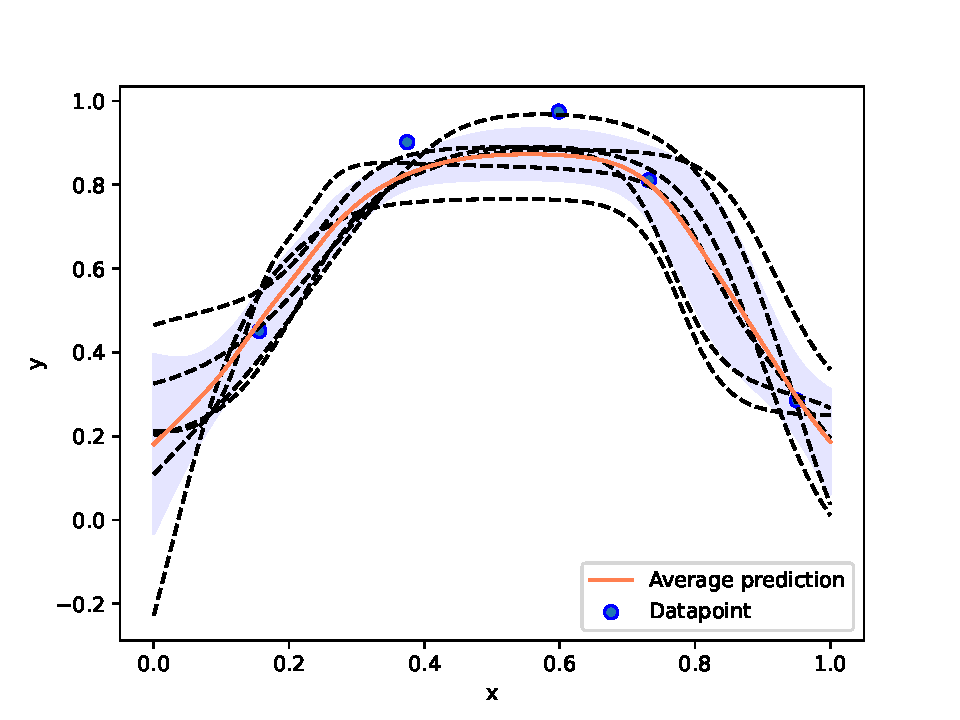
\includegraphics[width=\textwidth,height=\textheight,keepaspectratio]{pics/figure_simple_BNN.pdf}
    \caption{Sampled neural networks from a predictive posterior that is based on a Gaussian prior and a Gaussian likelihood on the 6 datapoints. The average prediction of the networks are plotted along with a filled area defined by the average plus minus the standard deviation of the network predictions to represent uncertainty.}
    \label{fig:simple_BNN}
\end{figure}

\noindent
A simple example, inspired by \cite{neal2012bayesian}, will illustrate the general concept of Bayesian learning for neural networks and the inefficiency of brute force methods. Figure \ref{fig:simple_BNN} shows 6 BNNs whose weights and biases were drawn from independent standard normal prior distributions except output weights, which had a standard deviation of $\frac{1}{\sqrt{16}}$. The networks performs regression on 6 datapoints for which the prior and the likelihood was based. \\
\\
The 6 networks was chosen from a larger pool of $10^5$ networks whose weights and biases were sampled from identical prior distributions. The likelihood was computed for each of these networks and scaled so that the largest likelihood was 1. The networks were then accepted with the probability of this scaled likelihood for which only 6 was accepted. This approach resembles rejection sampling and embodies the posterior in \ref{eq:posterior} by making the prior control the generation of candidate networks and the likelihood control which of these candidates are rejected.\\
\\
We follow the suggestion of \cite{neal2012bayesian} to model regression tasks with a conditional distribution for the real valued targets $\boldsymbol{y}_k$, from $k$ neural networks with outputs $f_k(\boldsymbol{x})$, defined by a Gaussian 
\begin{equation}\label{eq:regr_taget_distribution}
    p(\boldsymbol{y} \mid \boldsymbol{x}) = \prod_k \frac{1}{\sqrt{2 \pi} \sigma_k} \exp{- \frac{\lr{f_k(\boldsymbol{x}) - y_k}^2}{2 \sigma_k^2}}
\end{equation}
with mean $f_k(x)$ and standard deviation $\sigma_k$ as a hyperparameter, which we chose to be $\sigma_k = 0.1$ for all $k$.
\\
\\
The optimal way to predict the target associated with various new examples, assuming we want to minimize the expected squared error, is to predict the mean of the predictive distribution in equation \ref{eq:post_pred_distribution}. For a regression model defined by equation \ref{eq:regr_taget_distribution} this is equal to predicting 
\begin{equation*}
    \hat{\boldsymbol{y}}^{(n+1)} = \int f\lr{\boldsymbol{x}^{(n+1)}, \boldsymbol{\theta}} p\lr{\boldsymbol{\theta} \mid \lr{\boldsymbol{x}^{(1)}, \boldsymbol{y}^{(1)}}, \dots, \lr{\boldsymbol{x}^{(n+1)}, \boldsymbol{y}^{(n+1)}}} \, d \boldsymbol{\theta}
\end{equation*}
As we can only sample from this distribution we resort to a Monte Carlo approximation by averaging over the 6 functions drawn from the posterior as in equation \ref{eq:empirical_mean_MC}. This is also equivalent to minimizing mean squared error. The average is shown in \ref{fig:simple_BNN} by the dotted line. But Bayesian inference can do more than a single-valued guess. By examining the function we can also see the uncertainty of the guesses, for example how rapidly uncertainty increases beyond the region of the datapoints. 
\\
\\
\textcolor{red}{Add text on how we don't need to regularize, and make a train/test split and other perks of BNNs that Neal mentions (perhaps just refer to him instead of showing/arguing for them. MacKay1991 mentions that BNN applies Occams Razor automatically.}\\
\\
This shows some of the perks of using Bayesian inference for neural networks, but what remains is the downside of computational time. Generating $10^5$ samples to get 6 draws from the posterior not very efficient and this only becomes more infeasible as the number of datapoints increase. In section \ref{sec:MCMC} we discuss how to sample more effectively from the posterior using Markov-Chain Monte Carlo methods and in \ref{sec:ADVI} we introduce the approach of variations inference for approximating intractable integrals. Another unresolved matter is how to choose the prior, and how this choice affects our results. This is discussed in \ref{sec:priors} while how to efficiently choose the parameters of the prior is discussed in \ref{sec:hier_models}.


\section{Priors}\label{sec:priors}
From section \ref{sec:bayesian_stat} and the example given in section \ref{sec:simple_BNN} it is seen that Bayesian inference starts with a prior for the model parameters, which is suppose to embody ones prior beliefs about the assigned task. However in neural networks the relationship between parameters and the problem can be very abstract and not as intuitive as in other machine learning models like linear regression models or SVMs. \\
\\
\cite{neal2012bayesian} stresses that even though it can seem like BNNs can be threatened by a lack of a suitable prior this is not the case, as much past work shows useful criteria for selecting suitable priors, even without full understanding of what the prior over the parameters will mean in terms of the output of the network. \cite{mackay1991} and \cite{MacKay1992} has produced results, that Neal describes as at least reasonable, by giving the parameters Gaussian prior distributions. He lets the variance of these distribution be selected as a hyperparameter, which allows the model to adapt to the data. We must state however, that we do not suggest that this is the correct prior to use, as each learning problem is unique. In his work MacKay emhasizes the advantage of hierachichal models described in section \ref{sec:hier_models}.\\
\\
In a BNN the role of the hyperparameters for the priors of the parameters correspond roughly to he role of the weight decay constant $\alpha$ in equation \ref{eq:reg_obj_func} used in training of a conventional neural network. But as noted by \cite{neal2012bayesian} these hyperparameters in BNNs can be found without the need for a validation set.



\section{Hierarchical Models} \label{sec:hier_models}
\textcolor{red}{TÆNKER VI KAN SKRIVE LIDT OM HIERAKISKE MODELLER OGSÅ - KAN EVENTUELT FLYTTES ANDET STEDS HEN HVIS DET PASSER BEDRE.}

\clearpage
\section{Markov chain Monte Carlo}\label{sec:MCMC}
 As we mentioned in section \ref{sec:bayesian_stat} the posterior distribution is often intractable and therefore not possible to derive any analytical solution of it. Therefor we need simulation based methods. We want to be able to calculate posterior summaries like $\mathbb{E}_p\left[f(\boldsymbol{\theta})\right]$ where $f(\boldsymbol{\theta})$ is our model and the expectation is taking under the posterior distribution. Such an expectation is straight forward to approximate when dealing with nice and low dimensional distributions, with simple Monte Carlo methods as described in section \ref{sec:MC_methods}. Other Methods like importance sampling has often been proposed in the litterateur for simple problems, but rarely for high-dimensional problems as we face with Neural Networks.
 \\
 \\
 For more complex models, these methods are not at all useful in practise, a more relevant collection of methods, are the
 Markov chain Monte Carlo (MCMC) methods. The main idea is to simulate a Markov chain, which has the posterior distribution as it's stationary distribution. As a discussion of the different MCMC methods would be rather hard to understand without the fundamental knowledge of Markov chains, we will summarize the most important concepts in the next section. The curious reader is encouraged to see \cite{lawler2006introduction} for a deeper discussion of this subject.
 
\subsection{Definition and Basic Results for Markov chains}
First we define a stochastic process, which is a set of random variables that are defined over some probability space $\left\{X^{(t)} \right\}_{t\in T}$, where $T\subset \mathbb{R}$ is the indexation and may be considered as a temporal or a time index. In the context of Machine Learning, the set $T$ can be interpreted as the iterations of a simulation scheme. In stochastic simulation we typically have that $T=\mathbb{N}$ and we can write the stochastic process as $\left\{X^{(n)}\right\}_{n\geq 0}$, where $n$ reminds us that we have discrete index set. Throughout this thesis we will only consider discrete time stochastic processes, since this is most relevant when discussing stochastic simulation. \\
The set $\mathbb{S}$ is the space of the process $\left\{X^{(n)} \right\}_{n\geq 0}$, and denoted the state space. The state space can be any mathematical set, but in most applications it is the set of integers $\mathbb{N}$ or numbers on the real line $\mathbb{R}$.\\
\\
In Bayesian modelling we consider the model parameters $\boldsymbol{\theta}$ as a random variable and therefor, we can consider a sequence of generated model parameters as a stochastic process. In this section we introduce the basic theory, and we will let $\{\boldsymbol{\theta}^{(n)}\}_{n\geq 0}$ denote the stochastic process of interest.\\ \\
The objective with the BNN model is as early mentioned to make predictions for some unknown test cases. For this we either need the posterior predictive distribution from equation \ref{eq:post_pred_distribution} which is often not possible to derive analytically or we might be interested in an expectation of a model with respect to the posterior distribution.
We call the distribution we wish to sample from the target distribution and denote it $\hat{p}(\cdot)$. The target distribution in Bayesian statistics in often the posterior and thus $\hat{p}(\boldsymbol{\theta})\equiv p(\boldsymbol{\theta}\mid \mathbf{X},\mathbf{y})$. Let us now assume we want to calculate an expectation of some function $\alpha(\boldsymbol{\theta})\equiv f_i(\mathbf{x}^{(n+1)};\boldsymbol{\theta})$ with respect to the target distribution, that is
\begin{equation}\label{eq: expectation_under_posterior}
    \mathbb{E}\left[\alpha(\boldsymbol{\theta})\right]=\int \alpha(\boldsymbol{\theta})\hat{p}(\boldsymbol{\theta}) d\boldsymbol{\theta}
\end{equation}
In section \ref{sec:MC_methods} we saw that such an expectation can be approximated by the empirical average, where we have drawn $\boldsymbol{\theta}$ from the target distribution $\hat{p}(\boldsymbol{\theta})$. The draws in simple Monte carlo methods are i.i.d, which is a very inefficient way of drawing samples when the target distribution is complex, often this is not even a possibility.\\
\\
Another way is generate a sequence of dependent variables $\boldsymbol{\theta}^{(n)}$, such a sequence is often generated by simulating a stochastic process $\{\boldsymbol{\theta}^{(n)}\}_{n\geq 0}$ and not an arbitrary stochastic process, but a process that satisfies the Markov property. The Markov property states that to make predictions about a future state of the system, it suffices to consider only the present state of the system and not all the past states. Such a process is called a Markov chain, named after the famous mathematician Andrey Markov. Formally we can write this as $ \boldsymbol{\theta}^{n} \independent (\boldsymbol{\theta}^0,\boldsymbol{\theta}^1, \ldots, \boldsymbol{\theta}^{n-2}) \mid \boldsymbol{\theta}^{n-1}$. The Markov chain is defined by an initial distribution for the first state of the chain $\boldsymbol{\theta}^{(0)}$, and transition probability/density for the next states in the system. We write the transition probability from transitioning from state $\boldsymbol{\theta}$ to another state $\boldsymbol{\theta}^\prime$ as $T(\boldsymbol{\theta}^\prime\mid \boldsymbol{\theta})$. \\
\\
When drawing samples from the stochastic process $\{\boldsymbol{\theta}^{(n)}\}_{n\geq 0}$ we want to make sure that draws are actually coming from the desired distribution $\hat{p}(\boldsymbol{\theta})$ no matter the initial probability. To do this we need the fact that if a Markov chain has a stationary distribution $\pi(\boldsymbol{\theta})$, and reach a state of the chain where this distribution is established the distribution persists. That is if $\boldsymbol{\theta}^{(n)}$ has $\hat{p}(\boldsymbol{\theta})$ as it's distribution, then  $\boldsymbol{\theta}^{(n^\prime)}$ will have the same distribution, and this will hold for all $n^\prime\geq n$. Formally we call this property, the invariance property,
\begin{equation*}
    \pi(\boldsymbol{\theta}^\prime)=\int T(\boldsymbol{\theta}^\prime\mid \boldsymbol{\theta}) \pi(\boldsymbol{\theta})d\boldsymbol{\theta}
\end{equation*}
A sufficient, but not necessary condition that ensures that a particular $\hat{p}(\boldsymbol{\theta})$ is the desired stationary distribution is the detailed balance condition. The condition states if we let $T(\cdot,\cdot)$ be a transition probability which satisfies the following condition $\hat{p}(\boldsymbol{\theta})T(\boldsymbol{\theta}, \boldsymbol{\theta}^\prime) = \hat{p}(\boldsymbol{\theta}^\prime)T(\boldsymbol{\theta}^\prime, \boldsymbol{\theta})$, then $\hat{p}(\cdot)$ is a stationary distribution of the Markov chain associated with the transition probability $T(\cdot,\cdot)$. The detailed balanced condition is proved below, 
\begin{proof}
Suppose that a distribution $\hat{p}(\cdot)$ satisfies the condition of the detailed balance theorem. Then
 \begin{equation*}
     \begin{split}
         &\hat{p}(\boldsymbol{\theta})T(\boldsymbol{\theta},\boldsymbol{\theta}^\prime)= \hat{p}(\boldsymbol{\theta}^\prime)T(\boldsymbol{\theta}^\prime,\boldsymbol{\theta}) \Leftrightarrow \\
          &\int\hat{p}(\boldsymbol{\theta})T(\boldsymbol{\theta},\boldsymbol{\theta}^\prime)d\boldsymbol{\theta}=\int \hat{p}(\boldsymbol{\theta}^\prime)T(\boldsymbol{\theta}^\prime,\boldsymbol{\theta}) d\boldsymbol{\theta} \\
         &= \hat{p}(\boldsymbol{\theta}^\prime)\int T(\boldsymbol{\theta}^\prime,\boldsymbol{\theta})d\boldsymbol{\theta} =\hat{p}(\boldsymbol{\theta}^\prime)
     \end{split}
\end{equation*}
where we have used that $\int T(\boldsymbol{\theta}^\prime,\boldsymbol{\theta})d\boldsymbol{\theta}=1$ since the probability of transitioning from state $\boldsymbol{\theta}^\prime$ to any possible state $\boldsymbol{\theta}\in\mathbb{S}$ must be equal to one. 
\end{proof}
A Markov chain there is ergodic has a unique stationary distribution from which it converges to from any initial state (see e.g \cite{turkman2019computational}). For a Markov chain to be ergodic, we need two conditions for the states of the system and the transition probabilities. These conditions are known as irreducibility and aperiodicity. If we can create an ergodic Markov chain, with transition probabilites satifying the detailed balance condition, we can approximate expectations like the one in equation \ref{eq: expectation_under_posterior} with an empirical average like in equation \ref{eq:empirical_mean_MC},
\begin{equation*}
    \mathbb{E}\left[a(\boldsymbol{\theta})\right]\approx \frac{1}{n}\sum_{i=0}^n a(\boldsymbol{\theta}^{(i)})
\end{equation*}
where $\boldsymbol{\theta}^{(0)},\ldots \boldsymbol{\theta}^{(n)}$ being the states of the chain. Often we discard or burn some of the initial states, since these may not be representative of the desired distribution since the chain has not reached the stationary distribution yet, such a procedure is called burning in the Markov chain. When the chain has reached the stationary distriubtion, it is possible to draw as many identical distributed samples as we wish for, but one should note that any successive samples will be highly correlated with each other and thus not necessarily a good representative for the target distribution. \cite{Goodfellow-et-al-2016} suggest a way to come around this problem, by only returning every n successive sample. Because of both the burning in phase and the time required for the chain to return uncorrelated samples, MCMC is often computational expensive. \\
\\
In order to produce truly independent samples, \cite{Goodfellow-et-al-2016} suggest to run multiple Markov chains in parallel and explains that practitioners often uses a number of chains that are run in parallel, similar to the number of examples in a minibatch and then draw the samples needed from this set of Markov chains. \\
\\
In the next section we will cover a very useful way of generating a Markov chain that converges to the target distribution. 


\subsection{The Metropolis algorithm} \label{sec:Metropolis_Hastings}
The Metropolis algorithm is a Markov chain Monte Carlo (MCMC) method, which is used to sample from a Bayesian posterior. 
The Metropolis (MH) algorithm was originally introduced by \cite{Metropolis1953} and was developed to simulate the states for a system of idealized molecules (\cite{neal2012mcmc}). This was later further developed by \cite{hastings70}, so that the algorithm could now simulate from a general distribution and not just a symmetric one, as it was previously based on. Due to its versatility and simplicity, the Metropolis algorithm is one of the most widely used in MCMC methods.\\
\\
The Metropolis algorithm generates a sequence of stochastic variables by sampling from a probability distribution, more specific the samples are drawn from a proposal distribution, that specifies the probability of moving to a new point in the sample space. \\
As mentioned in section \ref{sec:MCMC}, the main idea is to create a Markov chain that will converge towards a given distribution, so that the target distribution becomes the Markov chain's stationary distribution.  \\
\\
The simple Metropolis algorithm introduced in the original paper by \cite{Metropolis1953} consider a target distribution $\hat{p}(\boldsymbol{\theta})$ and a proposal distribution $q(\boldsymbol{\theta})$. The algorithm generates a Markov chain, by starting the chain at some arbitrarily point generated from the proposal distribution $\boldsymbol{\theta}^{0}\sim q(\boldsymbol{\theta})$ and then proposing a candidate state for the next state in the chain $\boldsymbol{\theta}^{(cand)}$, where this candidate state is drawn from the conditional distribution on the previous state $\boldsymbol{\theta}^{(cand)}\sim q(\boldsymbol{\theta}^{(n+1)}\mid\boldsymbol{\theta}^{(n)})$, and then we decide whether or not to reject this new state based on the relative probability density to the old state. If the relative density is larger than one, we accept the new state, if the relative density is less than one, we accept the new state with probability $\frac{p(\boldsymbol{\theta}^{cand})}{p(\boldsymbol{\theta}^{(n)})}$. The algorithm is written in pseudo code in algorithm \ref{algo_2}.
% Metropolis Algorithm
\begin{algorithm}[h!]\label{algo_2}

\SetAlgoLined
initialize $\boldsymbol{\theta}^0\sim q(\boldsymbol{\theta})$;

\For{$i=1,2,\ldots$}{
Propose: $\boldsymbol{\theta}^{c a n d} \sim q\left(\boldsymbol{\theta}^{(i)} \mid \boldsymbol{\theta}^{(i-1)}\right)$

Acceptance Probability:

$ \alpha\left(\boldsymbol{\theta}^{c a n d} \mid \boldsymbol{\theta}^{(i-1)}\right)=\min \left\{1, \frac{p\left(\boldsymbol{\theta}^{c a n d}\right)}{ p\left(\boldsymbol{\theta}^{(i-1)}\right)}\right\} $

$u \sim  \text { Uniform }(0,1)
$

  \uIf{$u<\alpha$}{
    Accept the proposal: $\boldsymbol{\theta}^{(i)} \leftarrow \boldsymbol{\theta}^{c a n d}$\;
  }
  \Else{
    Reject the proposal: $\boldsymbol{\theta}^{(i)} \leftarrow \boldsymbol{\theta}^{(i-1)}$ \;
  }
    }
\caption{Metropolis algorithm}
\end{algorithm}\\
In the original algorithm the proposal distribution must satisfy the symmetry condition,
\begin{equation*}
    q(\boldsymbol{\theta'}\mid \boldsymbol{\theta})=q(\boldsymbol{\theta}\mid \boldsymbol{\theta'})
\end{equation*}
To show that this works out, and we are in fact sampling from the target distribution, we must show that these transitions from one state to another in the Markov chain leaves the target distribution invariant. For $\boldsymbol{\theta'}\neq \boldsymbol{\theta}$ the algorithm leads to the following transitions densities,
\begin{equation*}
    T\left(\boldsymbol{\theta}' \mid \boldsymbol{\theta}\right)=q\left(\boldsymbol{\theta}' \mid \boldsymbol{\theta}\right) \min \left(1, p\left(\boldsymbol{\theta}'\right) / \hat{p}(\boldsymbol{\theta})\right)
\end{equation*}
The detailed balance condition is thus verified by,
\begin{equation*}
\begin{aligned}
T\left(\boldsymbol{\theta}' \mid \boldsymbol{\theta}\right) \hat{p}(\boldsymbol{\theta}) &=q\left(\boldsymbol{\theta}' \mid \boldsymbol{\theta}\right) \min \left(1, p\left(\boldsymbol{\theta}'\right) / \hat{p}(\boldsymbol{\theta})\right) \hat{p}(\boldsymbol{\theta}) \\
&=q\left(\boldsymbol{\theta}' \mid \boldsymbol{\theta}\right) \min \left(\hat{p}(\boldsymbol{\theta}), \hat{p}\left(\boldsymbol{\theta}'\right)\right) \\
&=q\left(\boldsymbol{\theta} \mid \boldsymbol{\theta}'\right) \min \left(\hat{p}\left(\boldsymbol{\theta}'\right), \hat{p}(\boldsymbol{\theta})\right) \\
&=q\left(\boldsymbol{\theta} \mid \boldsymbol{\theta}'\right) \min \left(1, \hat{p}(\boldsymbol{\theta}) / \hat{p}\left(\boldsymbol{\theta}'\right)\right) \hat{p}\left(\boldsymbol{\theta}'\right) \\
&=T\left(\boldsymbol{\theta} \mid \boldsymbol{\theta}'\right) \hat{p}\left(\boldsymbol{\theta}'\right)
\end{aligned}
\end{equation*}
the transitions proposed by the algorithm thus leaves the target distribution $\hat{p}(\boldsymbol{\theta})$ invariant and thus samples produced by this Markov chain all has the same stationary distribution $\hat{p}(\boldsymbol{\theta})$. One problem arises since the algorithm needs to calculate the relative density of $\frac{p(\boldsymbol{\theta'})}{p\left(\boldsymbol{\theta}\right)}$, but our target distribution is often intractable and thus a analytical solution is not possible. But since the algorithm only need the target distribution for calculating the relative density, we can use that we know that the posterior is equal to the likelihood times the prior up to some constant of normalization and thus we can use this instead of the target distribution directly.\\
\\
The Metropolis algorithm has been used in many application within Bayesian Statistics and often with good results. One major disadvantage with the algorithm is that it produces highly correlated samples as we discussed about MCMC methods in general in section \ref{sec:MCMC}. One way to cope with this problem is to throw away some of the samples or run multiple chains in parallel.\\
\\
A very common feature of the algorithm is the random-walk behavior (\cite{gelmanbda04}). The simulations generated by the Markov chain is often zigging and zagging through the target distribution in a very inefficient way. This can be seen very clearly in figure \ref{fig:MH_sampling}, where 500 samples from the Metropolis algorithm has been generated for a bivariate target distribution with mean $\boldsymbol{\mu}=\left[\begin{array}{l}
0, 
0
\end{array}\right]^\top$ and covariance matrix
$\boldsymbol{\Sigma}=\left[\begin{array}{cc}
1 & 0.6\\
0.6 & 1
\end{array}\right]$\footnote{The python code can be found in appendix \ref{app:MH_code}}. \\
\\
A more generalized version of the algorithm is the one introduced by \cite{hastings70}, which allows for non-symmetric proposal distributions, that is $q(\boldsymbol{\theta}^\prime\mid \boldsymbol{\theta}) \neq q(\boldsymbol{\theta}\mid \boldsymbol{\theta}^\prime)$. To correct for this asymmetry in the proposal distribution, the acceptance ratio is replaced by
\begin{equation}\label{eq: hasti_pasti}
\alpha\left(\boldsymbol{\theta}^{c a n d} \mid \boldsymbol{\theta}^{(i-1)}\right)=\min \left\{1, \frac{q\left(\boldsymbol{\theta}^{(i-1)} \mid \boldsymbol{\theta}^{c a n d}\right) \hat{p}\left(\boldsymbol{\theta}^{c a n d}\right)}{q\left(\boldsymbol{\theta}^{c a n d} \mid \boldsymbol{\theta}^{(i-1)}\right) \hat{p}\left(\boldsymbol{\theta}^{(i-1)}\right)}\right\} 
\end{equation}
One should note that the Metropolis algorithm is an instance of the generalized version, since equation \ref{eq: hasti_pasti} is identical to the acceptance ratio in the original algorithm when allowance for a symmetric distribution. \\
\\
The introduction of an asymmetric proposal distribution, is often useful when we want to increase the speed of the random walk generated by Metropolis algorithm, but this is often not sufficient for complicated models with high-dimensional target distributions as we face with Bayesian Neural Networks (\cite{gelmanbda04}). We will in the next chapter concentrate on a more efficient way of simulating the chain.
\begin{figure}
    \centering
    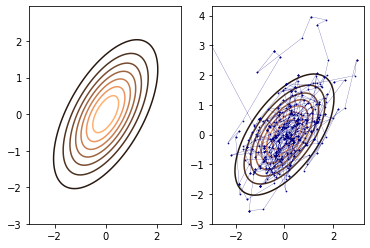
\includegraphics{pics/mh_randomWalk_behavior.png}
    \caption{500 samples generated with the Metropolis Hasting algorithm. The target distribution is a bivariate normal distribution. \textcolor{red}{Make similar y-axis}}
    \label{fig:MH_sampling}
\end{figure}
\clearpage
\section{Hamiltonian Monte Carlo}
As we mention in section \ref{sec:Metropolis_Hastings}, a significant inefficiency in the Metropolis algorithm, is that it often behaves like a random walk and thus the simulations take a longer road while moving through the target distribution, which gives rise to slow simulation. This is espacially a problem when concerning high-dimensional problems, such as Bayesian Neural Networks (\cite{neal2012bayesian}).
Another way to generate proposals with a higher efficiency, is in which the network weights are updated dynamically by simulating Hamiltonian dynamics and then use the Metropolis algorithm to accept or reject these proposals.This algorithm suppress the local random walk behavior and thus allowing it to move much faster and more rapidly through the distribution. The method presented is called Hamilton Monte Carlo (HMC), and is commonly used in computational physics and statistics. The algorithm was originally proposed by \cite{Duane1987216} for calculations used in lattice quantum chromodynamics, but was later introduced to the world of statistics when it was used for Bayesian Neural Networks n \cite{neal2012bayesian}\\
\\
The HMC algorithm reduces correlation between successive sampled states, compared to the Metropolis Hastings algorithm in section \ref{sec:Metropolis_Hastings}, by proposing moves to distant states which maintain a high probability of acceptance due to the approximate energy conserving properties of the simulated Hamiltonian dynamic when using a symplectic integrator\footnote{In mathematics, a symplectic integrator is a numerical integration scheme for Hamiltonian systems.}. The reduced correlation means fewer Markov chain samples are needed to approximate integrals with respect to the target probability distribution for a given Monte Carlo error. For the HMC algorithm we need to construct a differential equation system, that is known to keep the target distribution invariant. If we can achieve this, we can simulate transitions following the solution to this differential equation system and these transitions can be shown to leave the target distribution invariant. Such a differential equations system is often the Hamiltonian dynamics named after William Rowan Hamilton and will be introduced in the next section. 

\subsection{Hamiltonian dynamics}
Before we move to the actual HMC algorithm, we need to become familiar with the concept of Hamiltonian dynamics. Hamiltonian dynamics are used to describe how an object move around in a system. The Hamiltonian dynamics is define by the objects location $\boldsymbol{\theta}\in \mathbb{R}^d$ and it's momentum $\boldsymbol{\rho}\in \mathbb{R}^d$, which in the physics are equivalent to an object's mass times it's velocity at some point in time $t$. The object's location is associated with a potential energy $U(\boldsymbol{\theta})$ and likewise the momentum is associated with a kinetic energy $K(\boldsymbol{\rho})$. The sum of the potential and kinetic energy is regarded as the total energy of the system and often called the Hamiltonian,
\begin{equation*}
H(\boldsymbol{\theta},\boldsymbol{\rho})=U(\boldsymbol{\theta})+K(\boldsymbol{\rho})    
\end{equation*}       
one important feature of the Hamiltonian is that it is constant over time. Taking the partial derivative with respect to time of the location and momentum, shows us how they evolve over time,
\begin{equation}\label{eq:hamilton_equations}
\begin{split}
\frac{d \theta_{i}}{d t}=\frac{\partial H}{\partial \rho_{i}}=\frac{\partial K(,\boldsymbol{\rho})}{\partial \rho_{i}} \\
\frac{d \rho_{i}}{d t}=-\frac{\partial H}{\partial \theta_{i}}=-\frac{\partial U(,\boldsymbol{\theta})}{\partial \theta_{i}}
\end{split}
\end{equation}
where $i=1,2, \ldots,d$. These are named Hamiltonian equations and represents differential equations system. The Hamiltonian equations are very useful, since if we are able to evaluate the partial derivatives from equation \ref{eq:hamilton_equations}, we are able to predict the location and momentum variable of the object at any point in the future $t^\prime>t$.
\subsection{Properties of the Hamiltonian Dynamics}
The Hamiltonian dynamics have several properties, which are very crucial when used in relation to MCMC simulations.\\
\\
\textit{Property of time reversibility:}\\
This property is very important for showing that the HMC transitions, generated by the dynamics, leave the target distribution invariant, since the reversibility of the chain transitions requires reversibility of the dynamics. \\
\\
\textit{Property of conservation:}\\
Secondly we have the property of conservation, that is the dynamics keeps the Hamiltionian invariant. This can easily be verified from equation \ref{eq:hamilton_equations}
\begin{equation}\label{eq:Hamilton_conservation}
    \frac{d \H}{d t}=\sum_{i=1}^{d}\left[\frac{d \theta_{i}}{d t} \frac{\partial \H}{\partial \theta_{i}}+\frac{d \rho_{i}}{d t} \frac{\partial \H}{\partial \rho_{i}}\right]=\sum_{i=1}^{d}\left[\frac{\partial \H}{\partial \rho_{i}} \frac{\partial \H}{\partial \theta_{i}}-\frac{\partial \H}{\partial \theta_{i}} \frac{\partial \H}{\partial \rho_{i}}\right]=0
\end{equation}
In the HMC method, we will use Metropolis updates, with proposals found by the Hamiltonian dynamic. We have that the acceptance probability is one if $\H$ is kept invariant (see e.g \cite{neal2012mcmc}). This is however not possible in practise, and we are only able to keep $\H$ approximately invariant, but we will come back to this issue later. \\
\\
\textit{Property of volume preservation:}
The last crucial property of the Hamiltonian dynamics is the volume preservation property, which gives us that the dynamics preserves volume in the $(q,p)$ space.

\begin{equation*}
    \sum_{i=1}^{d}\left[\frac{\partial}{\partial \theta_{i}} \frac{d \theta_{i}}{d t}+\frac{\partial}{\partial \rho_{i}} \frac{d \rho_{i}}{d t}\right]=\sum_{i=1}^{d}\left[\frac{\partial}{\partial \theta_{i}} \frac{\partial \H}{\partial \rho_{i}}-\frac{\partial}{\partial \rho_{i}} \frac{\partial \H}{\partial \theta_{i}}\right]=\sum_{i=1}^{d}\left[\frac{\partial^{2} \H}{\partial \theta_{i} \partial \rho_{i}}-\frac{\partial^{2} \H}{\partial \rho_{i} \partial \theta_{i}}\right]=0
\end{equation*}

\subsection{Discretizing Hamiltonian Equations}
The Hamiltonian equations describe how an objective evolve in time, which is regarded as a continous variable, but for simulating dynamics on a computer system, we have to approximate the differential equations numerically in some way, by discretizing time. We do this by splitting the time interval $dt$ into small intervals $\epsilon$. We will now present to common ways of handling this. The first is the Euler's Method and lastly the Leapfrog Method.
\\
\\
\textit{Euler’s Method:}
This is one of the most common methods in computational science for solving a differential equation system. For Hamiltonian equations the Euler methods update the location and momentum variable as follows,

\begin{equation*}
\begin{split}
\rho_{i}(t+\epsilon)=\rho_{i}(t)+\epsilon \frac{d \rho_{i}}{d t}(t)=\rho_{i}(t)-\epsilon \frac{\partial U}{\partial \theta_{i}(t)} \\
\theta_{i}(t+\epsilon)=\theta_{i}(t)+\epsilon \frac{d \theta_{i}}{d t}=\theta_{i}(t)+\epsilon \frac{\partial K}{\partial \rho_{i}(t)}
\end{split}
\end{equation*}
According to \cite{neal2012mcmc} a slightly better result can be obtained by,
\begin{equation*}
\begin{split}
\rho_{i}(t+\varepsilon) &=\rho_{i}(t)-\varepsilon \frac{\partial U}{\partial \theta_{i}}(q(t)) \\
\theta_{i}(t+\varepsilon) &=\theta_{i}(t)+\varepsilon \frac{\rho_{i}(t+\varepsilon)}{m_{i}}
\end{split}
\end{equation*}
\textit{Leapfrog method:}\\
Another discretizing scheme often used for simulation Hamiltonian equations, is the Leapfrog method. Whereas the Euler’s method takes full steps for updating location and momentum, the leapfrog method takes a half steps to update momentum value,
\begin{equation*}
\begin{split}
\rho_{i}(t+\epsilon / 2)=\rho_{i}(t)-(\epsilon / 2) \frac{\partial U}{\partial \theta_{i}(t)} \\
\theta_{i}(t+\epsilon)=\theta_{i}(t)+\epsilon \frac{\partial K}{\partial \rho_{i}(t+\epsilon / 2)} \\
\rho_{i}(t+\epsilon)=\rho_{i}(t)-(\epsilon / 2) \frac{\partial U}{\partial \theta_{i}(t+\epsilon)}
\end{split}
\end{equation*}
According to \cite{neal2012mcmc} the Leapfrog method, preserves volume exactly, \textcolor{red}{which is good??} and it is also reversible. 

\subsection{Hamiltonian and Probability: Canonical Distributions}
We now have a slightly better understanding understanding of what is a Hamiltonian and how we can simulate it's dynamics by either the Euler method or the Leapfrog method. We now need to connect this with the MCMC theory from the previous sections. In order to perform this connection, we need to relate the target distribution $\hat{p}(\boldsymbol{\theta})$ and the Hamiltonian, such that we can use the Hamiltonian equations to the target distribution. A way of doing this, proposed by \cite{neal2012bayesian}, is use a concept from statistical mechanics known as the canonical (Boltzman) distribution. The probability distribution of $\boldsymbol{\theta}$ under the canonical distribution can be written as
\begin{equation*}
    \hat{p}(\boldsymbol{\theta})\propto \exp(\frac{-U(\boldsymbol{\theta})}{T})
\end{equation*}
where $U(\boldsymbol{\theta})$ again is the potential energy. $T$ is often called the temperature of the system and usually chosen to be equal to one (\cite{neal2012bayesian}).
One should note that any probability distribution that is nowhere zero can be put into this form by letting $E(\boldsymbol{\theta})=-\log \hat{p}(\boldsymbol{\theta})-\log Z$, for any convenient choice of $Z$.  Since the Hamiltonian is an energy function for the joint state of both position and momentum, we need a joint distribution, which is given by
\begin{equation*}
p(\boldsymbol{\theta},\boldsymbol{\rho})\propto \exp(-\H(\boldsymbol{\theta},\boldsymbol{\rho}))   = \exp(-U(\boldsymbol{\theta}))\exp(-K(\boldsymbol{\rho}))=\hat{p}(\boldsymbol{\theta})p(\boldsymbol{\rho})
\end{equation*}
where the last equality hold since we assume independence between $\boldsymbol{\theta}$ and $\boldsymbol{\rho}$. We now have a joint distribution, in terms of the Hamiltonian function, which we know how to simulate. But we are in fact only interested in the location variable $\boldsymbol{\theta}$ and not the momentum variable $\boldsymbol{\rho}$, which we in some way can interpret as a "helper" variable that enable us to simulate the joint distribution. In order to gain marginal sample from the target distribution only, on can simply throw away the samples the momentum distribution, because they are independent anyway. Since we can interpret the momentum variable as a  helper variable, we are allowed freely to decide the marginal distriubtion $p(\boldsymbol{\rho})$. The litterautr often choose it to be gaussian, this $\boldsymbol{\rho}\sim \mathcal{N}\left(0, \Sigma \right)$, where $\Sigma$ is some symmetric, positive-definite mass matrix and often chosen to be diagonal, such that $\boldsymbol{\rho}$ is d-dimensional multivariate normal where the variables are independent. 
The Hamiltonian equations from equation \ref{eq:hamilton_equations} can now be written as,
\begin{equation*}
\begin{split}
\frac{d \theta_{i}}{d t}&=\left[\Sigma^{-1}\rho\right]_i \\
\frac{d \rho_{i}}{d t}&=-\frac{\partial U}{\partial \theta_i}
\end{split}
\end{equation*}





\subsection{Hamiltonian Monte Carlo}
We start the HMC algorithm from an initial state $\boldsymbol{\theta}_0$ $\boldsymbol{\rho}_0$, and then we simulate the Hamiltonian dynamics for $t+\epsilon$ using the Leapfrog method. We choose the Leapfrog method since \cite{betancourt2017conceptual} shows it to be more effective. The states generated for the position and momentum variable at the end of the Leapfrog simulation is used as proposals for a new state $(\boldsymbol{\theta}^\prime,\boldsymbol{\rho}^\prime)$. The proposed stats are accepted according to the Metropolis acceptance criteria,
\begin{equation*}
\begin{split}
    \alpha\left((\boldsymbol{\theta},\boldsymbol{\rho}) \mapsto (\boldsymbol{\theta}^\prime , \boldsymbol{\rho}^\prime )\right) &= \min\left\{1, \frac{p(\boldsymbol{\theta}^\prime,\boldsymbol{\rho}^\prime)}{p(\boldsymbol{\theta},\boldsymbol{\rho})} \right\}\\
    &= \min\{1,\exp\left(\log p(\boldsymbol{\theta}^\prime,\boldsymbol{\rho}^\prime)- \log p(\boldsymbol{\theta}, \boldsymbol{\rho})  \right)\\
    &= \min \left\{1,\exp\left(-\H(\boldsymbol{\theta}^\prime,\boldsymbol{\rho}^\prime) +\H(\boldsymbol{\theta},\boldsymbol{\rho})\right) \right\}
\end{split}
\end{equation*}
If we could simulate the Hamiltonian dynamics exactly, the Metropolis acceptance criteria would always be equal to one, due to the Hamiltonian conservation criteria in equation \ref{eq:Hamilton_conservation} which would give $\min \{1, \exp (0)\}=1$. But since we cannot simulate the Hamilton dynamics exactly and we need to approximate them with the Leapfrog scheme introduced earlier. We can however see that if we choose a proper way of discretize the dynamics, the term  $\H(\boldsymbol{\theta},\boldsymbol{\rho})-\H(\boldsymbol{\theta}^\prime,\boldsymbol{\rho}^\prime)$ in the exponent should be small, thus a high acceptance rate. This is a very clever way of making proposals, since we can make very large and uncorrelated moves in the state space, while keeping a high acceptance of probability. The algorithm is written in pseudo code in algorithm 

\begin{algorithm}[h!]\label{algo_2}

\SetAlgoLined
$\text{Given } \theta^{0}, \epsilon, L, \mathcal{L}, M$:
\For{m=1 to M}{
Sample $r^{0} \sim \mathcal{N}(0, I)$ \\
Set $\theta^{m} \leftarrow \theta^{m-1}, \tilde{\theta} \leftarrow \theta^{m-1}, \tilde{r} \leftarrow r^{0}$
\For{i = 1 to L}{
Set $\tilde{\theta}, \tilde{r} \leftarrow \operatorname{Leapfrog}(\tilde{\theta}, \tilde{r}, \epsilon)$
With probability $\alpha=\min \left\{1, \frac{\exp \left\{\mathcal{L}(\tilde{\theta})-\frac{1}{2} \tilde{r} \cdot \tilde{r}\right\}}{\exp \left\{\mathcal{L}\left(\theta^{m-1}\right)-\frac{1}{2} r^{0} \cdot r^{0}\right\}}\right\}, \text { set } \theta^{m} \leftarrow \tilde{\theta}, r^{m} \leftarrow-\hat{r}$

}
}
\caption{Metropolis algorithm}
\end{algorithm}







\subsection{No-U-Turn Hamiltonian Monte Carlo}
In this section we will talk about an algorithm developed by \cite{hoffman2011nouturn}.


\section{Variational Inference Methods}
In the purpose of approximating a posterior distribution,  Variational inference (VI) is an alternative to MCMC methods, for taking a fully Bayesian approach when we have complex posterior distribution which is difficult to evaluate directly or generate samples from. Whereas MCMC techniques, provide a numerical approximation, VI provides a locally-optimal solution to an approximation of the posterior, thus VI turns approximate posterior inference into an optimization problem (\cite{VI}). We consider a family of approximating densities of the model parameters $q(\boldsymbol{\theta} ; \boldsymbol{\phi})$, parameterized by $\boldsymbol{\phi} \in \boldsymbol{\Phi}$.VI finds the parameters that minimize the KL divergence from equation \ref{eq: KL} to the posterior,
$$
\boldsymbol{\phi}^{*}=\underset{\phi \in \boldsymbol{\Phi}}{\arg \min } \mathrm{KL}(q(\boldsymbol{\theta} ; \boldsymbol{\phi}) \| p(\boldsymbol{\theta} \mid \boldsymbol{x})) .
$$
The optimized $q(\boldsymbol{\theta};\boldsymbol{\phi}^{*})$ is then an approximation of the posterior distribution. This is often not computable, since it requires that we are able to calculate the evidence $\ln p(\boldsymbol{X})$ which we often are not able to. Instead we maxmise the Evidence lower bound (ELBO)
\begin{equation*}
    \mathscr{L}(\boldsymbol{\phi})=\mathbb{E}_{q(\boldsymbol{\theta})}[\log p(\boldsymbol{x}, \boldsymbol{\theta})]-\mathbb{E}_{q(\boldsymbol{\theta})}[\log q(\boldsymbol{\theta} ; \boldsymbol{\phi})]
\end{equation*}
We note that the E


\subsection{Automatic Variational Inference}\label{sec:ADVI}
\subsection{Bayes by Backprop}
\textcolor{red}{Maybe this section should be something we could mention as for future work? as the PYMC VI implementation is build on ADVI (\ref{sec:ADVI}) and not Bayes by Backprop? Otherwise we should check if we can build this our selfs? I have not yet seen it implemented.}

\chapter{Evaluation of Neural Network Models} \label{chap:eval_NN}
This chapter examines the applications of non-Bayesian and Bayesian neural networks using two datasets. First a dataset on housing prices in Boston for regression and secondly a dataset on credit card client defaults for classification. We will evaluate the models by comparing and examining their accuracy as well as computational runtime.
\\
\\
All models are implemented in the programming language Python and the code can be found in the appendix. The specification on the computer that has performed the computation of the models are shown in appendix \ref{app:specs} along with the packages used and their versions.
\\
\\
In section \ref{sec:Boston_housing} we examine the median prices on houses in specific areas of Boston based on a number of features shown in table \ref{tab:Boston_Housing}. We aim to predict unknown median prices based on these features using regression. Section \ref{sec:credit_default} examines defaulting payments on credit card clients in Taiwan. Our objective is in this case to predict the probability of defaults and describe how these can be used for classifying whether a client will default or not.

\section{Predicting House Prices in Boston}\label{sec:Boston_housing}
The Boston housing data was originally introduced by \cite{HARRISON197881}, who investigated the effect of air pollution on house prices.
The dataset contains information collected by the U.S Census Service concerning housing in the area of Boston Massachusetts. The sample contains 506 examples, where each example represents a unique area and has 14 features, which are shown in table \ref{tab:Boston_Housing}. In this section we examine how to use the theory presented in the previous chapters for using non-Bayesian and Bayesian neural networks to predict the median value of owner-occupied homes in thousands.  
\\
\\
The objective is to make good predictions in terms of a low mean squared error (MSE) on unseen data. For this reason we split the data, so that some data are only used as a test set for evaluating the model, while some other data are used as a training set for training the model. We also make another split to generate a validation set, which is used to calculate the loss for each training epoch for determining the stopping time of early stopping, see section \ref{sec:early_stopping}. We perform the same splits for all of the neural networks, so that we ensure that they are trained and tested on the same data, meaning that we also have a validation set for the neural networks not using early stopping. This allows us to use the validation set to illustrate the validation loss and training loss for each epoch to examine possible overfitting in the non-Bayesian neural networks. First we split the data, so that 30\% are used for test data and the remaining for training and validation. This remaining data are then split, so that 70 \% of the remaining data are used only for training and the rest is used for the validation set. To avoid the possibility that the data are sorted in some undesired way we choose to shuffle the data randomly before splitting it. 
\\
\\
 A predictive model for house prices can be very useful in many applications. It could help a real estate developer determine the selling price of newly developed houses or it could help a buyer who wants to buy a house in a certain area. It can also be useful for a property investors to determine the price for an area to invest in.
 


\begin{table}
\caption{Table of features in Boston Housing data. The dataset contains 506 examples each with 14 features. Data can be downloaded on:\\ \href{http://lib.stat.cmu.edu/datasets/boston}{http://lib.stat.cmu.edu/datasets/boston}.}
\label{tab:Boston_Housing}
\centering
\resizebox{\textwidth}{!}{%
\begin{tabular}{|l|l|}
\hline
\multicolumn{1}{|c|}{{\cellcolor{ashgrey}{
 \textbf{Feature name}}}} & \multicolumn{1}{|c|}{{\cellcolor{ashgrey}{
 \textbf{Feature description}}}} \\ \hline
crim              &   Per capita crime rate by town     \\ \hline
zn                &  Proportion of residential land zoned for lots over 25,000 sq. ft                  \\ \hline
indus             &   Proportion of residential land zoned for lots over 25,000 sq. ft                   \\ \hline
chas              & Charles River dummy variable\\
&  (= 1 if tract bounds river; 0 otherwise)   \\ \hline
nox               &  Nitric oxide concentration (parts per 10 million)                    \\ \hline
rm                &   Average number of rooms per dwelling                   \\ \hline
age               &    Proportion of owner-occupied units built prior to 1940                  \\ \hline
dis               &   Weighted distances to five Boston employment centers                   \\ \hline
rad               &   Index of accessibility to radial highways                   \\ \hline
tax               &   Full-value property tax rate per $10,000 $                  \\ \hline
ptratio           &   Pupil-teacher ratio by town                   \\ \hline
b                 & $1000(Bk - 0.63)^2$, where Bk is the proportion of people of   \\ 
& African American descent by town                     \\ \hline
lstat             &    Percentage of lower status of the population                   \\ \hline
medv              &  Median value of owner-occupied homes in $1000s$                    \\ \hline
\end{tabular}}
\end{table}



\subsection{Regression with Neural Networks}\label{sec:regre_w_NN}
We perform regression with the neural networks listed in table \ref{tab:Boston_NN_performance}. All of these are implemented using MSE as loss function, the ReLU function from equation \ref{eq:relu} as activation function on every hidden layer and no activation function for the output layer. All of the networks have 10 neurons in each hidden layer and are trained with 300 epochs using ADAM described in section \ref{sec:ADAM}. We have selected these settings as they were found to provide acceptable results after experimenting with several other options. We reuse these settings for all the neural networks to make them more suitable for comparison. 
\\
\\
The training and validation loss for each training epoch is shown for the networks in figure \ref{fig:Boston_NN_nohidden_wd_loss}, figure \ref{fig:Boston_NN_1hidden_wd_loss} and figure \ref{fig:Boston_NN_1hidden_noreg_loss}. These figures show that the validation loss is almost always lower than our training loss for all of the networks, which might indicate that neither of the models overfit, but might also be due to chance. 
\noindent
We examine a neural network with no hidden layers and weight decay, as this is equal to linear regression with weight decay. We include this to test if a neural network is beneficial compared to the simple approach of using linear regression. We see from table \ref{tab:Boston_NN_performance} that we get a smaller amount of test and train error when using one hidden layer even without regularization, which indicates that using a neural network for this problem is indeed useful.
\\
\\
When we use a neural network with one hidden layer and weight decay we get a slightly smaller test loss and slightly larger train loss, than we did when using one hidden layer and no regularization, indicating that we might have prevented some overfitting by introducing weight decay. 
\\
\\
We also test regularizing the network of one hidden layer by using the method of early stopping, and see that this gives a slightly smaller test loss and larger train loss than the network regularized with weight decay. So early stopping might have prevented overfitting better than weight decay.
Early stopping is, as mentioned in section \ref{sec:early_stopping}, most useful when validation loss begins to increase at some point before ending the training. We see from figure \ref{fig:Boston_NN_1hidden_noreg_loss} that this is not the case, but that the validation loss begins to oscillate slightly more after the stopping epoch. If test loss had the same behavior then this might explain why early stopping attained a smaller test loss than weight decay. We examined training periods with more epochs, to see if validation loss would begin to increase at some later point, but both validation and training error continued to be around the same level as in epoch 300. 
\begin{table}[h!]
\caption{Performance measurement for neural network models on Boston Housing data. Early stopping ran 255 epochs with patience 10 and $\delta_{\text{min}}=0.1$. For weight decay on all networks we select $\alpha = 0.3$ as the regularization constant. The Python code used to implement these neural networks can be seen in appendix \ref{app:Boston_NN}}
\label{tab:Boston_NN_performance}
\resizebox{\textwidth}{!}{%
    \begin{tabular}{|l|l|l|l|}
    \hline
    \multicolumn{1}{|c|}{{\cellcolor{ashgrey}{
     \textbf{Model}}}} & \multicolumn{1}{|c|}{{\cellcolor{ashgrey}{
     \textbf{Train MSE}}}}  &\multicolumn{1}{|c|}{{\cellcolor{ashgrey}{
     \textbf{Test MSE}}}}            & \multicolumn{1}{|c|}{{\cellcolor{ashgrey}{
     \textbf{Runtime (s)}}}}   \\ \hline
     No hidden layers \& weight decay & 81.798 & 60.074  &   10.64           \\ \hline
    1 hidden layer \& no regularization & 36.539 &  25.650  &   10.14           \\ \hline
    1 hidden layers \& weight decay & 37.103 & 25.542  &   10.81         \\ \hline
    1 hidden layers \& early stopping  & 37.512 & 25.223  &  8.66             \\ \hline
    \end{tabular}
}
\end{table}
\begin{figure}[h!]
    \centering
    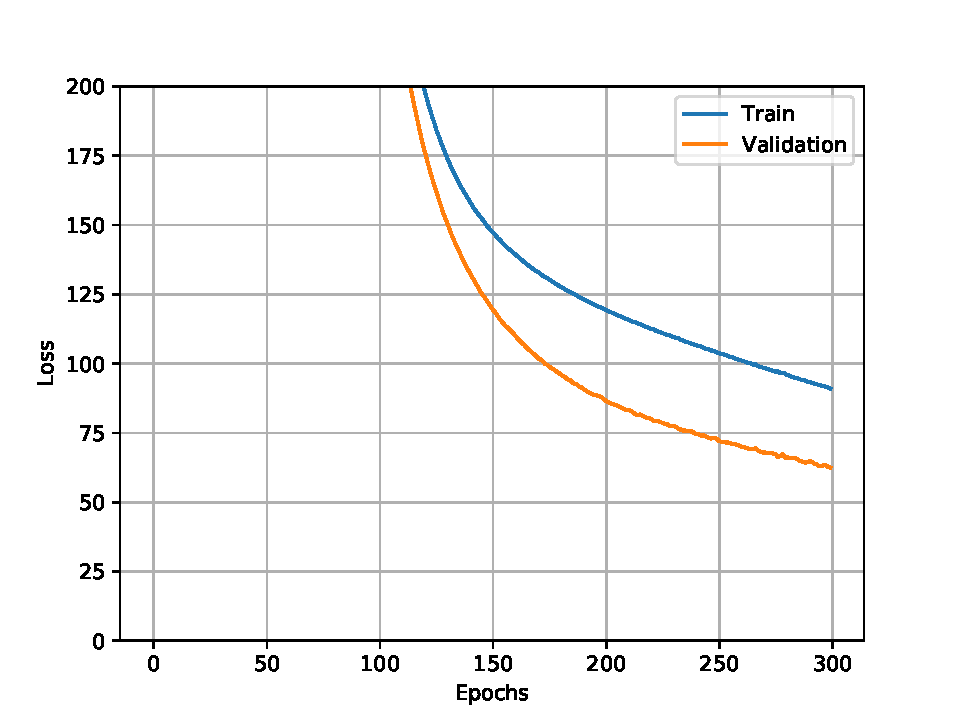
\includegraphics[width=0.95\textwidth]{pics/figure_Boston_NN_nohidden_wd_loss.pdf}
    \caption{Loss on training and validation set during training epochs for the neural network with no hidden layers weight decay.}
    \label{fig:Boston_NN_nohidden_wd_loss}
\end{figure}

\begin{figure}
    \centering
    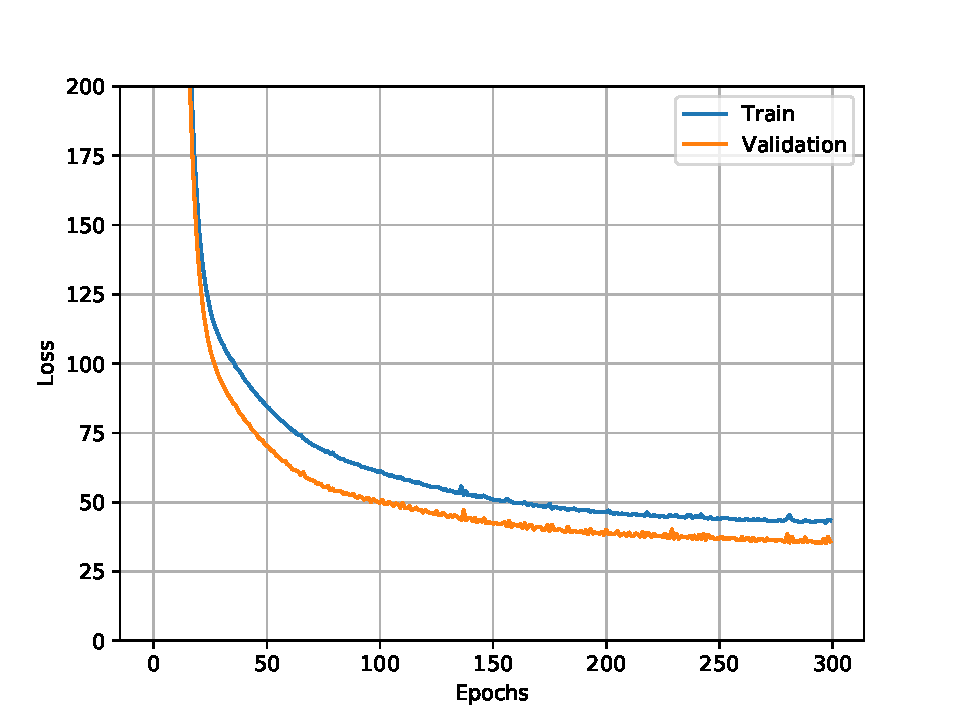
\includegraphics[width=\textwidth]{pics/figure_Boston_NN_1hidden_wd_loss.pdf}
    \caption{Loss on training and validation set during training epochs for the neural network with 1 hidden layers and weight decay. }
    \label{fig:Boston_NN_1hidden_wd_loss}
\end{figure}


\begin{figure}
    \centering
    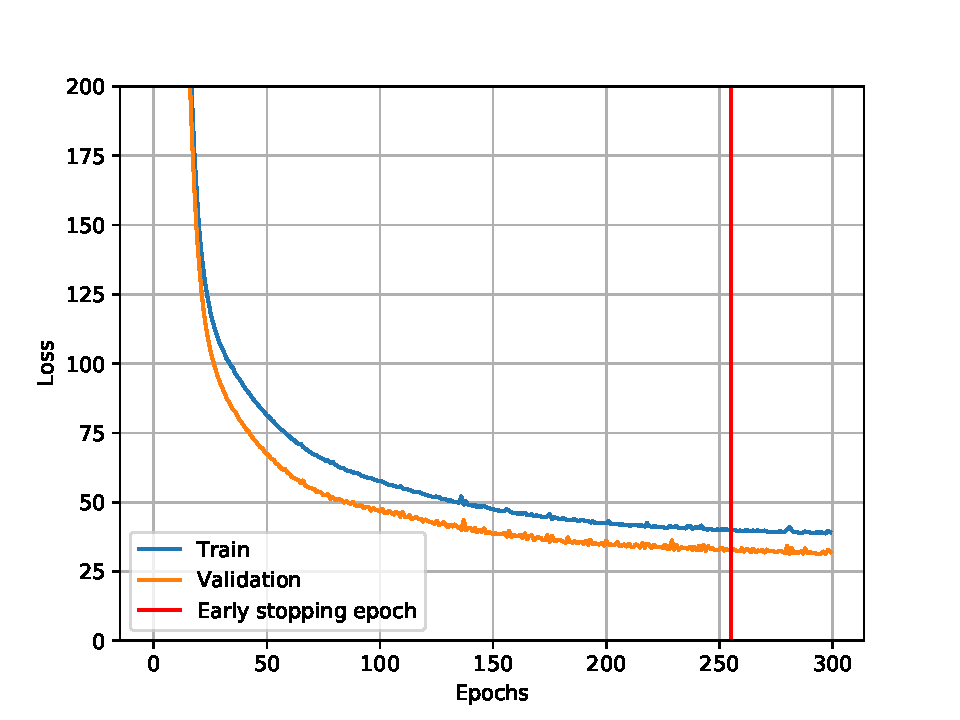
\includegraphics[width=\textwidth]{pics/figure_Boston_NN_1hidden_noreg_loss.pdf}
    \caption{Loss on training and validation set during training epochs for the neural network with one hidden layer \& no regularization. These losses are the same as for the network with 1 hidden layer and early stopping up to the stopping time on epoch 255 indicated by the red vertical line. It can be seen that validation loss is somewhat flattening and decreasing in oscillations around epoch 255, which might be what made the early stopping algorithm indicate no further improvements in validation loss, given the chosen patience of 10 epochs and $\delta_{\text{min}} = 0.1$, and stop the training.}
    \label{fig:Boston_NN_1hidden_noreg_loss}
\end{figure}
\clearpage

\subsection{Regression with Bayesian Neural
Networks}\label{subsec:regression_w_bnn}
We perform regression with the Bayesian neural networks listed in table \ref{tab:Boston_BNN_performance}. All of these networks are implemented with a Gaussian likelihood with mean equal to the network output and standard deviation $\sigma$ equal to 1. We have chosen to run three kinds of BNNs. First a BNN with no hidden layers which corresponds to Bayesian linear regression. Then a BNN with one hidden layer, where we follow the example of \cite{mackay1991} and \cite{MacKay1992} and choose a Gaussian prior on the parameter weights, which we choose more specifically to be $\mathcal{N}(0,0.1)$ . Lastly a hierarchical BNN with one hidden layer, with a $\mathcal{N}(\mu,\sigma)$ prior for the network weights. The parameter $\mu$ is chosen to follow a $\text{Cauchy}(\alpha,\beta)$ distribution and the standard deviation $\sigma$ follows a $\text{Half-Normal}(\nu)$ distribution in order to avoid negative values. The hyper-prior distributions are parametric and therefore require that we specify the hyperparameters for these.
After experimenting with different choices of parameters for the hyper-prior, we choose $\alpha=0$, $\beta=1$ and $\nu=1$. All BNN models have 10 hidden neurons and use ReLU in the hidden layer for ease of comparison, and in order to evaluate on the same models as in section \ref{sec:regre_w_NN} but with a Bayesian approach. \\
\\
We sample from the posterior distribution of the model parameters using the NUTS algorithm examined in section \ref{sec:nuts}.
We sample from three Markov Chains in parallel to get more independent samples, as described in section \ref{sec:MCMC}, where we for each chain draw $3000$ samples from the posterior distribution. A burn-in phase of $1000$ has been chosen for each chain. For the dual averaging algorithm we chose an
acceptance probability $\delta$ of $90\%$ , as it provided us with most acceptable results. All other inputs used for the NUTS algorithm were not chosen by us, as we used the default settings in \texttt{PyMC3}. 
Predictions are made by sampling from the posterior predictive distribution. We generate a total of $3000 \times 3$ samples from the posterior predictive distribution, and to make a single best guess in terms of minimizing MSE we make a prediction by taking the mean of the posterior predictive distribution. 
\\
\\
From table \ref{tab:Boston_BNN_performance} we see that both BNNs with one hidden layer outperform the baseline model with no hidden layers. As a BNN with no hidden layers corresponds to performing Bayesian linear regression, this indicates that using Bayesian inference in a neural network is more useful than using Bayesian inference in a simple linear regression, in this particular case. We also note that all the BNN models are outperforming the non-Bayesian neural networks in terms of MSE both on the training data, but also on the unseen test data. However, it takes about $140$ times longer to run a BNN with one hidden layer than a similar non-Bayesian neural network. So even though the BNNs get a loss-wise better result in this case, it might not be so if one has a time budget lower than the runtime found in table \ref{tab:Boston_BNN_performance}.
\\
\\
However, the computational burden that comes with BNNs also comes with the benefit of producing a distribution for the predictions. This enables us to consider more possible outcomes when making predictions and to have a better idea of the uncertainty in our predictions. The posterior predictive distribution is shown as a histogram in figure \ref{fig:post_pred_noston} for different examples in the test dataset. Such a distribution can be useful in decision making. Consider the example of a property investor, who would like to invest in a certain area. If two areas, according to our model, have the same mean median price he might wish to invest in the area that has the most narrow posterior predictive distribution i.e. lowest standard deviation, so that he is least likely to be surprised by the actual median price. 
\\
\\
We have chosen to use the mean of the posterior predictive distribution for predictions, as this is usually the best measure for central tendency when the distribution is symmetric, but from figure \ref{fig:post_pred_noston} we can see that we might want to take some caution against doing this, as the posterior predictive distribution of the chosen examples show bimodal tendencies and are not symmetric. This shows how to critically evaluate our model when we have access to the distribution of a models predictions. With non-Bayesian neural networks, we only get a single point estimate for the model parameters, and do not factor in the full range of possibilities. Despite these examples we still use the mean for prediction as it provides us with acceptable results. 

\begin{table}
\caption{Performance measurement for Bayesian neural network models on Boston housing data. The Python code used to implement these Bayesian neural networks can be seen in appendix \ref{app:Boston_BNN}.}
\label{tab:Boston_BNN_performance}
\resizebox{\textwidth}{!}{%
\begin{tabular}{|l|l|l|l|}
\hline
\multicolumn{1}{|c|}{{\cellcolor{ashgrey}{
\textbf{Model}}}}   &  \multicolumn{1}{|c|}{{\cellcolor{ashgrey}{
 \textbf{Train MSE}}}} & \multicolumn{1}{|c|}{{\cellcolor{ashgrey}{
 \textbf{Test MSE}}}}           & \multicolumn{1}{|c|}{{\cellcolor{ashgrey}{
 \textbf{Runtime (s)}}}}      \\ \hline
No hidden layers &  28.480 &   17.760    &     211.63      \\ \hline
1 hidden layer    &  11.391  & 9.340        &    1496.69                     \\ \hline
Hierarchical with 1 hidden layer     &      14.135          &  10.869  &  1851.46   \\ \hline
\end{tabular}
}
\end{table}
\begin{figure}
    \centering
    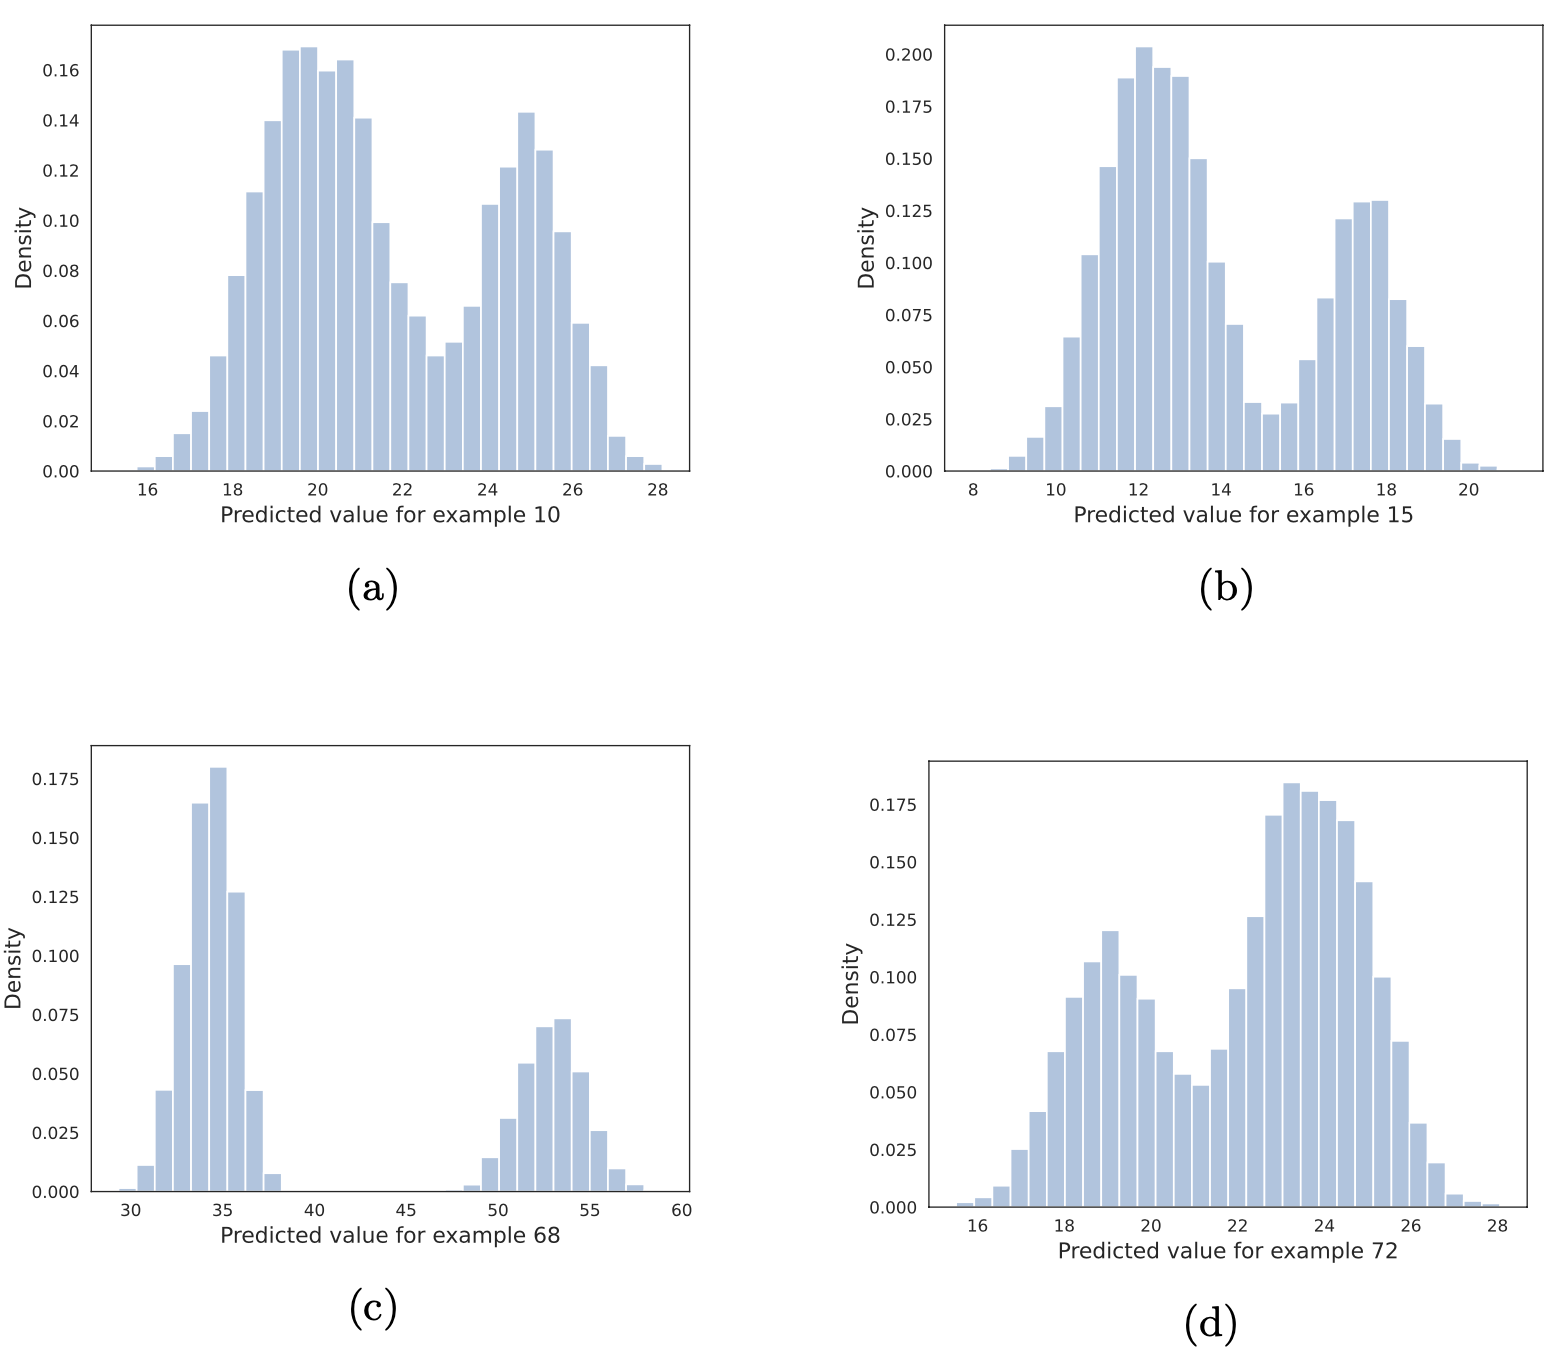
\includegraphics[width=\textwidth]{pics/post_pred_Boston.png}
    \caption{A histogram of predictions generated by samples from from the posterior predictive distribution for example 10, 15, 68 and 72 in the test dataset. The predictions are based on the 1 hidden layer BNN model}
    \label{fig:post_pred_noston}
\end{figure}

\clearpage
\section{Predicting Defaults of Credit Card Clients} \label{sec:credit_default}
The default of credit card clients dataset contains information collected by a Taiwan bank in 2005, on $30.000$ credit card clients. The data contains 25 variables, which are represented in table \ref{tab:credit_card_features}. Due to the computational complexity of the BNN model, we choose to subsample our dataset, such that it only contains $300$ train examples and $100$ test examples. We also perform the same splits of the data as in section \ref{sec:Boston_housing}, meaning that 30 \% of the data are contained in a test set, and the remaining data are afterwards split into 70 \% training data and 30 \% validation data. The data are shuffled before splitting, to prevent that it should be sorted in an undesired way.
\\
\\
The default of credit card clients dataset has earlier been used by \cite{Yeh2009TheCO} for predicting the probability of default for customers in Taiwan. The objective for our analysis is the same, to predict the probability of default on next months payment. This probability can then be used to predict defaults and expected losses. Since we are predicting a probability, all models will be using the cross-entropy loss from equation \ref{eq:cross_entr}. A predictive model, that can predict the default probability of the next credit card payment, could be very useful for a banks risk management unit in order to detect which customers should be allowed to own a credit card and which should be denied. 
\\
\\
The data does not contain an equal fraction of the two classes, since examples with the true label of default only constitutes $22.12\%$. Such a problem is often referred to as a class imbalance problem in binary classification and has been examined a lot through the years. \cite{imbalane_danquah2020} suggest to use methods such as oversampling and undersampling for imbalanced class problems, but this will not be performed as we simply wish to evaluate the networks performance on classification. We simply note that a model can easily get an accuracy score of around $80\%$ by just predicting the majority class for all examples without necessarily learning any patterns. 



\begin{table}
\caption{Table of features in credit card default data. Data contains 30.000 examples each with 25 features. Data can be downloaded on:\\ \href{https://archive.ics.uci.edu/ml/datasets.php}{https://archive.ics.uci.edu/ml/datasets.php}}
\label{tab:credit_card_features}
\resizebox{\textwidth}{!}{%
\begin{tabular}{|l|l|}
\hline
\multicolumn{1}{|c|}{{\cellcolor{ashgrey}{
 \textbf{Feature name}}}} & \multicolumn{1}{|c|}{{\cellcolor{ashgrey}{
 \textbf{Feature description}}}}\\ \hline
LIMIT\_BAL                 &           Amount of the given credit (New Taiwan dollar): \\ & it includes both the individual consumer credit and \\ &  his/her family (supplementary) credit.           \\ \hline
SEX                        &          Gender (1 = male; 2 = female)            \\ \hline
EDUCATION                  &         Education (1 = graduate school; 2 = university; \\ &  3 = high school; 4 = others).             \\ \hline
MARRIAGE                   &         Marital status (1 = married; 2 = single; 3 = others)             \\ \hline
AGE                        &            Age (year)           \\ \hline
PAY\_0                     &         Repayment status in September, 2005 \\ &  -2=no consumption, -1=pay duly \\ &  0=the use of revolving credit, 1=payment delay for one month \\ &  2=payment delay for two months, 3=payment delay for three months\\ & $\vdots$ \\ &  8=payment delay for eight months, 9=payment delay for nine months and above         \\ \hline
PAY\_2                     &        
Repayment status in August, 2005 (scale same as above)\\ \hline
PAY\_3                     &          Repayment status in July, 2005 (scale same as above)            \\ \hline
PAY\_4                     &            Repayment status in June, 2005 (scale same as above)          \\ \hline
PAY\_5                     &            Repayment status in May, 2005 (scale same as above)          \\ \hline
PAY\_6                     &           Repayment status in April, 2005 (scale same as above)           \\ \hline
BILL\_AMT1                 &           Amount of bill statement in September, 2005 (NT dollar)           \\ \hline
BILL\_AMT2                 &            Amount of bill statement in August, 2005 (NT dollar)          \\ \hline
BILL\_AMT3                 &              Amount of bill statement in July, 2005 (NT dollar)        \\ \hline
BILL\_AMT4                 &            Amount of bill statement in June, 2005 (NT dollar)          \\ \hline
BILL\_AMT5                 &           Amount of bill statement in May, 2005 (NT dollar)           \\ \hline
BILL\_AMT6                 &           Amount of bill statement in April, 2005 (NT dollar)           \\ \hline
PAY\_AMT1                  &               Amount of previous payment in September, 2005 (NT dollar)       \\ \hline
PAY\_AMT2                  &          Amount of previous payment in August, 2005 (NT dollar)            \\ \hline
PAY\_AMT3                  &              Amount of previous payment in July, 2005 (NT dollar)        \\ \hline
PAY\_AMT4                  &              Amount of previous payment in June, 2005 (NT dollar)        \\ \hline
PAY\_AMT5                  &              Amount of previous payment in May, 2005 (NT dollar)        \\ \hline
PAY\_AMT6                  &           Amount of previous payment in April, 2005 (NT dollar)           \\ \hline
default payment next month &             Default payment (1=yes, 0=no)         \\ \hline
\end{tabular}}
\end{table}


\clearpage
\subsection{Classification with Neural Networks}\label{sec:clas_w_nn}
We perform predictions on default probabilities of credit card clients using the networks in table \ref{tab:credit_NN_performance}. All of these networks use the $\tanh$ activation function from equation \ref{eq:tanh} in every hidden layer and a sigmoid activation from equation \ref{eq:sigmoid} for the output layer. All networks have 10 neurons in each hidden layer and are trained with 1000 epochs using ADAM from section \ref{sec:ADAM}. These settings were selected after experimenting with different other options and the settings are the same for all the neural networks so that we can compare them on their individual differences. The training and validation loss for each training epoch of the networks can be seen in figure \ref{fig:Credit_NN_nohidden_wd_loss}, figure \ref{fig:Credit_NN_1hidden_wd_loss} and figure \ref{fig:Credit_NN_1hidden_noreg_loss}.\\




\begin{table} 
\caption{Performance measurement for neural network models on Boston Housing data. Early stopping ran 194 epochs. The Python code used to implement these neural networks can be seen in appendix \ref{app:Credit_NN}.}
\label{tab:credit_NN_performance}
\resizebox{\textwidth}{!}{%
    \begin{tabular}{|l|l|l|l|}
    \hline
    \multicolumn{1}{|c|}{{\cellcolor{ashgrey}{
     \textbf{Model}}}} & \multicolumn{1}{|c|}{{\cellcolor{ashgrey}{
     \textbf{Train cross-entropy loss}}}}       & \multicolumn{1}{|c|}{{\cellcolor{ashgrey}{
     \textbf{Test cross-entropy loss}}}} & \multicolumn{1}{|c|}{{\cellcolor{ashgrey}{
     \textbf{Runtime (s)}}}} \\ \hline
    No hidden layers \& weight decay &  47.841  &   67.646  &     38.08    \\ \hline
    1 hidden layer \& no regularization &   0.498  &   0.565  &   38.80        \\ \hline
    1 hidden layers \& weight decay &  0.513  &  0.558   &     28.44     \\ \hline
    1 hidden layers \& early stopping  &  0.503   &   0.564   &      6.15    \\ \hline
    \end{tabular}
}
\end{table}
\noindent
We examine a network with no hidden layers and weight decay as this correspond to logistic regression with weight decay to see if a complex model like neural networks are beneficial for this task instead of using simple logistic regression. We see from table \ref{tab:credit_NN_performance} that no hidden layers i.e. logistic regression has a much larger train and test loss indicating that neural networks are indeed more useful for this task. 
\\
\\
The neural network with one hidden layer and no regularization gets a smaller train loss but larger test loss than the other one hidden layer networks. This indicates that this network is overfitting, which is also apparent in figure \ref{fig:Credit_NN_1hidden_noreg_loss}. The NN with one hidden layer and weight decay is regularized and provides a larger training loss but smaller test loss indicating that weight decay has mitigated the overfitting. The NN with one hidden layer and early stopping has a slightly larger test loss than the NN with one hidden layer and weight decay, but it shows a small improvement in test loss compared to the network with no regularization and a substantially shorter runtime. This is caused by sudden continually increase in the validation error as shown in figure \ref{fig:Credit_NN_1hidden_noreg_loss}. We see here that early stopping stops training at the exact time, that the validation error starts increasing, and this happens as we chose patience and $\delta_{\text{min}}$ to both be zero. These values were chosen by seeing that the validation error was smoothly increasing when training the network with no regularization. 

\begin{figure}[h!]
    \centering
    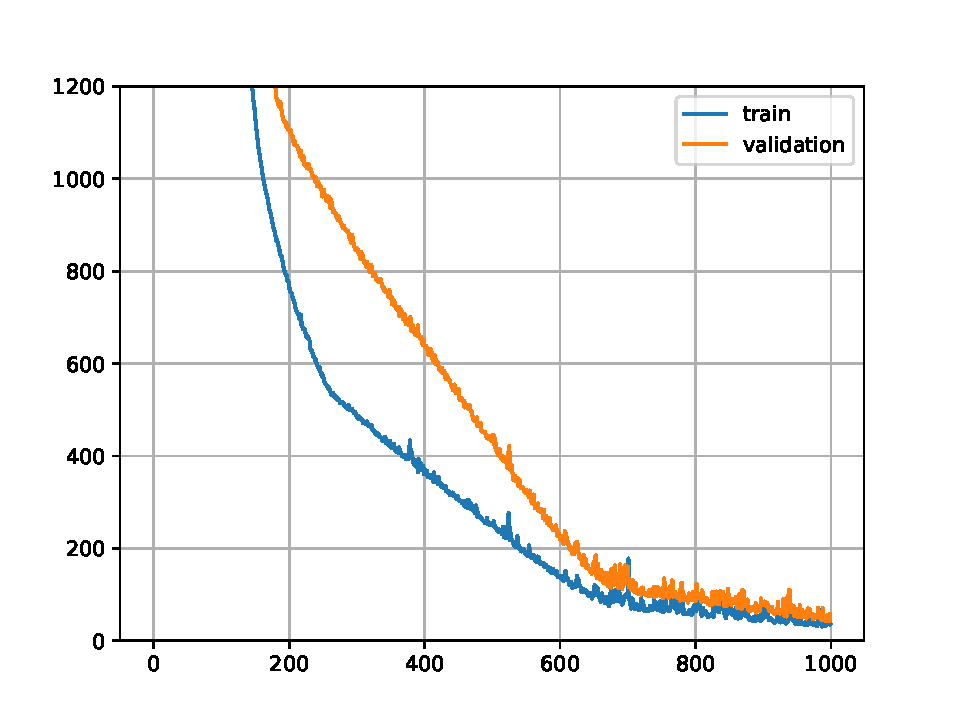
\includegraphics[width=\textwidth]{pics/figure_Credit_NN_nohidden_wd_loss.pdf}
    \caption{Loss on training and validation set during training epochs for the neural network with no hidden layers \& weight decay.}
    \label{fig:Credit_NN_nohidden_wd_loss}
\end{figure}

\begin{figure}
    \centering
    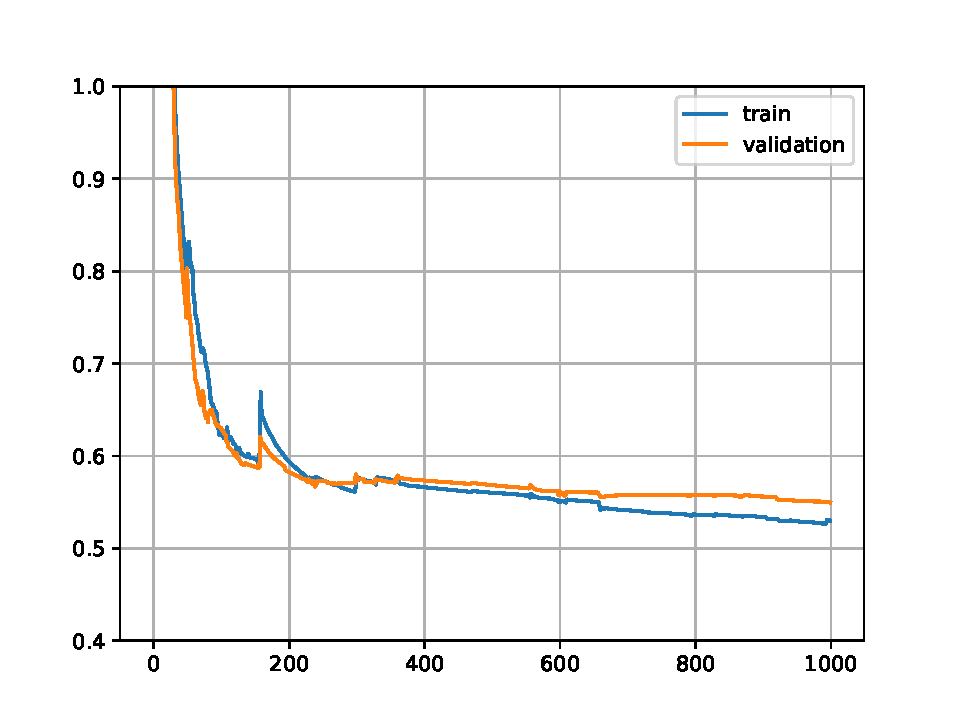
\includegraphics[width=\textwidth]{pics/figure_Credit_NN_1hidden_wd_loss.pdf}
    \caption{Loss on training and validation set during training epochs for the neural network with 1 hidden layers \& weight decay. }
    \label{fig:Credit_NN_1hidden_wd_loss}
\end{figure}


\begin{figure}
    \centering
    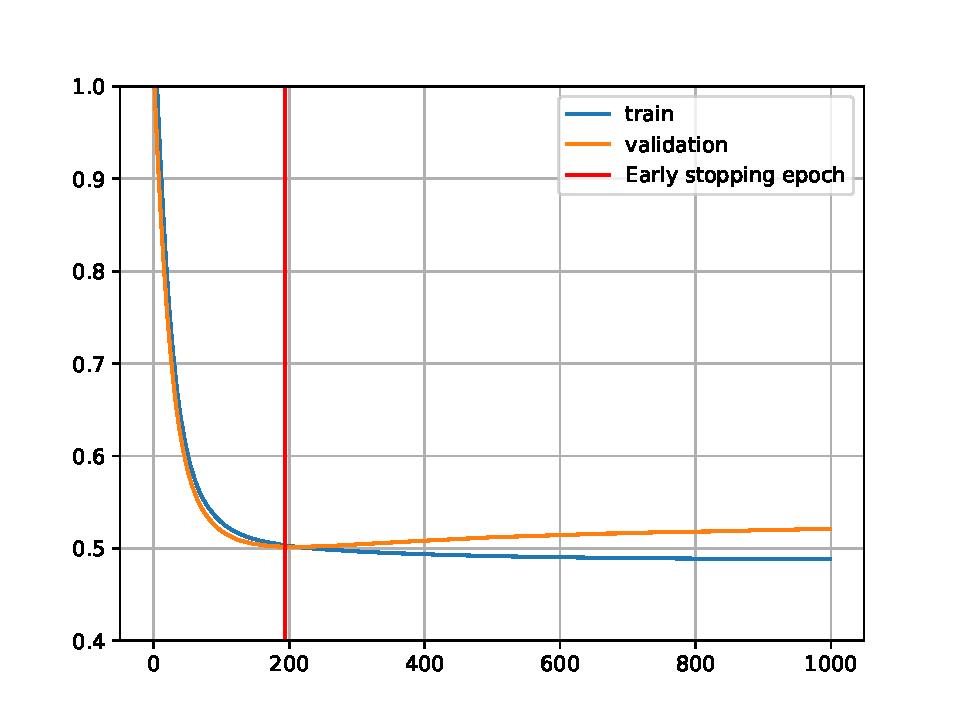
\includegraphics[width=\textwidth]{pics/figure_Credit_NN_1hidden_noreg_loss.pdf}
    \caption{Loss on training and validation set during training epochs for the neural network with 1 hidden layers \& no regularization. These losses are the same as for the network with 1 hidden layer and early stopping up to the stopping time on epoch 194, indicated by the red vertical line. It can be seen that validation loss is smoothly increasing, which is what made the early stopping algorithm indicate no further improvements in validation loss and stop the training, given the chosen patience of 0 epochs and $\delta_{\text{min}} = 0$.}
    \label{fig:Credit_NN_1hidden_noreg_loss}
\end{figure}
\clearpage
\subsection{Classification with Bayesian Neural Networks}
In this section we predict default probabilities with the Bayesian neural networks listed in table \ref{tab:credit_BNN_performance}. All these models are implemented with tanh activation function for the hidden layers and sigmoid for the output layer, as in the previous section with non-Bayesian neural network. All three models are implemented with a $\operatorname{Bernoulli}\lr{p}$ likelihood, where the bias $p$ is equal to the outputted probability of the network. The BNN with no hidden layers is used for comparing performance of the models to a simple Bayesian logistic regression. The BNN with one hidden layer has a $\mathcal{N}\lr{0,1}$ prior distribution placed on the network parameters. The hierarchical BNN with one hidden layer, has a $\mathcal{N}\lr{\mu,\sigma}$ prior for the network weights, where $\mu$ and $\sigma$ are distributed by a Cauchy and a half-normal distribution respectively, as in the regression evaluation. \\
\\
Sampling from the posterior distribution is performed using NUTS with three Markov chains, that runs in parallel, to avoid dependence between samples. For each chain we choose to draw 1500 samples, as running more than 1500 samples per chain resulted in the system exceeded its memory limit. Like before, we use a burn-in phase of 1000 samples for each chain, since we believe the Markov chains must have converged to the posterior by then. For the NUTS-algorithm we choose an
acceptance probability $\delta$ of $90\%$ and for all other inputs we use the default setting of \texttt{PyMC3}. Predictions are performed by sampling $1500 \times 3$ from the posterior predictive distribution and then take the mean across samples to make a single best guess for the default probability. \\
\\
In table \ref{tab:credit_BNN_performance} we see that both the BNN with one hidden layer and the BNN as a hierarchical model are performing better than the BNN with no hidden layers. This indicates that it is useful to use a neural network for predicting credit default probabilities compared to using Bayesian logistic regression. We see that the runtimes of the BNNs are much higher than the non-Bayesian models, and since we get the same results in terms of cross-entropy loss, it is not beneficial to use BNNs instead of NNs if one is only interested in getting the lowest loss pr. runtime.  \\

\begin{table} 
\caption{Performance measurement for Bayesian neural network models on credit card default data. The Python code used to implement these Bayesian neural networks can be seen in appendix \ref{app:Credit_BNN}.}
\label{tab:credit_BNN_performance}
\resizebox{\textwidth}{!}{%
    \begin{tabular}{|l|l|l|l|}
    \hline
    \multicolumn{1}{|c|}{{\cellcolor{ashgrey}{
     \textbf{Model}}}} & \multicolumn{1}{|c|}{{\cellcolor{ashgrey}{
     \textbf{Train cross-entropy loss}}}}       & \multicolumn{1}{|c|}{{\cellcolor{ashgrey}{
     \textbf{Test cross-entropy loss}}}} & \multicolumn{1}{|c|}{{\cellcolor{ashgrey}{
     \textbf{Runtime (s)}}}} \\ \hline
    No hidden layers  &  0.774  &  0.685   &    20.332      \\ \hline
    1 hidden layer &  0.523   &  0.539   &   1233.58       \\ \hline
    Hierarchical with 1 hidden layer  &  0.523  &   0.539  &   3640.28       \\ \hline
    \end{tabular}
}
\end{table}
\noindent
The benefits of the BNNs are instead found in the produced distribution of the predictive posterior. From a risk management perspective, this could be interesting to get an idea of the uncertainty of the models prediction of default probability. The mean probability of defaulting might be $45 \%$ for two different clients, but the uncertainty in this quantity might be significantly different. This uncertainty can be examined by taking a look at the posterior predictive distribution. In figure \ref{fig:ppc_credit} we have illustrated the posterior predictive distribution generated by the one hidden layer BNN for example 5, 11, 25 and 88 in the test dataset. We see that sometimes the model is quite confident about its predictions as in subfigure (c) and (d), but for other examples the uncertainty, expressed by the standard deviation of the distribution, is quite high like in subfigure (a) and (b). A bank could use this to decide not to give credit to a client if the uncertainty of the default probability is too high, like the client corresponding to subfigure (a) of figure \ref{fig:ppc_credit}.
\\
\\
In practice one might use the predicted default probabilities, that we use for our evaluation, to predict if the client will default or not. One can do this by classifying the most probable class, which means predicting default if the probability is more than $50 \%$.
This might however not be the most reasonable approach, if one prefers to wrongly classify one class more than the other. We might for example imagine that providing credit to a client that defaults next month would be much worse than denying a client that does not default next month. In this case it can make sense to choose another classification boundary than $50\%$. 
\\
\\
This classification boundary can be determined by the loss of wrongly predicting certain classes and can be set so that the expected loss do not exceed a certain value. Choosing a proper classification boundary for this case will however not be pursued further, as we performed our evaluation using the default probabilities instead of the labels, which would depend on the choice of such classification boundary.
  

\begin{figure}
    \centering
    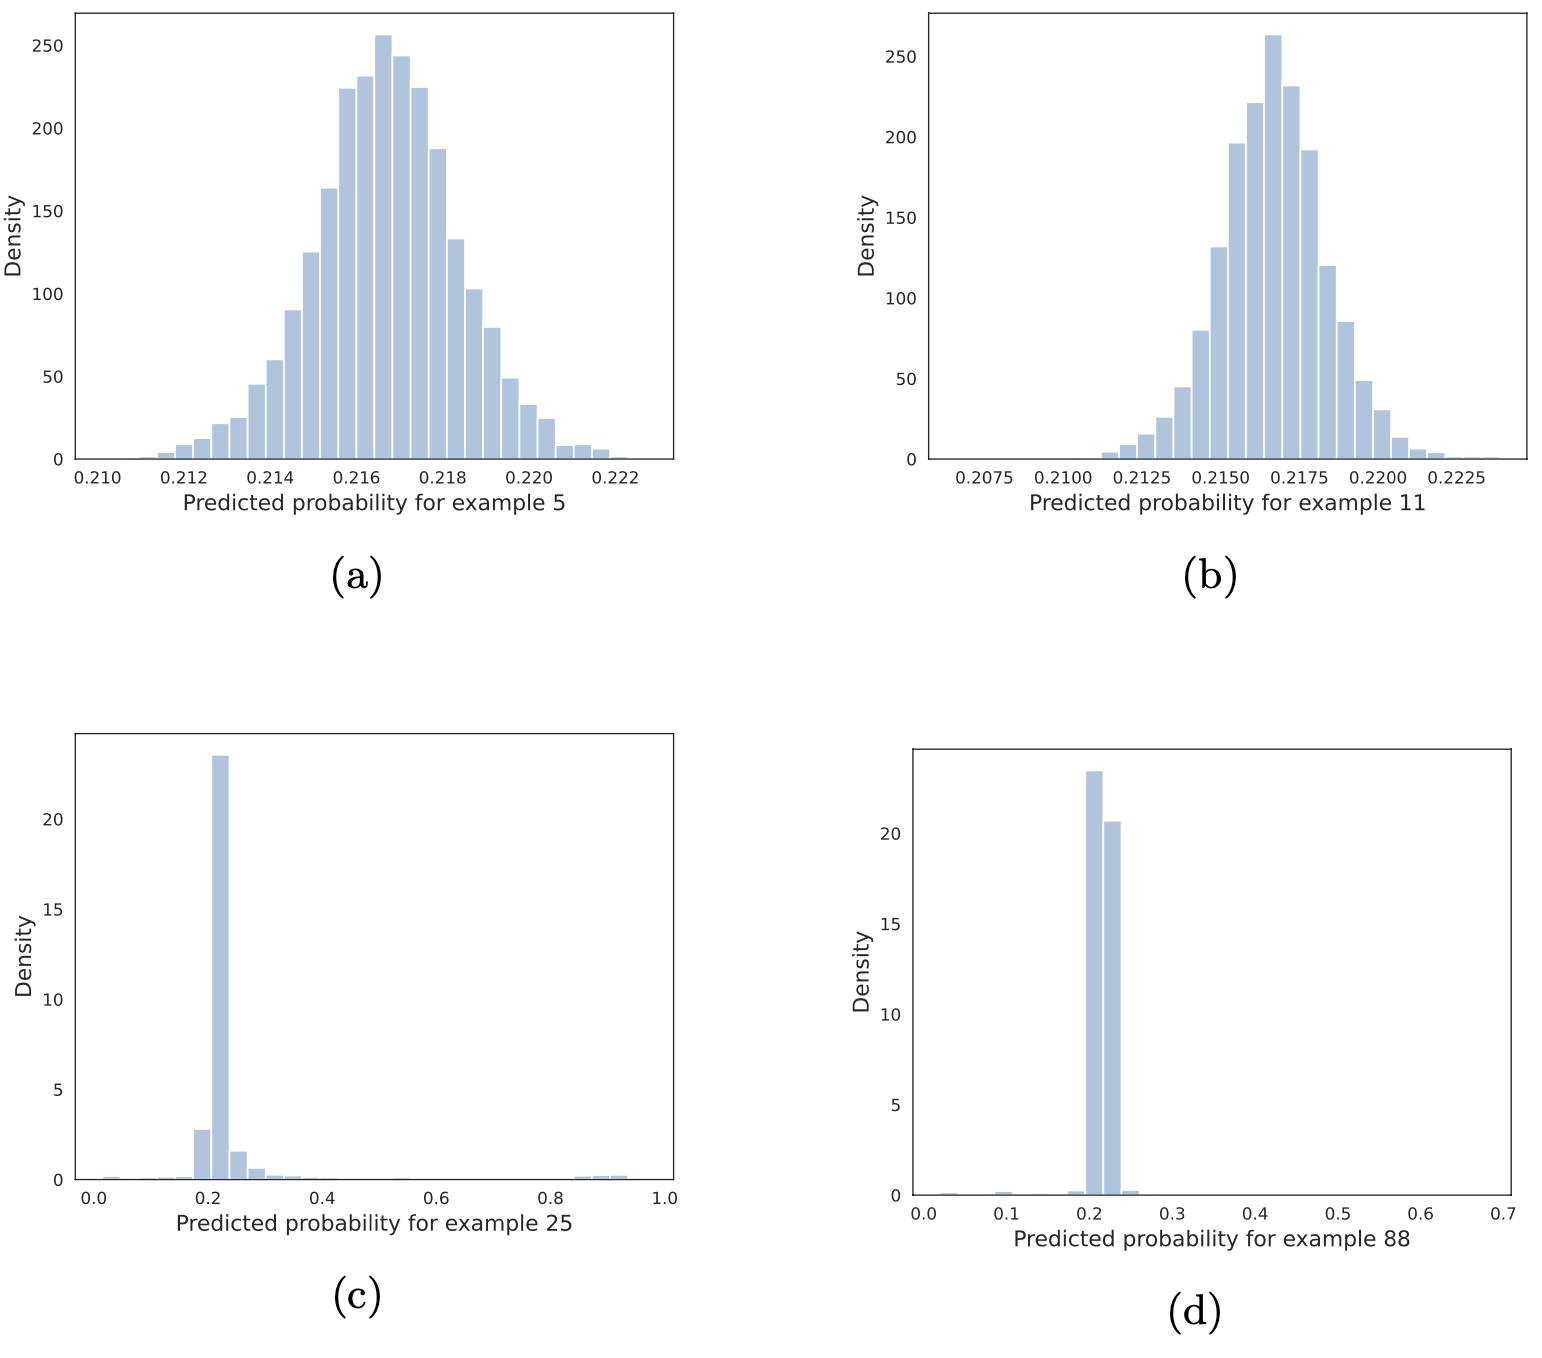
\includegraphics[width=\textwidth]{pics/post_pred_credit.png}
    \caption{A histogram of predictions generated by sampling from the posterior predictive distribution for example 5, 11, 25 and 88 in the test dataset. The predictions are based on the 1 hidden layer BNN model.}
    \label{fig:ppc_credit}
\end{figure}



\chapter{Conclusion}
In this thesis we have examined how Bayesian inference can be used in neural networks using Markov chain Monte Carlo sampling and how these and non-Bayesian neural networks perform regression and classification. The most essential difference between these two approaches of using neural networks is that Bayesian neural networks require a prior distribution for its weights and use sampling procedures to generate a distribution for its weights and predictions, while non-Bayesian neural networks use optimization algorithms, such as the gradient-based optimization algorithms described in section \ref{sec:gradient_optimization}, to learn a single estimate of the weights that result in predictions that provide the least amount of loss. 
\\
\\
The focal point of the examination of the Bayesian neural networks has been how to efficiently sample from the posterior distribution for the weights using Markov chain Monte Carlo methods. We analyzed this by first providing a simple example of a Bayesian neural network that took weights sampled from a prior and accepted them with a probability proportional to the likelihood of the produced results, a sort of rejections sampling illustrated by \cite{neal2012bayesian}. This provided the motivation for examining more efficient sampling methods such as the Markov chain Monte Carlo methods. One such method was the Metropolis algorithm that has the inefficiency of exploring the distribution with a random walk behavior. For this reason we examined the Hamiltonian Monte Carlo, which combine the principles of the Metropolis algorithm with Hamiltonian dynamics for a better exploration of the distribution. This turns out to have the inefficiency of sometimes performing "U-turns", meaning that it has the possibility of returning to the previous sample-point of the Markov chain and thus make highly correlated samples. 
The No-U-Turn Hamiltonian Monte Carlo is an extension to Hamiltonian Monte Carlo, which prevents such a U-turn and also make adaptive choices to the size and the number of steps taken by the Markov chain before sampling. We conclude our examination of Bayesian neural networks by covering the effect of the prior choice and by suggesting general schemes for choosing a prior distribution.
\\
\\
We end our thesis with an evaluation and illustration on how Bayesian and non-Bayesian neural networks work in practice. We do this with varying design choices to show how elements such as a hierarchical prior and different choice of regularization affects results. These different neural networks are applied to a regression task with the aim of predicting house prices and a classification task with the aim of predicting default probabilities of credit card clients. We furthermore show some of the benefits from the produced distributions of the predictive posterior from the Bayesian neural networks, and how to use these to evaluate models and make better predictions.
\chapter{Future work}
In this thesis we examined Bayesian neural network exclusively using Markov chain Monte Carlo methods. These methods are often computationally complex, especially in neural network where the posterior is high-dimensional due to number of neural network weights. Therefore it could have been interesting to look at methods that could be more easily scaled to large distributions. Methods such as variational Inference (\cite{VI}) has gained a lot of popularity due to its scalability to more complex models. Unlike Markov chain Monte Carlo methods, variational inference is not an exact method. Instead of sampling directly from the posterior the idea is to have a parametric distribution $q\lr{\boldsymbol{\phi}}$, called the variational distribution, to sample from instead. The parameters of the variational distribution are optimized in such a way that the variational distribution is as close as possible to the true posterior distribution in terms of a measure called the evidence lower bound. In this context it could have been interesting to look into the work by \cite{ADVI}, who has built an automatic differentiation variational inference algorithm, that can automatically optimize the parameters for the variational distribution. 
\\
\\
Another interesting way to design Bayesian neural networks is proposed by \cite{blundell2015weight} and is called Bayes-by-backprop, which is a variational inference methods combined with reparamitzation trick to ensure that backpropagation works as we described in section \ref{alg:back_prop}, but over the variational distribution parameters $\boldsymbol{\phi}$, which makes it possible to learn the variational distribution by using optimization algorithms like the ones described in section \ref{sec:gradient_optimization}. 
\\
\\
Another popular option worth examining is modelling uncertainty in neural networks by using dropout (\cite{srivastava2014dropout}) to approximate the variational distribution. \cite{mc_dropout} do this by using a type of ensemble learning, where they generate random predictions for test examples by the dropout method and interpret these as coming from a distribution. They call this method Monte Carlo dropout and states, that it produces faster results than both MCMC methods and variational inference. 






\bibliographystyle{agsm}
\nocite{*}
\bibliography{bibFile.bib}  % If you have some references, use BibTeX

\begin{appendices}

\section{Python code used for producing the over-underfitting example in figure \ref{fig:regr_example}} \label{app:overfitting}
\begin{lstlisting}
import numpy as np
import matplotlib.pyplot as plt
from sklearn.pipeline import Pipeline
from sklearn.preprocessing import PolynomialFeatures
from sklearn.linear_model import LinearRegression
from sklearn.model_selection import cross_val_score


def true_fun(X):
    return np.cos(1.5 * np.pi * X)


np.random.seed(0)

n_samples = 30
degrees = [1, 4, 15]

X = np.sort(np.random.rand(n_samples))
y = true_fun(X) + np.random.randn(n_samples) * 0.1

plt.figure(figsize=(14, 5))
for i in range(len(degrees)):
    ax = plt.subplot(1, len(degrees), i + 1)
    plt.setp(ax, xticks=(), yticks=())

    polynomial_features = PolynomialFeatures(degree=degrees[i],
                                             include_bias=False)
    linear_regression = LinearRegression()
    pipeline = Pipeline([("polynomial_features", polynomial_features),
                         ("linear_regression", linear_regression)])
    pipeline.fit(X[:, np.newaxis], y)

    # Evaluate the models using crossvalidation
    scores = cross_val_score(pipeline, X[:, np.newaxis], y,
                             scoring="neg_mean_squared_error", cv=10)

    X_test = np.linspace(0, 1, 100)
    plt.plot(X_test, pipeline.predict(X_test[:, np.newaxis]), label="Model")
    plt.plot(X_test, true_fun(X_test),
             label="True function", linestyle='dashed')
    plt.scatter(X, y, edgecolor='b', s=20, label="Samples")
    plt.xlabel("x")
    plt.ylabel("y")
    plt.xlim((0, 1))
    plt.ylim((-2, 2))
    plt.legend(loc="best")
    plt.title("Degree {}\nMSE_cv = {:.2e}(+/- {:.2e})".format(
        degrees[i], -scores.mean(), scores.std()))
plt.show()

\end{lstlisting}

\section{Python code for producing the activation functions in figure \ref{fig:act_funcs}} \label{app:act_funcs}

\begin{lstlisting}
import tensorflow as tf
import matplotlib.pyplot as plt

x = tf.linspace(-10., 10., 200)
y_sigmoid = tf.keras.activations.sigmoid(x)
y_tanh = tf.keras.activations.tanh(x)
y_relu = tf.keras.activations.relu(x)
y_elu = tf.keras.activations.elu(x)
y_step = x > 0

plt.plot(x, y_sigmoid, label='Sigmoid')
plt.plot(x, y_tanh, label=r'$tanh$')
plt.plot(x, y_relu, label='ReLU')
plt.plot(x, y_elu, label='ELU')
plt.plot(x, y_step, label='Step')
axes = plt.gca()
axes.set_ylim([-2, 2])
plt.xlabel('x')
plt.ylabel('g(x)')
plt.legend()
plt.savefig('act_func_fig.pdf')
plt.show()
\end{lstlisting}


\section{Python code for implementing the simple Bayesian neural network illustrated in figure \ref{fig:simple_BNN}} \label{app:simple_BNN}
\begin{lstlisting}
#import random as rn
import matplotlib.pyplot as plt
import numpy as np
import tensorflow as tf
import tensorflow_probability as tfp
tfd = tfp.distributions

# -------------------------------- Creating sin-data -------------------------------


def true_fun(x):
    return np.sin(3 * x)  # np.sin(1.5 * np.pi * x)


np.random.seed(42)
n_x = 6
x_train = np.sort(np.random.rand(n_x))
y_train = true_fun(x_train)  


# --------------------- Build and compile neural net -------------------------------

model = tf.keras.models.Sequential([
    tf.keras.layers.Dense(16, input_shape=([1, ]), activation='tanh'),
    tf.keras.layers.Dense(1, activation='tanh')
])
model.summary()


# --------------------- Sample weights through neural networks with acceptance-prop equal to likelihood ----------------------

n_NN = 10**5
weight_list = []
likelihood_list = []
sigma_k = 0.1  # sd of assumed gauss P(y \mid x), Neal's eq 1.8, Neal uses 0.1
tf.random.set_seed(42)
# Sample neural networks and save their likelihood and weights
for i in range(n_NN):
    print(i)
    # sample weights and set them to hidden layer "dense" and output layer "dense_1"
    for layer in model.layers:
        if layer.name == "dense":
            layer.set_weights([np.random.normal(0, 8, size=w.shape)
                               for w in layer.get_weights()])
        if layer.name == "dense_1":
            layer.set_weights([np.random.normal(
                0, 1/np.sqrt(16), size=w.shape) for w in layer.get_weights()])
    # save weights in list
    weight_list.append(model.get_weights())
    # Calculate gauss likelihood of y_train given weights and x_train, Neal's eq 1.11
    mean = model.predict(x_train)
    gauss = tfd.Normal(loc=mean, scale=sigma_k)
    likelihood = 1
    for j in range(n_x):
        likelihood *= gauss[j].prob(y_train[j])
    likelihood_list.append(likelihood)

# Normalize likelihood to max prob is 1
if max(likelihood_list) != 0:
    likelihood_list = likelihood_list/max(likelihood_list)

# Accept model with prob equal to normalized likelihood
accepted_weights = []
accepted_likelihood = []
for i in range(len(likelihood_list)):
    uniform_dist = tfd.Uniform(0, 1)
    if likelihood_list[i] >= uniform_dist.sample():
        accepted_weights.append(weight_list[i])
        accepted_likelihood.append(likelihood_list[i])


# --------------------- Use sampled weights for predicting y's ----------------------
x_pred = tf.linspace(0.0, 1, 200)
y_pred = []
for i in range(len(accepted_weights)):
    model.set_weights(accepted_weights[i])
    y_pred.append(model.predict(x_pred))

# mean y_pred
mean_y_pred = np.array(y_pred).mean(axis=0)

y_pred_std = np.array(y_pred).std(axis = 0)
# Lower std-line
lower_std = mean_y_pred - y_pred_std 
# Upper std-line
upper_std = mean_y_pred + y_pred_std

# --------------------- Plot of BNN results ----------------------
plt.scatter(x_train, y_train,
            edgecolor='b', s=40, label="Datapoint")
for i in range(len(y_pred)):
    plt.plot(x_pred, y_pred[i], color='k', linestyle='dashed')
plt.plot(x_pred, mean_y_pred, color='coral', label="Average prediction")
plt.fill_between(x_pred, lower_std.flatten() , upper_std.flatten() , color='b', alpha=.1)
plt.xlabel('x')
plt.ylabel('y')
plt.legend()
plt.savefig('figure_simple_BNN.pdf')
plt.show()

\end{lstlisting}



\section{Python code for Metropolis implementation used for producing figure \ref{fig:MH_sampling} }\label{app:MH_code}
\begin{lstlisting}
# # ----------------------------- IMPORTS ---------------------------

import numpy as np
import scipy.stats as ss
import matplotlib.pyplot as plt

# # ----------------------------- Defining functions ---------------------------
# Defining target probability
def p(x):
    sigma = np.array([[1, 0.6], [0.6, 1]])  # Covariance matrix
    return ss.multivariate_normal.pdf(x, cov=sigma)

# # ----------------------------- Sampling  ---------------------------
samples = np.zeros((1000, 2))
np.random.seed(42)

x = np.array([7, 0])
for i in range(1000):
    samples[i] = x
    # Gaussian proposal for symmetry
    x_prime = np.random.multivariate_normal(mean=x, cov=np.eye(2), size=1).flatten()
    acceptance_prob = min(1, (p(x_prime) )/ (p(x)))
    u = np.random.uniform(0, 1)
    if u <= acceptance_prob:
        x = x_prime
    else:
        x = x

# # ----------------------------- Vizualising  ---------------------------
 
# For vizualising normal contours       
X, Y = np.mgrid[-3:3:0.05, -3:3:0.05]    
X, Y = np.mgrid[-3:3:0.05, -3:3:0.05]
XY = np.empty(X.shape + (2,))
XY[:,:,0] = X; XY[:,:,1] = Y
target_distribution = ss.multivariate_normal(mean=[0,0], cov=[[1, 0.6],[0.6, 1]])


plt.subplot(2, 2, 1) # row 1, col 2 index 1
plt.contour(X, Y, target_distribution.pdf(XY),cmap=plt.cm.Blues)
plt.ylim(-3,5)
plt.xlim(-3,8)
plt.subplot(2, 2, 2) # index 2
plt.plot(samples[0:100,0], samples[0:100,1], 'ro-', color="navy", linewidth=.2, markersize=.7,label="First 100 samples")
plt.contour(X, Y, target_distribution.pdf(XY),cmap=plt.cm.Blues)
plt.legend(loc="upper right",fontsize=9)
plt.ylim(-3,5)
plt.xlim(-3,8)
plt.subplot(2, 2, 3) # index 3
plt.plot(samples[0:200,0], samples[0:200,1], 'ro-', color="navy", linewidth=.2, markersize=.7,label="First 200 samples")
plt.contour(X, Y, target_distribution.pdf(XY),cmap=plt.cm.Blues)
plt.legend(loc="upper right",fontsize=9)
plt.ylim(-3,5)
plt.xlim(-3,8)
plt.subplot(2, 2, 4) # index 4
plt.plot(samples[0:300,0], samples[0:300,1], 'ro-', color="navy", linewidth=.2, markersize=.7, label="First 300 samples")
plt.contour(X, Y, target_distribution.pdf(XY),cmap=plt.cm.Blues)
plt.legend(loc="upper right",fontsize=9)
plt.ylim(-3,5)
plt.xlim(-3,8)
plt.savefig("metro_example.pdf")
plt.show()

\end{lstlisting}





\section{Python packages and specification for computer doing the evaluations in chapter \ref{chap:eval_NN}} \label{app:specs}
The code ran on a virtual machine for the Linux distribution Ubuntu 20.04.2 LTS. The virtual machine used VMWare Workstation 16.1.1 on a native Windows 10 64-bit version 2004. The hardware used is
\begin{itemize}
    \item GPU: NVidia GeForce GTX 970
    \item RAM allocated to virtual machine: 9.5 GB
    \item Processor: Intel® Core™ i5-6600K CPU @ 3.50GHz × 4
    \item A harddrive allocated only to this virtual machine with free space of 427 GB
\end{itemize}
The packages required for reproducing the evalutions are 
\begin{itemize}
    \item \texttt{PyMC3}==3.11.2
    \item \texttt{Theano}==1.1.2
    \item \texttt{Arviz}==0.11.2
    \item \texttt{Numpy}==1.19.5
    \item \texttt{tensorflow}==2.4.1
    \item \texttt{tensorflow\_probability}==0.12.2
    \item \texttt{sklearn}==0.24.2
    \item \texttt{numpy}==1.19.5
    \item \texttt{seaborn}==0.11.1
    \item \texttt{matplotlib.pyplot}==3.4.1
\end{itemize}



\section{Python code for the neural networks in table \ref{tab:Boston_NN_performance}} \label{app:Boston_NN}
The network with with early stopping is performed using the code
\begin{lstlisting}
import tensorflow as tf
import numpy as np
import matplotlib.pyplot as plt
from keras.datasets import boston_housing
import time


tf.random.set_seed(40)

# ----------------------------- Prepare data ---------------------
(X_train, y_train), (X_test, y_test) = boston_housing.load_data(seed=3030)

# ----------------------------- Neural Network ---------------------
n_hidden = 10

model = tf.keras.Sequential([
    tf.keras.Input((13, ), name='feature'),
    tf.keras.layers.Dense(n_hidden, activation=tf.nn.relu),
    tf.keras.layers.Dense(1)
])
model.summary()

# Early stopping
es = tf.keras.callbacks.EarlyStopping(
    monitor='val_loss', mode='min', patience=10, min_delta=0.1)

start_time = time.time()
# Compile, train, and evaluate.
model.compile(optimizer='adam',
              loss='mean_squared_error',
              metrics=['mse'])
history = model.fit(X_train, y_train, epochs=300,
                    validation_split=0.3, callbacks=[es])

print("The algorithm ran", len(history.history['loss']), "epochs")


# ----------------------------- Overfitting? ---------------------
train_acc = model.evaluate(X_train, y_train, verbose=0)[-1]
test_acc = model.evaluate(X_test, y_test, verbose=0)[-1]
print("--- %s seconds ---" % (time.time() - start_time))
print('Train: %.3f, Test: %.3f' % (train_acc, test_acc))

plt.plot(history.history['loss'], label='train')
plt.plot(history.history['val_loss'], label='validation')
plt.legend()
plt.grid()
plt.show()

\end{lstlisting}
The networks not using early stopping and their visualization of train and validation loss in figure \ref{fig:Boston_NN_nohidden_wd_loss}, figure \ref{fig:Boston_NN_1hidden_wd_loss} and figure \ref{fig:Boston_NN_1hidden_noreg_loss} are produced using the code
\begin{lstlisting}
import tensorflow as tf
import numpy as np
import matplotlib.pyplot as plt
from keras.datasets import boston_housing
import time
from keras.regularizers import l2

tf.random.set_seed(40)
# ----------------------------- Prepare data ----------------------
(X_train, y_train), (X_test, y_test) = boston_housing.load_data(seed=3030)


# ----------------------------- Neural Network --------------------
reg_const = 0.3
n_hidden = 10

model = tf.keras.Sequential([
    tf.keras.Input((13, ), name='feature'),
    tf.keras.layers.Dense(n_hidden, activation=tf.nn.relu, kernel_regularizer=l2(
        reg_const), bias_regularizer=l2(reg_const)),
    tf.keras.layers.Dense(1, kernel_regularizer=l2(
        reg_const), bias_regularizer=l2(reg_const))
])
model.summary()

start_time = time.time()
# Compile, train, and evaluate.
model.compile(optimizer='adam',
              loss='mean_squared_error',
              metrics=['mse'])
history = model.fit(X_train, y_train, epochs=300, validation_split=0.3)
model.evaluate(X_test, y_test)


# ----------------------------- Overfitting? --------------------
train_acc = model.evaluate(X_train, y_train, verbose=0)[-1]
test_acc = model.evaluate(X_test, y_test, verbose=0)[-1]
print("--- %s seconds ---" % (time.time() - start_time))
print('Train: %.3f, Test: %.3f' % (train_acc, test_acc))

plt.plot(history.history['loss'], label='Train')
plt.plot(history.history['val_loss'], label='Validation')
plt.legend()
plt.grid()
plt.ylabel('Loss')
plt.xlabel('Epochs')
plt.ylim(0, 200)
plt.savefig('figure_Boston_NN_1hidden_wd_loss.pdf')
plt.show()

\end{lstlisting}
where the network with no hidden layers are produced by removing the line \begin{lstlisting}
tf.keras.layers.Dense(n_hidden, activation=tf.nn.relu, kernel_regularizer=l2(
        reg_const), bias_regularizer=l2(reg_const))
\end{lstlisting}
and the network with 1 hidden layer and no regularization is produced by removing the regularization arguments \texttt{kernel\_regularizer} and \texttt{bias\_regularizer} in 
\begin{lstlisting}
tf.keras.layers.Dense(n_hidden, activation=tf.nn.relu, kernel_regularizer=l2(
        reg_const), bias_regularizer=l2(reg_const)),
    tf.keras.layers.Dense(1, kernel_regularizer=l2(
        reg_const), bias_regularizer=l2(reg_const))
\end{lstlisting}




\section{Python code for the Bayesian neural networks in table \ref{tab:Boston_BNN_performance}} \label{app:Boston_BNN}
The Bayesian neural network with hierarchical model is implemented by the following code
\begin{lstlisting}
# # ----------------------------- IMPORTS -----------------------
import sys
import time
from keras.datasets import boston_housing
from sklearn import metrics
import numpy as np 
import pymc3 as pm
import theano
import arviz as az
from arviz.utils import Numba
import theano.tensor as tt
Numba.disable_numba()
Numba.numba_flag
floatX = theano.config.floatX
import seaborn as sns
sns.set_style("white")
import tensorflow as tf


# Ignore warnings - NUTS provide many runtimeWarning
import warnings
warnings.filterwarnings("ignore", category=RuntimeWarning)

tf.random.set_seed(42)
# # ----------------------------- Loading Boston data --------------
(X_train, y_train), (X_test, y_test) = boston_housing.load_data(seed=3030)

#pad Xs with 1's to add bias
ones_train=np.ones(X_train.shape[0])
ones_test=np.ones(X_test.shape[0])
X_train=np.insert(X_train,0,ones_train,axis=1)
X_test=np.insert(X_test,0,ones_test,axis=1)


# # ----------------------------- Implementing a BNN function -----

def construct_bnn(ann_input, ann_output, n_hidden):
    # Initialize random weights between each layer
    init_1 = np.random.randn(X_train.shape[1], n_hidden).astype(floatX)*.1
    init_out = np.random.randn(n_hidden,1).astype(floatX)*.1
    with pm.Model() as bayesian_neural_network:
        ann_input = pm.Data("ann_input", X_train)
        ann_output = pm.Data("ann_output", y_train)
      
    # prior on hyper parameters for weight 1
        #mu1 = pm.Normal('mu1',shape=(X_train.shape[1], n_hidden), mu=0, sigma=1)
        mu1 = pm.Cauchy('mu1',shape=(X_train.shape[1], n_hidden), alpha=0, beta=1)
        sigma1 = pm.HalfNormal('sigma1',shape=(X_train.shape[1], n_hidden), sigma=1) 
        
    # Input -> Layer 1
        weights_1 = pm.Normal('w_1', mu=mu1, sd=sigma1,
                          shape=(X_train.shape[1], n_hidden),
                          testval=init_1)
        acts_1 = pm.Deterministic('activations_1', tt.nnet.relu(tt.dot(ann_input, weights_1)))
    
    # prior on hyper parameters for weight_out 
        mu_out = pm.Cauchy('mu_out',shape=(n_hidden, 1), alpha=0, beta=1)
        sigma_out = pm.HalfNormal('sigma_out',shape=(n_hidden, 1), sigma=1) 
    
    # Layer 1 -> Output Layer
        weights_out = pm.Normal('w_out', mu=mu_out, sd=sigma_out,
                            shape=(n_hidden, 1),
                            testval=init_out)
        acts_out = pm.Deterministic('activations_out',tt.dot(acts_1, weights_out))
        

    #Define likelihood
        out = pm.Normal('out', mu=acts_out[:,0], sd=1, observed=ann_output)        
            
    return bayesian_neural_network


# # ---------------- Sampling from posterior ---------
# Start time
tic = time.perf_counter() # for timing
bayesian_neural_network_NUTS = construct_bnn(X_train, y_train, n_hidden=10)

# Sample from the posterior using the NUTS samplper
with bayesian_neural_network_NUTS:
    trace = pm.sample(draws=3000, tune=1000, chains=3,target_accept=.90)
    

# # ------------------ Making predictions on training data ---------
ppc1=pm.sample_posterior_predictive(trace, model=bayesian_neural_network_NUTS)

# Taking the mean over all samples to generate a prediction
y_train_pred = ppc1['out'].mean(axis=0)


# Replace shared variables with testing set
pm.set_data(new_data={"ann_input": X_test, "ann_output": y_test}, model=bayesian_neural_network_NUTS)



# # ---------------- Making predictions on test data ------
ppc2 = pm.sample_posterior_predictive(trace, model=bayesian_neural_network_NUTS)

# Taking the mean over all samples to generate a prediction
y_test_pred = ppc2['out'].mean(axis=0)

# End time
toc = time.perf_counter()
print(f"Run time {toc - tic:0.4f} seconds")

# Printing the performance measures
print('MSE (NUTS) on training data:', metrics.mean_squared_error(y_train, y_train_pred))
print('MSE (NUTS) on test data:', metrics.mean_squared_error(y_test, y_test_pred))

\end{lstlisting}
The Bayesian neural network with one hidden layer is implemented by the following code
\begin{lstlisting}
# # ----------------------------- IMPORTS -------------------
import sys
import time
from keras.datasets import boston_housing
from sklearn import metrics
import numpy as np 
import pymc3 as pm
import theano
import arviz as az
from arviz.utils import Numba
import theano.tensor as tt
Numba.disable_numba()
Numba.numba_flag
floatX = theano.config.floatX
# seaborn for vizualzing 
import seaborn as sns
sns.set_style("white")
import matplotlib.pyplot as plt
import tensorflow as tf
# # ----------------------------- Print versions -------------

print("Running on Python version %s" % sys.version)
print(f"Running on PyMC3 version{pm.__version__}")
print("Running on Theano version %s" % theano.__version__)
print("Running on Arviz version %s" % az.__version__)
print("Running on Numpy version %s" % np.__version__)

# Ignore warnings - NUTS provide many runtimeWarning
import warnings
warnings.filterwarnings("ignore", category=RuntimeWarning)

tf.random.set_seed(42)
# # ----------------------------- Loading Boston data ------------
(X_train, y_train), (X_test, y_test) = boston_housing.load_data(seed=3030)

#pad Xs with 1's to add bias
ones_train=np.ones(X_train.shape[0])
ones_test=np.ones(X_test.shape[0])
X_train=np.insert(X_train,0,ones_train,axis=1)
X_test=np.insert(X_test,0,ones_test,axis=1)


# # ----------------------------- Implementing a BNN function ------

def construct_bnn(ann_input, ann_output, n_hidden, prior_std):
    # Initialize random weights between each layer
    init_1 = np.random.randn(X_train.shape[1], n_hidden).astype(floatX)*prior_std
    init_out = np.random.randn(n_hidden,1).astype(floatX)*prior_std

    with pm.Model() as bayesian_neural_network:
        ann_input = pm.Data("ann_input", X_train)
        ann_output = pm.Data("ann_output", y_train)
        
    # Input -> Layer 1
        weights_1 = pm.Normal('w_1', mu=0, sd=prior_std,
                          shape=(X_train.shape[1], n_hidden),
                          testval=init_1)
        acts_1 = tt.nnet.relu(tt.dot(ann_input, weights_1))

    # Layer 1 -> Output Layer
        weights_out = pm.Normal('w_out', mu=0, sd=prior_std,
                            shape=(n_hidden, 1),
                            testval=init_out)
        acts_out = tt.dot(acts_1, weights_out)
        

    #Define likelihood
        out = pm.Normal('out', mu=acts_out[:,0], sd=1, observed=ann_output)        
            
    return bayesian_neural_network


# # ----------------------------- Sampling from posterior -------
# Start time
tic = time.perf_counter() # for timing
bayesian_neural_network_NUTS = construct_bnn(X_train, y_train, n_hidden=10, prior_std=.1)

# Sample from the posterior using the NUTS samplper
with bayesian_neural_network_NUTS:
    trace = pm.sample(draws=3000, tune=1000, chains=3,target_accept=.9, random_seed=42)
    

# # ------------------ Making predictions on training data --------
ppc1=pm.sample_posterior_predictive(trace, model=bayesian_neural_network_NUTS, random_seed=42)

# Taking the mean over all samples to generate a prediction
y_train_pred = ppc1['out'].mean(axis=0)


# Replace shared variables with testing set
pm.set_data(new_data={"ann_input": X_test, "ann_output": y_test}, model=bayesian_neural_network_NUTS)



# # ------------------- Making predictions on test data ------
ppc2 = pm.sample_posterior_predictive(trace, model=bayesian_neural_network_NUTS, random_seed=42)

# Taking the mean over all samples to generate a prediction
y_test_pred = ppc2['out'].mean(axis=0)

# End time
toc = time.perf_counter()
print(f"Run time {toc - tic:0.4f} seconds")

# Printing the performance measures
print('MSE (NUTS) on training data:', metrics.mean_squared_error(y_train, y_train_pred))
print('MSE (NUTS) on test data:', metrics.mean_squared_error(y_test, y_test_pred))


# -------------------------------- Plots --------------------
# Vizualize uncertainty
# Define examples for which you want to examine the posterior predictive:
example_vec=np.array([1,2,4,9,10,11,15,16,22,24,27,28,30,44,55,62,68,72,84,93])
for example in example_vec:
    plt_hist_array=np.array(ppc2['out'])
    plt.hist(plt_hist_array[:,example], density=1, color="lightsteelblue", bins=30)
    plt.xlabel(f"Predicted value for example {example}",fontsize=13)
    plt.ylabel("Density",fontsize=13)
    plt.savefig(f'Python_code/Boston_BNN_1hidden_postpred_{example}.pdf')
    plt.show()
\end{lstlisting}
where the network with no hidden layers is implemented by replacing the lines
\begin{lstlisting}
# Input -> Layer 1
    weights_1 = pm.Normal('w_1', mu=0, sd=prior_std,
                    shape=(X_train.shape[1], n_hidden),
                    testval=init_1)
    acts_1 = tt.nnet.relu(tt.dot(ann_input, weights_1))

# Layer 1 -> Output Layer
    weights_out = pm.Normal('w_out', mu=0, sd=prior_std,
                    shape=(n_hidden, 1),
                    testval=init_out)
    acts_out = tt.dot(acts_1, weights_out)
\end{lstlisting}
with
\begin{lstlisting}
 # Input layer -> Output layer
        weights_out = pm.Normal('w_out', mu=0, sd=prior_std,
        shape=(X_train.shape[1], 1), testval=init_out)
    acts_out = pm.Deterministic(
        'activations_out', tt.dot(ann_input, weights_out))
\end{lstlisting}


\section{Python code for the neural networks in table \ref{tab:credit_NN_performance}} \label{app:Credit_NN}
The neural network with early stopping is performed using the code
\begin{lstlisting}
 import time
import tensorflow as tf
import numpy as np
import matplotlib.pyplot as plt
import pandas as pd
from sklearn.model_selection import train_test_split
import seaborn as sns

tf.random.set_seed(40)
# ----------------------------- Prepare data -------------------
credit_data = pd.read_csv(
    "Python_code/data/UCI_Credit_Card.csv", encoding="utf-8", index_col=0)
credit_data.head()

# Data to numpy
data = np.array(credit_data)

# Extract labels
data_X = data[:, 0:23]
data_y = data[:, 23]


# # -------------------------- Subsamling credit data -------
X_train, X_test, y_train, y_test = train_test_split(
    data_X, data_y, test_size=0.30, random_state=3030)

N = 300
N_test = 100
X_train = X_train[0:N, :]
y_train = y_train[0:N]
X_test = X_test[0:N_test, :]
y_test = y_test[0:N_test]


# ------------------------- Neural Network ---------------

model = tf.keras.Sequential([
    tf.keras.Input((23, ), name='feature'),
    tf.keras.layers.Dense(10, activation=tf.nn.tanh),
    tf.keras.layers.Dense(1, activation=tf.nn.sigmoid)
])
model.summary()

# Early stopping
es = tf.keras.callbacks.EarlyStopping(
    monitor='val_loss', mode='min', patience=0, min_delta=0)

start_time = time.time()

# Compile, train, and evaluate.
model.compile(optimizer='adam',
              loss='binary_crossentropy',
              metrics=['binary_crossentropy'])
history = model.fit(X_train, y_train,  validation_split=0.3,
                    epochs=1000, callbacks=[es])
print("The algorithm ran", len(history.history['loss']), "epochs")

print("--- %s seconds ---" % (time.time() - start_time))


# ------------------------- Overfitting? ----------------
train_acc = model.evaluate(X_train, y_train, verbose=0)[-1]
test_acc = model.evaluate(X_test, y_test, verbose=0)[-1]
print('Train: %.3f, Test: %.3f' % (train_acc, test_acc))

# taking mean of summed cross-entropy loss
train_loss = np.array(history.history['loss'])
val_loss = np.array(history.history['val_loss'])

plt.plot(train_loss, label='train')
plt.plot(val_loss, label='validation')
plt.legend()
plt.grid()
plt.show()

\end{lstlisting}
The networks not using early stopping and their visualization of train and validation loss in figure \ref{fig:Credit_NN_nohidden_wd_loss}, \ref{fig:Credit_NN_1hidden_wd_loss} and figure \ref{fig:Credit_NN_1hidden_noreg_loss} are produced using the code
\begin{lstlisting}
from keras.regularizers import l2
import time
import tensorflow as tf
import numpy as np
import matplotlib.pyplot as plt
import pandas as pd
from sklearn.model_selection import train_test_split
import seaborn as sns
start_time = time.time()
tf.random.set_seed(40)

# ----------------------------- Prepare data ----------------
credit_data = pd.read_csv(
    "Python_code/data/UCI_Credit_Card.csv", encoding="utf-8", index_col=0)
credit_data.head()

# Data to numpy
data = np.array(credit_data)

# Extract labels
data_X = data[:, 0:23]
data_y = data[:, 23]

# # ----------------------------- Subsamling credit data ------
X_train, X_test, y_train, y_test = train_test_split(
    data_X, data_y, test_size=0.30, random_state=3030)

N = 300
N_test = 100
X_train = X_train[0:N, :]
y_train = y_train[0:N]
X_test = X_test[0:N_test, :]
y_test = y_test[0:N_test]

# ----------------------------- Neural Network ----------------
reg_const = 0.1
n_hidden = 10

model = tf.keras.Sequential([
    tf.keras.Input((23, ), name='feature'),
    tf.keras.layers.Dense(n_hidden, activation=tf.nn.tanh, kernel_regularizer=l2(
        reg_const), bias_regularizer=l2(reg_const)),
    tf.keras.layers.Dense(1, activation=tf.nn.sigmoid, kernel_regularizer=l2(
        reg_const), bias_regularizer=l2(reg_const))
])
model.summary()

# Compile, train, and evaluate.
val_ratio = 0.3
model.compile(optimizer='adam',
              loss='binary_crossentropy',
              metrics=['binary_crossentropy'])
history = model.fit(X_train, y_train, epochs=1000,
                    validation_split=val_ratio)

model.evaluate(X_test, y_test)

print("--- %s seconds ---" % (time.time() - start_time))


# ----------------------------- Overfitting? ----------------

train_acc = model.evaluate(X_train, y_train, verbose=0)[-1]
test_acc = model.evaluate(X_test, y_test, verbose=0)[-1]
print('Train: %.3f, Test: %.3f' % (train_acc, test_acc))

# taking mean of summed cross-entropy loss
train_loss = np.array(history.history['loss'])
val_loss = np.array(history.history['val_loss'])

plt.plot(train_loss, label='train')
plt.plot(val_loss, label='validation')
plt.legend()
plt.grid()
plt.ylim(0.4, 1)
plt.savefig('Python_code/figure_Credit_NN_1hidden_wd_loss.pdf')
plt.show()

\end{lstlisting}
where the network with no hidden layers are produced by removing the line
\begin{lstlisting}
 tf.keras.layers.Dense(n_hidden, activation=tf.nn.tanh, kernel_regularizer=l2(
        reg_const), bias_regularizer=l2(reg_const)),
\end{lstlisting}
and the network with 1 hidden layer and no regularization is produced by removing the regularization arguments \texttt{kernel\_regularizer} and \texttt{bias\_regularizer} in 
\begin{lstlisting}
tf.keras.layers.Dense(n_hidden, activation=tf.nn.tanh, kernel_regularizer=l2(
        reg_const), bias_regularizer=l2(reg_const)),
tf.keras.layers.Dense(1, activation=tf.nn.sigmoid, kernel_regularizer=l2(
        reg_const), bias_regularizer=l2(reg_const))
\end{lstlisting}

\section{Python code for the Bayesian neural networks in table \ref{tab:credit_BNN_performance}} \label{app:Credit_BNN}
The Bayesian neural network with hierarchical model is implemented by the following code
\begin{lstlisting}
# # ----------------------------- IMPORTS -----------------
import warnings
from sklearn.metrics import accuracy_score, log_loss
import matplotlib.pyplot as plt
import seaborn as sns
import tensorflow as tf
import sys
import time
import numpy as np
from sklearn.model_selection import train_test_split
import pandas as pd
import pymc3 as pm
import theano
import arviz as az
from arviz.utils import Numba
import theano.tensor as tt
from scipy.stats import mode
Numba.disable_numba()
Numba.numba_flag
floatX = theano.config.floatX
sns.set_style("white")


# # ----------------------------- Print versions -----------------
print("Running on Python version %s" % sys.version)
print(f"Running on PyMC3 version{pm.__version__}")
print("Running on Theano version %s" % theano.__version__)
print("Running on Arviz version %s" % az.__version__)
print("Running on Numpy version %s" % np.__version__)

# Ignore warnings - NUTS provide many runtimeWarning
warnings.filterwarnings("ignore", category=RuntimeWarning)

tf.random.set_seed(42)


# # ----------------------------- Loading credit data ---
credit_data = pd.read_csv("Python_code/data/UCI_Credit_Card.csv",
                          encoding="utf-8", index_col=0, delimiter=",")
credit_data.head()
# Data to numpy
data = np.array(credit_data)
# seperating labels from features
data_X = data[:, 0:23]
data_y = data[:, 23]


# # ----------------------------- Subsamling credit data --------
X_train, X_test, y_train, y_test = train_test_split(
    data_X, data_y, test_size=0.30, random_state=3030)

N = 300
N_test = 100
X_train = X_train[0:N, :]
y_train = y_train[0:N]
X_test = X_test[0:N_test, :]
y_test = y_test[0:N_test]


# pad Xs with 1's to add bias
ones_train = np.ones(X_train.shape[0])
ones_test = np.ones(X_test.shape[0])
X_train = np.insert(X_train, 0, ones_train, axis=1)
X_test = np.insert(X_test, 0, ones_test, axis=1)

# # ----------------------------- Implementing a BNN function -----


def construct_bnn(ann_input, ann_output, n_hidden):

    with pm.Model() as bayesian_neural_network:
        ann_input = pm.Data("ann_input", X_train)
        ann_output = pm.Data("ann_output", y_train)

        # prior on hyper parameters for weight 1
        mu1 = pm.Cauchy('mu1', shape=(
            X_train.shape[1], n_hidden), alpha=0, beta=1)
        sigma1 = pm.HalfNormal('sigma1', shape=(
            X_train.shape[1], n_hidden), sigma=1)

        # Weights from input to hidden layer
        weights_in_1 = pm.Normal(
            "w_in_1", mu1, sigma1, shape=(X_train.shape[1], n_hidden))

        # prior on hyper parameters for weight_out
        mu_out = pm.Cauchy('mu_out', shape=(n_hidden, 1), alpha=0, beta=1)
        sigma_out = pm.HalfNormal('sigma_out', shape=(n_hidden, 1), sigma=1)
        # Weights from hidden layer to output
        weights_1_out = pm.Normal(
            "weights_out", mu_out, sigma=sigma_out, shape=(n_hidden, 1))

        # Build neural-network using tanh activation function
        act_1 = pm.math.tanh(pm.math.dot(ann_input, weights_in_1))

        output = pm.Deterministic(
            "output", pm.math.sigmoid(tt.dot(act_1, weights_1_out)))

        # Binary classification -> Bernoulli likelihood
        out = pm.Bernoulli(
            "out",
            output,
            observed=ann_output,
            total_size=y_train.shape[0],
        )

    return bayesian_neural_network


# # ----------------------------- Sampling from posterior --------
tic = time.time()  # for timing
bayesian_neural_network_NUTS = construct_bnn(X_train, y_train, n_hidden=10)

# Sample from the posterior using the NUTS samplper
draws = 1500
tune = 10**3
chains = 3
target_accept = .9
with bayesian_neural_network_NUTS:
    trace = pm.sample(draws=draws, tune=tune, chains=chains,
                      target_accept=target_accept)


y_train_pred = (trace["output"]).mean(axis=0)


# Replace shared variables with testing set
pm.set_data(new_data={"ann_input": X_test, "ann_output": y_test},
            model=bayesian_neural_network_NUTS)

ppc2 = pm.sample_posterior_predictive(
    trace, var_names=["output"], model=bayesian_neural_network_NUTS)
y_test_pred = (ppc2["output"]).mean(axis=0)

# y_test_pred = np.append(y_test_pred,1-y_test_pred,axis=1)

# end time
toc = time.time()
print(f"Running MCMC completed in {toc - tic:} seconds")

# Printing the performance measures
print('Cross-entropy loss on train data = {}'.format(log_loss(y_train, y_train_pred)))
print('Cross-entropy loss on test data = {}'.format(log_loss(y_test, y_test_pred)))

\end{lstlisting}
The Bayesian neural network with one hidden layer is implemented by the following code
\begin{lstlisting}
# # ----------------------------- IMPORTS ------------------
import warnings
from sklearn.metrics import accuracy_score, log_loss
import matplotlib.pyplot as plt
import seaborn as sns
import tensorflow as tf
import sys
import time
import numpy as np
from sklearn.model_selection import train_test_split
import pandas as pd
import pymc3 as pm
import theano
import arviz as az
from arviz.utils import Numba
import theano.tensor as tt
from scipy.stats import mode
Numba.disable_numba()
Numba.numba_flag
floatX = theano.config.floatX
sns.set_style("white")


# # ----------------------------- Print versions -----------------
print("Running on Python version %s" % sys.version)
print(f"Running on PyMC3 version{pm.__version__}")
print("Running on Theano version %s" % theano.__version__)
print("Running on Arviz version %s" % az.__version__)
print("Running on Numpy version %s" % np.__version__)

# Ignore warnings - NUTS provide many runtimeWarning
warnings.filterwarnings("ignore", category=RuntimeWarning)

tf.random.set_seed(42)


# # ----------------------------- Loading credit data ------
credit_data = pd.read_csv("Python_code/data/UCI_Credit_Card.csv",
                          encoding="utf-8", index_col=0, delimiter=",")
credit_data.head()
# Data to numpy
data = np.array(credit_data)
# seperating labels from features
data_X = data[:, 0:23]
data_y = data[:, 23]


# # ----------------------------- Subsamling credit data -----
X_train, X_test, y_train, y_test = train_test_split(
    data_X, data_y, test_size=0.30, random_state=3030)

N = 300
N_test = 100
X_train = X_train[0:N, :]
y_train = y_train[0:N]
X_test = X_test[0:N_test, :]
y_test = y_test[0:N_test]


# pad Xs with 1's to add bias
ones_train = np.ones(X_train.shape[0])
ones_test = np.ones(X_test.shape[0])
X_train = np.insert(X_train, 0, ones_train, axis=1)
X_test = np.insert(X_test, 0, ones_test, axis=1)


# # ----------------------------- Implementing a BNN function -----
def construct_bnn(ann_input, ann_output, n_hidden, prior_std):

    with pm.Model() as bayesian_neural_network:
        ann_input = pm.Data("ann_input", X_train)
        ann_output = pm.Data("ann_output", y_train)

        # Weights from input to hidden layer
        weights_in_1 = pm.Normal(
            "w_in_1", 0, sigma=prior_std, shape=(X_train.shape[1], n_hidden))

        # Weights from hidden layer to output
        weights_1_out = pm.Normal(
            "weights_out", 0, sigma=prior_std, shape=(n_hidden, 1))

        # Build neural-network using tanh activation function
        act_1 = pm.math.tanh(pm.math.dot(ann_input, weights_in_1))
        output = pm.Deterministic(
            "output", pm.math.sigmoid(tt.dot(act_1, weights_1_out)))

        # Binary classification -> Bernoulli likelihood
        out = pm.Bernoulli(
            "out",
            output,
            observed=ann_output,
            total_size=y_train.shape[0],  # IMPORTANT for minibatches
        )

    return bayesian_neural_network


# # ------------------ Sampling from posterior -----
tic = time.time()  # for timing
bayesian_neural_network_NUTS = construct_bnn(
    X_train, y_train, n_hidden=10, prior_std=1)

# Sample from the posterior using the NUTS samplper
draws = 1500
tune = 10**3
chains = 3
target_accept = .9
with bayesian_neural_network_NUTS:
    trace = pm.sample(draws=draws, tune=tune, chains=chains,
                      target_accept=target_accept)


y_train_pred = (trace["output"]).mean(axis=0)

# Replace shared variables with testing set
pm.set_data(new_data={"ann_input": X_test, "ann_output": y_test},
            model=bayesian_neural_network_NUTS)

ppc2 = pm.sample_posterior_predictive(
    trace, var_names=["output"], model=bayesian_neural_network_NUTS)
y_test_pred = (ppc2["output"]).mean(axis=0)


# end time
toc = time.time()
print(f"Running MCMC completed in {toc - tic:} seconds")

# Printing the performance measures
print('Cross-entropy loss on train data = {}'.format(log_loss(y_train, y_train_pred)))
print('Cross-entropy loss on test data = {}'.format(log_loss(y_test, y_test_pred)))


# Vizualize uncertainty
# Define examples for which you want to examine the posterior predictive:
example_vec = np.array([5, 11, 25, 88])
for example in example_vec:
    plt_hist_array = np.array(ppc2['output'])
    plt.hist(plt_hist_array[:, example], density=1,
             color="lightsteelblue", bins=30)
    plt.xlabel(f"Predicted probability for example {example}", fontsize=13)
    plt.ylabel("Density", fontsize=13)
    plt.savefig(f'Python_code/Credit_BNN_1hidden_postpred_{example}.pdf')
    plt.show()

\end{lstlisting}
where the network with no hidden layers is implemented by replacing the lines
\begin{lstlisting}
 # Weights from input to hidden layer
        weights_in_1 = pm.Normal(
            "w_in_1", 0, sigma=prior_std, shape=(X_train.shape[1], n_hidden))

# Weights from hidden layer to output
    weights_1_out = pm.Normal(
            "weights_out", 0, sigma=prior_std, shape=(n_hidden, 1))

# Build neural-network using tanh activation function
    act_1 = pm.math.tanh(pm.math.dot(ann_input, weights_in_1))
    output = pm.Deterministic(
            "output", pm.math.sigmoid(tt.dot(act_1, weights_1_out)))
\end{lstlisting}
with 
\begin{lstlisting}
 # Weights from hidden layer to output
        weights_in_out = pm.Normal("weights_out", 0, sigma=prior_std, shape=(X_train.shape[1],1))

        # Build neural-network using tanh activation function
        output = pm.Deterministic("output", pm.math.sigmoid(tt.dot(ann_input, weights_in_out)))
\end{lstlisting}






\end{appendices}


\end{document}